\documentclass[10pt,twocolumn]{article}

\usepackage[preprint]{neurips_2025}
\usepackage[T1]{fontenc}
\usepackage{amsmath}
\usepackage{amssymb}
\usepackage{booktabs}
\usepackage{array}
\usepackage{siunitx}
\sisetup{table-number-alignment=center, table-format=2.2}
\usepackage{enumitem}
\usepackage{float}
\usepackage{graphicx}
\graphicspath{{./}{../../}}
\usepackage{hyperref}
\usepackage{xcolor}
\usepackage{caption}
\usepackage{tikz}
\usetikzlibrary{arrows.meta, shapes.geometric, positioning, fit, backgrounds}
\usepackage{dblfloatfix}

\hypersetup{
  colorlinks=true,
  linkcolor=blue!50!black,
  citecolor=blue!50!black,
  urlcolor=blue!50!black
}

\captionsetup{
  font=footnotesize,
  labelfont=bf
}
\setlength{\columnsep}{0.25in}
\raggedbottom

\title{\textbf{Systematic Evaluation of Control Mechanisms for Factor-Based Portfolio Management}}
\author{Ioan Hedea}
\date{}

\begin{document}
\twocolumn[
\maketitle
\begin{abstract}
Which controller adds the most value once a finance-first alpha engine is
already in place? This paper studies that question through a risk-shaping
operator framework that classifies portfolio controllers by how they alter the
induced return distribution, either through tail-aware outcome selection,
payoff transformation, or mixtures of policies. The empirical setting is a
modular factor/GARCH/HMM alpha engine with an explicit constrained allocator
and a frozen-bundle evaluation comparing 19 controllers across two disjoint
equity universes. Across both universes, the robust family defines the
frontier. Convexity-enhanced CVaR is strongest when left-tail asymmetry is
pronounced, while plain CVaR is the more portable robust baseline. Learning
helps materially when used as meta-control over structured experts, but not as
the primary control layer. The contribution is therefore a reproducible
framework for comparing portfolio controllers under shared alpha, timing, and
cost assumptions, together with evidence that explicit risk shaping dominates
the learned alternatives tested here.
\end{abstract}

\medskip
\noindent\textbf{Keywords:} portfolio management, factor investing, control mechanisms, robust optimization, convex risk measures, algorithm selection, contextual bandits, reinforcement learning, backtesting
]

\section{Introduction}

\subsection{Motivation}

Many quantitative portfolio systems are modular long before they are learned.
Cross-sectional factors, volatility forecasts, regime filters, and constrained
allocators already encode substantial financial structure before any control
policy is added. The practical question is therefore not only how to forecast
returns, but which controller class adds the most value once a finance-first
alpha engine is already in place. Fixed exposure, simple rules, contextual
bandits, supervised controllers, robust optimization, meta-control, predictive
control, and RL are all plausible answers to that question.

\subsection{Research Questions}

The paper studies three questions.
\begin{enumerate}[leftmargin=1.5em, itemsep=2pt, topsep=4pt]
\item \textbf{RQ1: Control-method comparison.} Given a strong finance-first
      alpha engine, which controller adds the most value?
\item \textbf{RQ2: Competitive simple control.} Can simple rules provide
      competitive downside control without excessive Sharpe degradation?
\item \textbf{RQ3: Learning versus optimization.} Do learning-based methods
      outperform optimization-based control on top of the same alpha engine?
\end{enumerate}

\subsection{Contributions}

The paper makes three contributions.
\begin{enumerate}[leftmargin=1.5em, itemsep=2pt, topsep=4pt]
\item A risk-shaping operator framework that classifies controllers by how they
      reshape the induced return distribution through selection operators,
      outcome operators, or mixtures of policies.
\item A modular pipeline that combines a finance-first alpha engine with an
      explicit constrained allocator, separating alpha generation, portfolio
      construction, and control.
\item A frozen-bundle evaluation comparing 19 controller candidates across two
      disjoint universes, with shared timing and cost assumptions, robustness
      slices, and block-bootstrap significance tests.
\end{enumerate}

The central claim is therefore not merely that one controller wins a
leaderboard. It is that portfolio control can be analyzed as risk shaping under
shared alpha, timing, and cost assumptions. Within that lens, the dominant
design combines tail-aware selection through CVaR with payoff transformation
through convex protection, while learning contributes most as meta-control
rather than as the primary decision layer.

\paragraph{Paper roadmap.}
Section~2 positions the paper against the main portfolio-management traditions
so the comparison target is clear. Sections~3 and~4 then define the architecture
and data contract, making explicit which layers are fixed and which are
compared. Section~5 introduces the control families and the risk-shaping
operator lens that unifies them. Sections~6 and~7 specify the frozen-bundle
evaluation protocol and reporting metrics. Section~8 answers the three research
questions empirically, and Section~9 explains the mechanism behind the winning
designs and the limits of learning-based control in this setting.

\section{Related Work}

Table~\ref{tab:taxonomy} positions the paper relative to the main architecture
families in portfolio management. The building blocks themselves are
well-established; the novelty lies in using them inside a disciplined
control-comparison design.

\textbf{Factor investing.} The cross-sectional component is aligned with the idea
that common risk factors help explain returns \cite{fama1993}. Momentum is
motivated by the medium-horizon continuation evidence of Jegadeesh and Titman
\cite{jegadeesh1993}, while quality and low-volatility proxies are included to
stabilize the cross-section.

\textbf{Volatility and regimes.} Conditional heteroskedasticity motivates the
GARCH sleeve \cite{engle1982,bollerslev1986}, while the market-regime component
uses a two-state hidden Markov model in the spirit of Hamilton \cite{hamilton1989}.

\textbf{Rule-based, bandit, and optimization-based control.} Volatility
targeting, drawdown-based deleveraging, regime rules, contextual bandits,
supervised controllers, and CVaR-aware robust allocation are all treated as
serious alternatives because these are the methods a practitioner would compare
before concluding that sequential learning is necessary.

\textbf{Reinforcement learning.} RL is used as a controller rather than a raw
alpha generator. This follows the practical observation that in finance, RL is
often most useful for allocation, inventory, and execution decisions rather than
for replacing domain-specific signal construction \cite{sutton2018,almgren2000}.
This role assignment is also motivated by the low signal-to-noise ratio and
limited effective sample size typical of financial data, which make end-to-end
policy learning especially brittle.

\subsection{Recent Work on RL for Portfolio Management}

Recent work on RL in portfolio management and trading can be organized into four
overlapping strands.

\textbf{End-to-end policy learning.} Early and influential work uses RL to learn
trading or allocation policies directly from price histories and realized
rewards \cite{moody2001,deng2017,jiang2017,zhang2020,cong2021,pacheco2023}. The appeal of
this approach is conceptual elegance: the same learner is asked to extract
signal, size positions, and adapt sequentially. The difficulty is that
financial returns are noisy, nonstationary, and data-poor relative to many
other machine-learning domains. As a result, end-to-end RL systems can be
sample-inefficient, regime-sensitive, and hard to interpret when they fail
\cite{gu2020,kolm2019,jander2025}.

\textbf{Neural return forecasting with a separate optimizer.} A second line of
work uses deep or other machine-learning models to estimate returns, factors, or
pricing kernels, then hands those forecasts to a conventional optimizer
\cite{gu2020,chen2021,giglio2022}. This preserves more structure in the
allocation step than end-to-end RL, and often performs well empirically, but it
still concentrates modeling risk in a data-hungry prediction layer.

\textbf{RL for execution and risk control.} A third strand applies RL to
narrower sequential tasks such as execution and dynamic risk management rather
than to raw alpha discovery \cite{nevmyvaka2006,kolm2019hedge,buehler2019,du2020}.
This decomposition is closest to the present paper. The core idea is that RL
may be most useful where the problem is inherently sequential and control-like,
while alpha generation remains anchored to domain models or explicit financial
structure.

\textbf{Benchmarking and reproducibility.} More recent platform and survey work
has emphasized that RL in finance still suffers from weak evaluation discipline,
narrow datasets, and inconsistent reporting \cite{sun2023,jander2025}. That
critique directly motivates the frozen-bundle methodology used here.

Table~\ref{tab:taxonomy} summarizes the paper's position: the contribution is
not a new factor model or RL algorithm, but a disciplined comparison of control
mechanisms on top of a finance-first alpha engine.

\begin{table*}[t]
\centering
\scriptsize
\caption{Taxonomy of portfolio-management architectures.}
\label{tab:taxonomy}
\begin{tabular}{@{} >{\raggedright\arraybackslash}p{2.1cm}
                >{\raggedright\arraybackslash}p{2.1cm}
                >{\raggedright\arraybackslash}p{2.15cm}
                >{\raggedright\arraybackslash}p{1.45cm}
                >{\raggedright\arraybackslash}p{4.2cm} @{}}
\toprule
\textbf{Approach} & \textbf{Alpha source} & \textbf{Control logic} & \textbf{Interp.} & \textbf{Representative references} \\
\midrule
Classical factors & Hand-crafted financial signals & Fixed allocator or simple overlay rules & High & Fama--French style factor investing \cite{fama1993} \\
Rule-based overlays & Finance-first alpha models & Vol-targeting, deleveraging, and exposure rules & High & Simple portfolio-risk overlays in practice \cite{almgren2000} \\
End-to-end RL & Learned from market histories & RL policy directly selects positions or weights & Low to medium & Direct trading and portfolio RL \cite{moody2001,jiang2017,zhang2020,cong2021} \\
Neural forecasting + optimizer & Neural or ML return forecasts & Separate optimizer translates forecasts into holdings & Medium & Asset-pricing and return-forecast models \cite{gu2020,chen2021,giglio2022} \\
\textbf{This paper} & \textbf{Finance-first alpha models} & \textbf{Comparison of rule-based, bandit, supervised, robust, and RL control} & \textbf{High} & \textbf{Frozen-bundle control-method evaluation} \\
\bottomrule
\end{tabular}
\end{table*}

\section{System Architecture}

The pipeline is organized as a linear sequence of stages, illustrated in
Figure~\ref{fig:architecture}. Upstream stages produce signals and risk
features, the allocator turns those signals into a target book, and the control
layer decides how much of that book to express before the backtest engine
records realized outcomes.

\begin{figure*}[p]
\centering
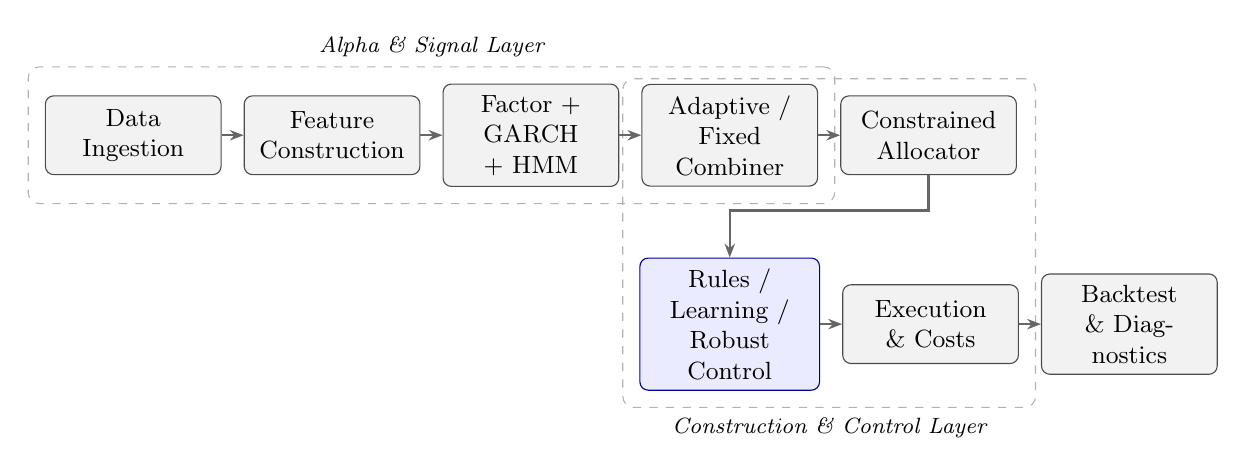
\begin{tikzpicture}[
  node distance = 0.45cm and 0.28cm,
  box/.style = {
    rectangle, rounded corners=3pt,
    draw=black!70, fill=gray!10,
    text width=1.95cm, align=center,
    font=\small, minimum height=1.0cm,
    inner sep=4pt
  },
  rlbox/.style = {
    rectangle, rounded corners=3pt,
    draw=blue!60!black, fill=blue!8,
    text width=2.0cm, align=center,
    font=\small, minimum height=1.0cm,
    inner sep=4pt
  },
  arr/.style = {-{Stealth[length=5pt]}, thick, black!60},
  groupbox/.style = {
    draw=black!30, dashed, rounded corners=4pt,
    fill=none, inner sep=6pt
  }
]
\node[box] (data)    {Data\\Ingestion};
\node[box, right=of data]    (feat)    {Feature\\Construction};
\node[box, right=of feat]    (alpha)   {Factor +\\GARCH + HMM};
\node[box, right=of alpha]   (comb)    {Adaptive /\\Fixed Combiner};
\node[box, right=of comb]    (alloc)   {Constrained\\Allocator};
\node[rlbox, below=0.9cm of comb] (control) {Rules / Learning /\\Robust Control};
\node[box, right=of control] (exec)    {Execution\\\& Costs};
\node[box, right=of exec]    (bt)      {Backtest\\\& Diagnostics};

\draw[arr] (data)  -- (feat);
\draw[arr] (feat)  -- (alpha);
\draw[arr] (alpha) -- (comb);
\draw[arr] (comb)  -- (alloc);
\draw[arr] (alloc.south) -- ++(0,-0.45) -| (control.north);
\draw[arr] (control) -- (exec);
\draw[arr] (exec) -- (bt);

\begin{scope}[on background layer]
  \node[groupbox, fit=(data)(feat)(alpha)(comb),
        label={[font=\footnotesize\itshape]above:Alpha \& Signal Layer}] {};
  \node[groupbox, fit=(alloc)(control)(exec),
        label={[font=\footnotesize\itshape]below:Construction \& Control Layer}] {};
\end{scope}
\end{tikzpicture}
\caption{High-level architecture of the revised quantitative trading pipeline.
The alpha layer is intentionally finance-first, the allocator builds a capped
and turnover-aware target book, and the control comparison focuses on how much
of that book to express rather than on a second stock-selection problem. The
fixed components are the data, alpha, and allocator stack; the compared
components are the control families that reshape how the target book is
expressed. Those compared families span simple rules, contextual bandits,
supervised control, robust optimization, predictive control, and RL.}
\label{fig:architecture}
\end{figure*}

\subsection{Software Structure}

Table~\ref{tab:modules} summarizes the package decomposition that supports the
frozen-bundle workflow. The separation is intentional: alpha construction,
control comparison, backtesting, and plotting are kept in distinct modules so
that the reported artifact bundle can be regenerated and audited component by
component.

\begin{table*}[t]
\centering
\caption{Module-level decomposition of the \texttt{quant\_stack} package.}
\label{tab:modules}
\small
\begin{tabular}{@{} l p{0.78\textwidth} @{}}
\toprule
\textbf{Module} & \textbf{Responsibility} \\
\midrule
\texttt{config.py}   & Universe definition, global constants, and external series identifiers \\
\texttt{data.py}     & Market price/volume ingestion, macro series (FRED / BLS fallback), and SEC company facts \\
\texttt{alpha.py}    & Cross-sectional factors, GARCH volatility, HMM regime, and adaptive or fixed signal combination \\
\texttt{rl.py}       & Portfolio controller, state construction, and end-to-end PPO benchmark interfaces \\
\texttt{pipeline.py} & Walk-forward backtest orchestration and online RL update loop \\
\texttt{evaluation.py} & Control-method comparison, ablation, rolling-window robustness, significance tests, and artifact export \\
\texttt{plots.py}    & Equity-curve, drawdown, controller-behavior, robustness, and reward-ablation figures \\
\texttt{main.py}     & CLI entry point and compatibility wrapper \\
\bottomrule
\end{tabular}
\end{table*}

\section{Data and Feature Construction}

\subsection{Universe}

The revised frozen-bundle uses two disjoint universes rather than a single
development basket. Universe A contains 77 traded tickers spread across
technology, financials, healthcare, consumer staples, energy, industrials,
materials, real estate, utilities, communications, consumer discretionary, and
diversifier exposures such as GLD, TLT, and VNQ. Universe B contains 75
non-overlapping names with stronger mid-cap technology, biotech, REIT,
midstream-energy, and materials tilts. SPY serves as the passive equity
benchmark in both universes so that the control comparisons remain externally
calibrated on the same calendar windows.

\subsection{Data Sources}

Daily prices and volumes are sourced via \texttt{yfinance}. When a
\texttt{FRED\_API\_KEY} is available, macro data are drawn directly from FRED;
in its absence, the system falls back to BLS and U.S.\ Treasury Fiscal Data.
SEC company facts are incorporated when \texttt{SEC\_USER\_AGENT} is set,
enabling a light fundamentals layer without requiring a proprietary data
subscription.

\subsection{Macro Regime Inputs}

When available, the macro sleeve includes the 10-year yield, 2-year yield,
federal funds rate, unemployment rate, and term spread. The updated research
design also incorporates stress-sensitive FRED series including the VIX, the
ICE BofA high-yield option-adjusted spread, and a dollar-index proxy. These
variables do not form a standalone alpha book. Instead, they help create a
macro regime belief that is blended with the HMM regime estimate and provide
additional context for risk-off states.

\subsection{Information-Timing Contract}

The pipeline makes its feature-availability assumptions explicit. Macro inputs are
shifted forward by a configurable number of trading days before they are allowed
into the backtest. This is still weaker than a true real-time vintage database,
because it does not model revisions, but it is materially stronger than using
the final macro history with no delay assumption at all.

Fundamental inputs are handled more conservatively. The SEC quality signal is
still a static cross-sectional research prior rather than a fully point-in-time
fundamentals panel. For that reason the research engine supports a strict timing
mode in which the SEC quality sleeve is disabled and macro inputs are forced to
use the largest configured lag. The point of this design is not to pretend that
point-in-time fundamentals are already solved, but rather to make the timing
caveat measurable and visible in the evaluation workflow.

\section{Methodology}

The methodology treats portfolio control as risk shaping rather than as a
second forecasting contest. The alpha engine and constrained allocator are held
fixed; what changes across methods is how each controller reshapes the induced
return distribution through exposure rules, robust selection, payoff
transformation, predictive planning, or learned mixtures.

\subsection{Problem Formulation}

Let $r_{t+1} \in \mathbb{R}^N$ denote next-period asset returns for a universe of
$N$ tradable assets. At time $t$, the system observes a feature state
$x_t \in \mathcal{X}$ constructed from cross-sectional factor values,
volatility forecasts, regime beliefs, macro inputs, recent portfolio returns,
and allocation summaries. The alpha layer maps these features into an
expected-return score vector $\alpha_t \in \mathbb{R}^N$ and a confidence
vector $c_t \in \mathbb{R}^N$.

The control layer then chooses a portfolio allocation $w_t$ and a cash
allocation. The one-step objective is not written as a pure return-maximization
problem. Instead, it is implicitly multi-objective: maximize long-run wealth
while limiting drawdown, volatility, and unnecessary turnover. This is the
reason the project separates alpha estimation from control: the two tasks
operate on different time scales and carry different inductive biases.
Importantly, the learned controller does not forecast $r_{t+1}$ directly; it
maps a state summarizing alpha opportunity, current allocation, and recent
portfolio outcomes into exposure and overlay decisions.

\subsection{Cross-Sectional Factor Model}

The factor sleeve combines four z-scored components: momentum, a value proxy, a
quality proxy, and a low-volatility tilt. Letting $m_i$, $v_i$, $q_i$, and
$\ell_i$ denote the standardized scores for asset $i$, the composite factor
score is
\[
f_i = 0.30 m_i + 0.25 v_i + 0.25 q_i + 0.20 \ell_i.
\]
This choice reflects a balanced, multi-style factor book rather than a single
directional bet. In this architecture, the factor book is the dominant alpha
source, with the other retained sleeves acting mainly as stabilizers or
confidence modifiers rather than as separate return engines.

\subsection{Volatility and Regime Models}

Each name receives a GARCH(1,1) forecast
\[
\sigma_t^2 = \omega + \alpha_1 \epsilon_{t-1}^2 + \beta_1 \sigma_{t-1}^2,
\]
where $\omega > 0$, $\alpha_1 \geq 0$, and $\beta_1 \geq 0$ are the intercept,
ARCH, and GARCH coefficients respectively. This conditional variance estimate
is used for confidence scaling and risk awareness. Separately, a two-state HMM
produces a bull-versus-bear regime belief. The final regime signal is
\[
\text{RegimeBelief}_t =
0.75 \cdot \text{HMMBelief}_t +
0.25 \cdot \text{MacroBelief}_t.
\]

\subsection{Adaptive Alpha Combination}

Let $s^{(k)}_{i,t}$ denote the signal from source $k$ for asset $i$ at time $t$.
The expected return score is formed as
\[
\alpha_{i,t} = \sum_k w^{(k)}_t s^{(k)}_{i,t},
\]
where the source weights $w^{(k)}_t$ adapt over time based on recent realized
signal quality. In the implementation, this is proxied by recent Spearman
information coefficients between source scores and realized returns.

This adaptive weighting is important because the retained sleeves are not
equally informative across all market states. In this architecture, however,
adaptive weighting is explicitly treated as an ablation rather than as an
article of faith. Fixed weights remain a strong baseline precisely because the
archived bundle suggests that adaptive combination does not obviously add value
in the current sample.

\subsection{Constrained Allocator}

The controller is not handed raw scores and asked to build a book from scratch.
Instead, the pipeline inserts a constrained intermediate allocator between the
alpha layer and the control layer. The factor-anchored target book is
\[
w_t^{\text{target}} =
0.90\,w_t^{\text{factor}} +
0.10\,w_t^{\text{stabilizer}},
\]
where the stabilizer is a long-only minimum-variance-style portfolio estimated
from a Ledoit--Wolf shrinkage covariance matrix.

The allocator solves a small regularized problem of the form
\[
\begin{aligned}
\min_w \quad &
\lambda_{\mathrm{risk}} w^\top \Sigma_t w
- \lambda_{\alpha}\alpha_t^\top w \\
&+ \lambda_{\mathrm{anchor}}\lVert w - w_t^{\mathrm{target}} \rVert_2^2 \\
&+ \lambda_{\mathrm{turn}}\lVert w - w_{t-1} \rVert_2^2
\end{aligned}
\]
subject to $w_i \ge 0$, $\sum_i w_i = 1$, per-asset caps, and group
concentration limits. This intermediate layer is not only an architectural
convenience; it reflects the practical fact that many real portfolio systems
mediate between forecast signals and final positions through a constrained
allocator.

\subsection{Control Methods}

The completed frozen-bundle compares six families of control methods built on
the same finance-first alpha engine and constrained allocator.
\begin{enumerate}[leftmargin=1.5em, itemsep=2pt, topsep=4pt]
\item \textbf{Alpha and fixed-rule baselines.} The suite includes
      \texttt{factor\_only}, a fixed 95\% allocator, volatility targeting,
      drawdown-based deleveraging, regime-aware rules, and simple rule
      ensembles.
\item \textbf{Contextual bandits.} Three lightweight bandit controllers are
      evaluated: LinUCB, Thompson sampling, and an $\varepsilon$-greedy linear
      controller.
\item \textbf{Supervised control.} An expanding-window classifier predicts the
      most attractive exposure bucket from the same compact state summary.
\item \textbf{Robust optimization.} A CVaR-aware robust allocator augments the
      constrained optimizer with downside-sensitive risk control and is the
      main non-learning advanced comparator.
\item \textbf{Predictive control.} A model-predictive controller (MPC)
      performs receding-horizon exposure planning with explicit turnover,
      stress, and stabilizer penalties, providing a structured control-theory
      comparator.
\item \textbf{RL comparators.} Tabular portfolio Q-learning remains as a direct
      learned-controller baseline, and end-to-end PPO is retained as a
      monolithic comparator outside the main control-comparison suite.
\end{enumerate}

\subsection{Control as Risk-Shaping Optimization}

The revised paper interprets portfolio control as a risk-shaping problem rather
than as a pure forecasting problem. Let $R^\pi$ denote the realized return
distribution induced by controller $\pi$ on top of the fixed alpha engine and
constrained allocator. Then the generic objective is
\[
\begin{aligned}
\max_{\pi}\;& \mathbb{E}[R^\pi] \\
\text{s.t.}\;& \mathcal{L}(R^\pi)\ \text{is shaped toward acceptable downside behavior,}
\end{aligned}
\]
or, equivalently, $\max_{\pi}\ \mathbb{E}[R^\pi]-\lambda\mathcal{L}(R^\pi)$ for
an implicit risk functional $\mathcal{L}$. In that sense, all controllers can
be viewed as different approximations to risk-shaping operators applied to the
return distribution.

More formally, let $F_t^{(0)}$ denote the reference one-step return
distribution generated by the fixed alpha engine and constrained allocator
before a controller intervenes. Each controller then induces an operator
$\mathcal{S}_\pi$ such that
\[
\begin{aligned}
F_t^\pi
&= \mathcal{S}_\pi\!\left(F_t^{(0)}\right) \\
&= \left(\mathcal{T}_\pi \circ \mathcal{Q}_\pi\right)\!\left(F_t^{(0)}\right).
\end{aligned}
\]
Here $\mathcal{Q}_\pi$ is a \emph{selection operator} that changes portfolio
weights, scenario weights, or exposure levels, and $\mathcal{T}_\pi$ is an
\emph{outcome operator} that reshapes realized payoffs after a portfolio has
been selected. The controller search problem is therefore
\[
\begin{aligned}
\pi^\star
= \arg\max_{\pi \in \Pi}\;& \mathbb{E}_{F_t^\pi}[R] \\
&- \lambda \mathcal{L}(F_t^\pi).
\end{aligned}
\]
This is the paper's central theoretical lens. Rules, bandits, RL, CMDP, CVaR,
convexity, and council meta-control differ not mainly in prediction, but in the
class of risk-shaping operators they apply to the same underlying return
distribution. Rules, bandits, RL, and CMDP mainly approximate selection
operators $\mathcal{Q}_\pi$; convexity is primarily an outcome operator
$\mathcal{T}_\pi$; the council learns a mixture operator over expert policies;
and the winning controller can be written compactly as
$\mathcal{S}_{D+}=\mathcal{T}_{\text{convex}}\circ\mathcal{Q}_{\text{CVaR}}$.

This operator lens also connects the controller comparison to classical distortion-risk ideas. Dual-theory and distorted-expectation views interpret risk control as transforming probabilities or outcomes rather than only changing point forecasts \cite{yaari1987,schmeidler1989,wang2000}. In that language, CVaR is a coherent left-tail distortion applied during portfolio selection, while the convexity layer is a discrete outcome distortion applied to realized returns. The framework therefore does more than label winners: it classifies controllers by how they reshape the induced return distribution.

The key empirical result is therefore not only that the robust family wins, but
that its strongest variants compose two different risk-shaping operations. Most
learning-based controllers in the bundle mainly act through a selection
operator $\mathcal{Q}_\pi$. The convexity layer contributes through an outcome
operator $\mathcal{T}_\pi$. The peak Universe-A controller is the first one in
the study that combines both in a structured way.

\begin{center}
\small
\begin{tabular}{@{} p{0.26\linewidth} p{0.62\linewidth} @{}}
\toprule
\textbf{Method family} & \textbf{Risk-shaping interpretation} \\
\midrule
Rules & Heuristic constraints on exposure and participation \\
Bandits & Contextual reward maximization under noisy feedback \\
RL & Sequential policy optimization over coarse actions \\
CMDP & Constrained policy optimization with a dual penalty \\
CVaR & Coherent left-tail risk minimization in portfolio selection \\
Convexity & Payoff transformation in stressed states \\
Meta-control & Mixture of policies with adaptive expert weights \\
\bottomrule
\end{tabular}
\end{center}

\subsection{Theoretical Grounding}

\paragraph{Proposition 1 (tail-shaping improvement under mild regularity).}
Let $R$ be a one-step portfolio return with continuous distribution supported on
$[r_{\min}, r_{\max}]$, let $q_\alpha:=q_\alpha(R)<\tau$ denote the lower
$\alpha$-quantile, and define
\[
g_m(r)=r-c(m)+\lambda_m(\tau-r)_+^2.
\]
Assume (i) $g_m$ is nondecreasing on $[r_{\min},\tau]$, equivalently
$2\lambda_m(\tau-r_{\min})\le 1$, and (ii)
$c(m)\le \lambda_m(\tau-q_\alpha)^2$. Then
\begin{align*}
\mathbb{E}[g_m(R)]
&=\mathbb{E}[R]-c(m)+\lambda_m \mathbb{E}\!\left[(\tau-R)_+^2\right], \\
\operatorname{CVaR}_\alpha(-g_m(R))
&\le \operatorname{CVaR}_\alpha(-R)-\delta_\alpha(m),
\end{align*}
where $\delta_\alpha(m):=\lambda_m(\tau-q_\alpha)^2-c(m)\ge 0$.

\emph{Proof.} Let $A_\alpha:=\{R\le q_\alpha\}$. Because $q_\alpha<\tau$, for
every $r\in A_\alpha$,
\[
g_m(r)-r \ge -c(m)+\lambda_m(\tau-q_\alpha)^2 = \delta_\alpha(m).
\]
Assumption (i) preserves the ordering of tail states on $[r_{\min},\tau]$, so
the worst $\alpha$-tail of $g_m(R)$ is still attained on $A_\alpha$. Therefore
\begin{align*}
\operatorname{CVaR}_\alpha(-g_m(R))
&= -\mathbb{E}[g_m(R)\mid A_\alpha] \\
&\le -\mathbb{E}[R\mid A_\alpha]-\delta_\alpha(m) \\
&= \operatorname{CVaR}_\alpha(-R)-\delta_\alpha(m).
\end{align*}
The expectation identity follows by expanding $g_m(R)$ pointwise and taking
expectations. Thus convexity reduces lower-tail risk whenever the protected-tail
gain dominates carry. \hfill $\square$

In the reference D+ split, $\tau=0$, the strong-mode coefficient is
$\lambda_m=4$, and the observed raw-return minimum is about $-11.3\%$, so
assumption (i) implies $2\lambda_m(\tau-r_{\min})\approx 0.90<1$ and is
satisfied in the reported sample. The key implication is operational rather
than cosmetic: performance improvements arise not from better prediction, but
from improved shaping of the return distribution's left tail.

\subsection{CVaR-Robust Controller}

Method D replaces scalar exposure scaling with a direct long-only weight
optimizer built on the same constrained target book. Let $\mu_t$ denote the
combined alpha scores scaled into daily-return units and let $\Sigma_t$ denote
the Ledoit--Wolf covariance estimate. The controller solves
\begin{align*}
\min_w \quad &
\lambda_{\mathrm{risk}} w^\top \Sigma_t w
- \lambda_{\alpha}\mu_t^\top w
+ \lambda_{\mathrm{anchor}}\lVert w-w_t^{\mathrm{target}} \rVert_2^2
\\
&+ \lambda_{\mathrm{turn}}\lVert w-w_{t-1} \rVert_2^2
+ \lambda_{\mathrm{CVaR}} \operatorname{CVaR}_{0.95}(L_t(w)),
\end{align*}
subject to the same long-only, sum-to-one, position-cap, and concentration
constraints as the allocator. The loss term $L_t(w)$ is estimated from 500
Gaussian return scenarios whose mean is given by the current alpha scores and
whose covariance is given by the shrinkage estimator. In implementation,
$\lambda_{\mathrm{CVaR}}$ is increased when regime belief deteriorates and when
recent drawdown exceeds 5\%, so the robust controller becomes more conservative
in stressed states without changing the underlying alpha engine.

\subsection{Convexity-Aware Protection Modes}

The D+ extension does not replace the robust optimizer. It post-processes the
net portfolio return produced by the controller through a small three-mode
payoff-shaping layer:
\[
\tilde r_t = r_t^{\mathrm{net}} - c(m_t)
+ \lambda_{m_t}\max(0,\tau-r_t^{\mathrm{net}})^2,
\]
where $m_t \in \{0,1,2\}$ corresponds to none, mild, or strong protection and
$\tau=0$ in the archived bundle. The daily carry schedule is $(0,1.5,4.0)$ bp
and the quadratic coefficients are $(0,1.5,4.0)$. Strong protection activates
whenever recent drawdown is at most $-10\%$, realized annualized volatility is
at least 26\%, or regime belief falls below 0.30. Mild protection activates
whenever drawdown is at most $-5\%$, volatility is at least 18\%, or regime
belief falls below 0.45. Otherwise the mode is off. The layer therefore pays
small carry in stressed states and only produces benefit on left-tail days,
making D+ a stylized convex protection overlay rather than a separate options
engine. The archived diagnostics record convexity mode frequencies, carry paid,
and benefit realized by regime.

\subsection{Logistic and MLP Meta-Control}

Controller E is a soft council over three meaningful experts: A4 regime rules,
B1 LinUCB, and D CVaR-robust. Each expert produces a candidate book
$b_t^{(k)}$, and the council outputs
\[
b_t = \sum_{k=1}^3 \pi_k(x_t)b_t^{(k)}.
\]
The gate state is intentionally small: alpha strength, recent drawdown,
realized volatility, and regime belief.
The gate is a multinomial logistic model retrained every 63 trading days once
at least 40 labeled examples are available. Before retraining is possible, it
starts from a 20/20/60 prior over regime rules, LinUCB, and CVaR-robust and
tilts that prior toward CVaR under risk pressure and toward LinUCB when alpha
strength is high. Labels are generated ex post from same-day expert net
returns: the best realized expert becomes the target class for the next gate
update. This keeps the council interpretable and lightweight: it is a
supervised meta-controller over structured experts rather than a black-box RL
policy over the full portfolio. E+ applies the same convexity layer after the
blended council book is formed.

Candidate G keeps the same expert set and mixing equation but replaces the
logistic gate with a small multilayer perceptron. Its gate state is a
16-dimensional environment feature vector built from trailing alpha quality,
risk and volatility, market stress, regime, trend, and concentration
statistics. The default hidden-layer layout is $(32,16)$ with early stopping
and $\ell_2$ regularization. The MLP is retrained every 63 trading days once
at least 60 labeled examples are available; before that point it falls back to
the same heuristic prior used by the council. G+ applies the same convexity
layer after the blended MLP-controlled book is formed. This pair isolates
whether a more expressive gate improves on the lighter logistic council
without changing the underlying experts.

\subsection{CMDP-Lagrangian Control}

Candidate F keeps the same compact discrete control problem as tabular
Q-learning, but it modifies the learning objective to a constrained MDP. Its
state uses the same discretized summary of alpha strength, recent drawdown,
realized volatility, and regime belief, and the action ladder is the
invested-fraction set $\{0.82, 0.90, 0.95, 0.98, 1.00\}$. The default
constrained problem is
\[
\max_{\pi}\; \mathbb{E}[R_t]
\quad \text{s.t.} \quad
\mathbb{E}[C_t] \le \kappa,
\]
where $C_t$ is a drawdown cost and $\kappa=0.12$ in the archived bundle. The
implementation uses a Lagrangian relaxation,
\begin{align*}
\tilde R_t &= R_t - \lambda_t(C_t-\kappa), \\
\lambda_{t+1} &= \max(0,\lambda_t + \eta(C_t-\kappa)),
\end{align*}
with $\lambda_0=1.0$ and $\eta=0.05$. By default
$C_t = \max(0,-\mathrm{DD}_{t+1})$, i.e.\ the positive part of next-step recent
drawdown; an alternative tail-loss version replaces this with
$\max(0,-r_t-\delta)$ using $\delta=1\%$. The CMDP candidate therefore tests
whether constrained learning can close the gap to robust optimization without
changing state size or model capacity.

\subsection{Portfolio RL}

The portfolio RL state is deliberately minimal. It is constructed from the
current alpha-score cross-section, the current portfolio-weight summary, and
recent portfolio returns.

If the RL agent chooses invested fraction $b_t$ and active overlay size $\tau_t$,
the final invested portfolio is approximately
\[
w_t =
b_t \left[(1-\tau_t)w_t^{\text{target}} + \tau_t w_t^{\text{satellite}}\right].
\]
The satellite sleeve is not a fully independent book; it tilts the factor target
toward the strongest alpha names. This keeps the full pipeline close to the
working factor engine while still letting RL modulate aggressiveness.

\subsection{Reward Design}

The default reward is a Sortino-style objective. In compact form,
\[
R_t^{\mathrm{portfolio}}
= \frac{r_t - \hat{\mu}_t}{\hat{\sigma}^{\mathrm{down}}_t + \varepsilon},
\]
where $\hat{\mu}_t$ is a running mean and
$\hat{\sigma}^{\mathrm{down}}_t$ is a running downside-deviation estimate. The
agent is therefore rewarded for improving return relative to downside risk
rather than for taking more total variance in absolute terms.

The research runner also supports reward-function ablations over
differential-Sharpe, raw-return, Sortino, and mean-variance formulations. This
matters because reward design is one of the least observable but most important
degrees of freedom in RL-for-finance systems. Because reward specification
changes the controller's operating point, it should be treated as a
methodological degree of freedom rather than as a neutral implementation detail.

\subsection{No-Trade Band and Transaction Costs}

To reduce turnover drag, a rebalance band suppresses small changes in target
weights. When only part of the portfolio is changed, the active weights are
rescaled to preserve the desired capital budget.

The backtest includes a three-part execution-cost approximation. For each
rebalance, the strategy pays a fixed basis-point fee on turnover, an additional
penalty proportional to turnover times realized volatility, and a size penalty
linked to the largest one-name weight change. In symbols,
\[
\mathrm{TC}_t
= c_0 \cdot \mathrm{turnover}_t
+ c_1 \cdot \mathrm{turnover}_t \cdot \hat{\sigma}_t
+ c_2 \cdot \max_i |\Delta w_{i,t}|.
\]
This is not a full execution simulator, but it pushes the daily allocator away
from unrealistic churn and makes the rebalance band economically meaningful
rather than purely cosmetic.

\section{Experimental Design}

The evaluation protocol uses two disjoint universe runs, each with 3{,}269
daily observations from April 2, 2013 through March 30, 2026. Each archived
bundle contains the same core suite: legacy ablations, 19 control-method
candidates across three train/test split settings, a strict-timing check, six
rolling windows, four cost settings, three rebalance-band settings, three
macro-lag settings, four reward settings, and five blocked time-series CV
folds. Reported claims are tied to the archived CSV and figure artifacts
released with the codebase, manuscript, and bundle layout in the public
repository \url{https://github.com/ioan-hedea/quant-paper-lab}. Exact bundle
paths are listed in the appendix.

Within that archived suite, action ladders, optimizer settings, reward choices,
and comparison baselines are held fixed across ablations, split-fraction tests,
rolling-window robustness slices, and significance calculations. The control
comparison itself uses train fractions \{0.4, 0.5, 0.6\} for nearly all methods
and replaces the middle split with a 0.75/0.25 schedule for the Q-learning
comparator to give the tabular learner a more favorable sample budget. The
evaluated family now includes no-control exposure, simple rules, ensembles,
contextual bandits, supervised control, CVaR-aware robust optimization,
convexity-aware protection, council meta-control, MLP meta-control,
CMDP-Lagrangian control, and RL under the same cost and timing discipline.

At each date, the revised pipeline executes the following sequence. First,
factor, GARCH, HMM, macro, and optional SEC features are generated from the
available data. These are combined into expected-return scores via either the
adaptive or fixed combiner. The constrained allocator produces the target book.
The chosen controller then decides how much of that book to express via
invested fraction and active overlay size. For the robust and council
extensions, an optional convexity mode can then apply a stylized carry cost and
left-tail payoff shaping term before the final realized portfolio return is
recorded. That realized return is finally used to update the value table or
policy state when the controller is learned.

\subsection{Benchmark Logic}

The benchmark set is chosen to isolate different sources of value. SPY measures
whether the pipeline adds value relative to standard passive equity exposure.
The factor-only benchmark isolates the pure alpha layer without any controller
overlay. Because the archived bundle already uses a broad 77-ticker universe,
this factor benchmark is also informative about what the diversified opportunity
set can do without learned control. Comparing the full pipeline against the
factor-only benchmark is particularly important because it reveals whether
learning is adding value as a controller or merely acting as a drag on a strong
signal engine.

The newer comparison baselines sharpen that logic further. The volatility
targeting baseline asks whether most of the observed improvement can be matched
by simple inverse-vol scaling. The drawdown-based deleveraging baseline asks
whether a threshold rule can replicate the control layer's protection effect.
The end-to-end PPO baseline addresses the paper's most distinctive
architectural question: if one hands the same state information to a monolithic
policy, does it outperform a hybrid design in which finance-specific modules
produce the target book and RL only controls how aggressively to express it?
These baselines are deliberately strong because they represent the kinds of
simple overlays a practitioner would try before accepting the complexity of RL.

\section{Evaluation Metrics}

The reporting suite includes annualized return, annualized volatility, Sharpe
ratio, Sortino ratio, maximum drawdown, Calmar ratio, and return-distribution
diagnostics including a daily 5\% Value-at-Risk estimate.

If $\{r_t\}_{t=1}^T$ denotes daily portfolio returns and $r_f$ is the annual
risk-free rate, then the annualized Sharpe ratio is
\[
\text{Sharpe} = \frac{252 \, \bar{r} - r_f}{\sqrt{252}\,\hat{\sigma}(r) + \varepsilon}.
\]
The Sortino ratio replaces total volatility with downside volatility, while the
Calmar ratio scales annualized return by the magnitude of maximum drawdown. Each
metric emphasizes a different aspect of the return distribution, which matters
in this project because the controller is explicitly designed to reshape risk,
not merely to maximize mean return. Table~\ref{tab:metrics} focuses on the
primary comparison metrics used in the main strategy table: return, volatility,
Sharpe, maximum drawdown, and Calmar. Sortino and Value-at-Risk are retained as
secondary diagnostics in the text, reward-ablation evidence, and archived
research artifacts.

\section{Results}

Three answers organize the results. First, the robust family defines the
frontier in both universes, with \texttt{D\_plus\_convexity} strongest in
Universe A and plain \texttt{D\_cvar\_robust} the more portable winner in
Universe B. Second, simple rules remain credible downside-control baselines but
do not displace the robust frontier. Third, learning helps most when used as
meta-control over structured experts; learning-first controllers do not
dominate the shared alpha engine.

\begin{table}[t]
\centering
\footnotesize
\caption{Scannable summary of the main controller families.}
\label{tab:family_summary}
\begin{tabular}{@{} p{1.35cm} p{1.15cm} p{1.65cm} p{1.45cm} @{}}
\toprule
\textbf{Family} & \textbf{Role} & \textbf{Strength} & \textbf{Weakness} \\
\midrule
Robust & Risk control & Best Sharpe frontier in this evaluation & Can be conservative \\
Convexity & Tail shaping & Strong conditional edge in Universe A & Less portable across universes \\
Meta-control & Adaptive mixing & Best learned region of the design space & Still below robust frontier \\
MPC & Predictive control & Strong low-drawdown profile & Lower upside capture \\
\bottomrule
\end{tabular}
\end{table}

\paragraph{Key findings.}
\begin{itemize}[leftmargin=1.2em, itemsep=2pt, topsep=3pt]
\item In this frozen-bundle evaluation, the robust family defines the frontier.
\item Convexity adds a conditional edge when left-tail asymmetry is strong.
\item Learning is most useful as meta-control over already-credible experts.
\end{itemize}

\subsection{Main Result: Control Comparison}

The main result is the completed 19-method control-comparison suite.
Table~\ref{tab:metrics} reports mean annualized performance across the three
train/test split settings used in the frozen-bundle.

\begin{table*}[t]
\centering
\small
\caption{Representative controller summary across the two disjoint universes.
All methods share the same finance-first alpha engine and constrained allocator.
Universe A is the original 77-ticker bundle; Universe B is the zero-overlap
75-ticker bundle. Full 19-method rankings remain in the archived CSVs.
Annualized figures.}
\label{tab:metrics}
\begin{tabular}{@{} l r r r r r r @{}}
\toprule
\textbf{Controller} & \textbf{A Ret.} & \textbf{A Sh.} & \textbf{A Max DD} & \textbf{B Ret.} & \textbf{B Sh.} & \textbf{B Max DD} \\
\midrule
No control (alpha engine) & 9.3\% & 0.41 & $-$19.5\% & 10.5\% & 0.58 & $-$12.0\% \\
\midrule
A1: Fixed & 9.0\% & 0.40 & $-$18.6\% & 10.1\% & 0.58 & $-$11.3\% \\
A4: Regime rules & 8.8\% & 0.42 & $-$15.8\% & 9.4\% & 0.55 & $-$10.4\% \\
\midrule
B1: LinUCB & 8.8\% & 0.42 & $-$17.5\% & 9.9\% & 0.58 & $-$10.8\% \\
\midrule
C: Supervised & 8.7\% & 0.40 & $-$19.0\% & 9.8\% & 0.59 & $-$11.7\% \\
\midrule
D: CVaR-robust & 17.7\% & 0.81 & $-$26.4\% & \textbf{14.0\%} & \textbf{0.70} & $-$14.5\% \\
\textbf{D+: CVaR + convexity} & \textbf{17.8\%} & \textbf{0.84} & \textbf{$-$18.6\%} & 12.9\% & 0.64 & $-$14.1\% \\
\midrule
E: Council & 12.8\% & 0.65 & $-$20.9\% & 11.6\% & 0.65 & $-$12.4\% \\
G: MLP meta & 12.2\% & 0.61 & $-$19.8\% & 11.2\% & 0.61 & $-$12.3\% \\
\midrule
F: CMDP-Lagrangian & 8.2\% & 0.37 & $-$18.5\% & 9.4\% & 0.54 & $-$11.0\% \\
H: MPC & 6.0\% & 0.56 & $-$6.7\% & 6.1\% & 0.64 & \textbf{$-$3.9\%} \\
RL: Q-learning & 8.3\% & 0.43 & $-$15.0\% & 9.9\% & 0.58 & $-$10.9\% \\
\bottomrule
\end{tabular}
\end{table*}

\paragraph{Comparison to Passive Benchmark (SPY).}
As an external calibration point, SPY averages 14.0\% annualized return,
18.8\% volatility, 0.56 Sharpe, and $-$30.6\% maximum drawdown across the same
three split windows in both universes. It is not shown as a row in
Table~\ref{tab:metrics} because SPY is a passive benchmark rather than a
controller applied to the shared alpha engine. In Universe A, only the robust
pair \texttt{D} and \texttt{D+} clearly exceed SPY on both mean return and mean
Sharpe. In Universe B, plain \texttt{D} roughly matches SPY on mean return
while exceeding it on Sharpe and drawdown, whereas the council and MPC variants
exceed SPY on Sharpe and drawdown but not on mean return.

Among the learned methods, \texttt{E\_council} is now the closest learned SPY
challenger overall. In Universe B it reaches 11.6\% mean return, 0.65 Sharpe,
and $-$12.4\% mean maximum drawdown, so it trails SPY on upside but materially
improves the downside profile. The MLP gate remains competitive, but it does
not improve on the simpler council in either universe.

\begin{table}[t]
\centering
\small
\caption{Robust winner versus SPY in each universe across the same three
control-comparison splits.}
\label{tab:robust_spy}
\resizebox{\columnwidth}{!}{%
\begin{tabular}{@{} l l r r r @{}}
\toprule
\textbf{Universe} & \textbf{Winner} & \textbf{Return} & \textbf{Sharpe} & \textbf{Max DD} \\
\midrule
A benchmark & D+: CVaR + convexity & 17.8\% vs 14.0\% & 0.84 vs 0.56 & $-$18.6\% vs $-$30.6\% \\
B benchmark & D: CVaR-robust & 14.0\% vs 14.0\% & 0.70 vs 0.56 & $-$14.5\% vs $-$30.6\% \\
\bottomrule
\end{tabular}}
\end{table}

Table~\ref{tab:robust_spy} makes the passive comparison explicit. In Universe A,
\texttt{D+} achieves higher return and Sharpe than SPY while also reducing
drawdown. In Universe B, plain \texttt{D} is the strongest direct challenger:
it roughly matches SPY on return, improves Sharpe, and cuts drawdown by more
than half. The correct claim is not that the paper ``beats SPY'' in general,
but that the robust family provides the strongest point-estimate SPY challenger
under the shared control-comparison protocol. This SPY comparison is economic
calibration rather than the paper's scientific contribution: the contribution
is a principled comparison of control mechanisms under shared alpha, timing,
and cost assumptions.

The main answer to \textbf{RQ1} is now explicitly cross-universe. The robust
family remains strongest in both universes, but the best robust variant is not
universal. In Universe A, \texttt{D\_plus\_convexity} is the clear winner at
0.84 mean Sharpe and 0.95 Calmar, improving markedly on plain \texttt{D}. In
Universe B, plain \texttt{D\_cvar\_robust} is the strongest point estimate at
0.70 mean Sharpe, while \texttt{E\_council} and \texttt{H\_mpc} cluster just
below it near 0.65. The best single run in the entire comparison remains
\texttt{D\_plus\_convexity\_tf0.50} in Universe A, which reaches 21.4\%
annualized return with 1.00 Sharpe.

The main answer to \textbf{RQ2} is also positive. Simple rules can provide
competitive risk control, but the best simple rule is universe-dependent. In
Universe A, regime-aware rules reach 0.42 mean Sharpe with $-$15.8\% drawdown,
improving on the no-control alpha engine's 0.41 Sharpe and $-$19.5\% drawdown.
In Universe B, fixed exposure slightly edges regime rules on Sharpe
(0.58 versus 0.55) while keeping drawdown close to $-$11\%. No single method
dominates every risk metric: if shallow pathwise drawdown is the binding
constraint, the simple-rule and MPC families remain more attractive than the
highest-return robust controllers.

The main answer to \textbf{RQ3} is negative for the learning-based methods.
The learning stack does improve once it is reframed as meta-control rather than
standalone RL, but the strongest learned method is now the simpler
\texttt{E\_council}, not the more expressive MLP gate. The council reaches
about 0.65 Sharpe in both universes, with the MLP gate close behind at roughly
0.61. Both comfortably exceed the bandits, supervised controller,
CMDP-Lagrangian controller, and Q-learning RL in Universe A, while Universe B
is more forgiving and lifts almost every learned controller. Even so, the
learning-based methods still trail the robust frontier. Adding convexity to the
meta-controllers reduces drawdown modestly but gives back Sharpe, so the
evidence favors learned gating over learned payoff shaping. LinUCB remains the
best non-meta learner, CMDP-Lagrangian improves materially in Universe B, and
tabular Q-learning becomes respectable in Universe B without becoming a frontier
method.

Read as best-in-class representatives, the finished comparison is internally
coherent. Universe A's best simple rule is A4, while Universe B's is A1. B1 is
the best bandit in both universes. E is the best learned controller overall, G
is the strongest expressive learned gate but not an improvement over E, F is
the best constrained learner, H is the predictive-control and low-drawdown
frontier point, D is the most portable robust baseline, and D+ is the peak
performer when tail asymmetry is strongest. Table~\ref{tab:metrics} carries
the main cross-universe comparison in the body, while the full plot gallery for
both universes is collected in Appendix Figures~\ref{fig:control_overview}--
\ref{fig:mpcdiag}.

The MLP result is therefore still valuable, but it becomes a boundary result in
a different sense than before. A more expressive learned gate no longer
improves on the simpler council; it merely stays close to it. That confirms
that learning helps most at the meta-control layer, but also that the major
performance jump comes from moving from learned control to explicit robust risk
shaping, not from increasing gate complexity.

One important qualification is statistical rather than economic. The archived
controller-to-controller bootstrap tables now need to be read by universe. In
Universe A, the reference-split tests support \texttt{D+} against the main
learned and control-theory challengers. In Universe B, plain \texttt{D} is the
point-estimate winner, but the leading methods are tightly clustered and the
reference-split bootstrap does not show clean Sharpe separation among
\texttt{D}, \texttt{D+}, \texttt{E}, and \texttt{H}. Table~\ref{tab:robust_significance}
reports the key universe-specific comparisons, and Appendix
Table~\ref{tab:dplus_significance_full} reports the complete reference-split
pairwise table released with each bundle.

\begin{table}[t]
\centering
\small
\caption{Reference-split Sharpe deltas for the universe-specific robust winner
against key challengers under the cached block-bootstrap evaluation.}
\label{tab:robust_significance}
\resizebox{\columnwidth}{!}{%
\begin{tabular}{@{} l l r r r @{}}
\toprule
\textbf{Universe} & \textbf{Comparison} & \textbf{$\Delta$Sharpe} & \textbf{95\% CI} & \textbf{$p$-value} \\
\midrule
A & D+ -- E: Council & +0.26 & [0.02, 0.51] & 0.025 \\
A & D+ -- G: MLP meta & +0.33 & [0.01, 0.62] & 0.050 \\
A & D+ -- H: MPC & +0.44 & [0.08, 0.75] & 0.015 \\
A & D+ -- D: CVaR-robust & +0.10 & [$-$0.11, 0.32] & 0.705 \\
B & D -- D+: CVaR + convexity & +0.07 & [$-$0.01, 0.15] & 0.080 \\
B & D -- E: Council & +0.05 & [$-$0.16, 0.26] & 0.675 \\
B & D -- H: MPC & $-$0.02 & [$-$0.40, 0.40] & 0.950 \\
B & D -- SPY & +0.05 & [$-$0.58, 0.60] & 0.980 \\
\bottomrule
\end{tabular}}
\end{table}

Table~\ref{tab:robust_significance} makes the current statistical picture more
precise. In Universe A, the convexity-enhanced robust controller is not only
the point-estimate leader, but is also statistically superior to the council,
the MLP gate, and MPC on Sharpe at the reference split. Its edge over plain
\texttt{D} remains economically positive but not statistically decisive. In
Universe B, the point-estimate winner is plain \texttt{D}, yet the reference
split is much tighter: differences versus \texttt{D+}, the council, MPC, and
SPY are not statistically decisive on Sharpe. This Universe-A versus
Universe-B distinction is one of the paper's central findings: robust risk
shaping dominates both universes, but the extra convexity layer is strongly
supported only where left-tail asymmetry is pronounced.

The strongest practical insight from the new extensions is now conditional.
Convexity-aware payoff shaping directly addresses the earlier CVaR caveat in
Universe A: plain CVaR-robust has the deepest mean drawdown at $-$26.4\%, and
\texttt{D+} cuts that to $-$18.6\% while improving both Sharpe and Calmar. In
Universe B, the same convexity layer is milder in its effect: \texttt{D+}
reduces drawdown only slightly relative to plain \texttt{D} and gives back some
Sharpe, so the decisive winner becomes plain robust optimization rather than
the transformed version. The remaining Pareto tension is therefore between the
return-seeking robust stack in Universe A, the more portable plain-CVaR stack
in Universe B, and the clean defensive profile of \texttt{H\_mpc}.

\begin{quote}\small\noindent\textbf{RQ summary.} \textbf{RQ1:} In this frozen-bundle evaluation, the robust family is strongest in both universes, with \texttt{D+} best in Universe A and plain \texttt{D} best in Universe B. \textbf{RQ2:} Simple rules remain competitive for downside control, especially A4 in Universe A and A1 in Universe B. \textbf{RQ3:} Learning helps mainly as meta-control; no learning-first controller beats the robust frontier in this evaluation.\end{quote}

\paragraph{Regime-conditioned performance.}
Reference-split regime slices clarify why the universe ranking changes. In
Universe A, both \texttt{D} and \texttt{D+} remain essentially fully invested
through bull, neutral, and bear regimes at the reference split, but the
convexity mode intensifies sharply from 0.57 in bull states to 1.79 in bear
states. Average convexity carry rises from about 1 bp/day in bulls to 3.5
bp/day in bears, while average convexity benefit rises from roughly 0.5 bp/day
to 8.9 bp/day. That is exactly the setting in which \texttt{D+} improves on
plain \texttt{D}: the controller stays participatory while the left-tail
overlay becomes materially valuable.

Universe B is different. Plain \texttt{D} and \texttt{D+} again stay fully
invested, but the bear-state convexity benefit at the reference split is only
about 2.4 bp/day while the bear-state return remains slightly worse for
\texttt{D+} than for plain \texttt{D}. By contrast, \texttt{H\_mpc} sits near
35--36\% invested in all three regimes and limits the bear-state annualized
loss to about $-$6.7\% at 4.3\% volatility. The council remains highly invested
in both universes but keeps roughly 52--56\% weight on the CVaR expert and
shifts the residual weight between regime rules and LinUCB. These slices
explain why no single method dominates every environment: \texttt{D+} is the
best return-seeking robust controller when tail asymmetry is strong,
\texttt{D} is the more portable robust baseline, and \texttt{H\_mpc} is the
cleanest defensive controller when shallow drawdown is the binding objective.

\noindent\textit{Implication for the revised RQs.} \textbf{RQ1}: answered in
favor of the convexity-enhanced robust stack, with plain CVaR-robust as the
strongest non-extension baseline. \textbf{RQ2}: answered positively, with
regime-aware rules providing the strongest simple-rule baseline and vol-target
providing the shallowest drawdowns. \textbf{RQ3}: answered negatively for
learning-based control; even the learned meta-controllers remain below the best
optimization-based method.

\paragraph{Legacy pruning reference.}
A separate RL-centric pruning harness is retained for transparency, but its
role in the paper is diagnostic rather than central. Across both universes, the
factor core remains stronger than the legacy full learned stack, so the old
branch mainly marks the boundary of the design space and helps justify the
broader controller-comparison protocol. Detailed ablation, significance,
rolling-window, and reward diagnostics for that legacy branch are collected in
Appendix Section~\ref{sec:legacy_appendix}.


\section{Discussion}

The discussion focuses on mechanism rather than restating the leaderboard. The
main claim is that portfolio control is best understood here as risk shaping:
the strongest controllers improve the left tail of the induced return
distribution under shared alpha, timing, and cost assumptions. Across the two
universes, the same family dominates but not with a universal variant:
\texttt{D+} is strongest when tail asymmetry is pronounced, plain
\texttt{D} is the more portable robust baseline, and \texttt{H\_mpc} is the
clearest low-drawdown alternative.

The learning results sharpen that claim rather than weaken it. LinUCB is the
strongest non-meta learner, the council and MLP gates materially improve over
the standalone learners, and CMDP plus tabular RL do not close the gap to the
robust frontier in this evaluation. Learning therefore contributes most when it arbitrates among
already-credible structured controllers rather than when it replaces financial
structure end to end.

\subsection{Mechanism of CVaR + Convexity}

\begin{quote}\small\noindent\textbf{Why D+ wins.} (1) $\mathcal{Q}_{\text{CVaR}}$
improves tail-aware portfolio selection. (2)
$\mathcal{T}_{\text{convex}}$ repairs the residual pathwise drawdown weakness
of plain CVaR when left-tail asymmetry is strong. (3) The combination preserves
participation while reducing left-tail damage. (4) Learned controllers improve
adaptivity, but not enough to replace explicit risk shaping.\end{quote}

Performance improvements arise not from better prediction, but from better
shaping of the return distribution's left tail. Variance treats upside and
downside symmetrically, whereas the practical objective in this study is to
preserve participation while avoiding clustered losses. CVaR is better aligned
with that asymmetry because it directly penalizes bad outcomes rather than
average fluctuation.

The two layers operate on different parts of the same problem. CVaR acts on
\emph{which outcomes are selected}: it changes the optimized portfolio weights
so that extreme-loss scenarios receive larger penalties during portfolio
construction. Convexity acts on \emph{how outcomes are realized}: it
post-processes realized returns by paying bounded carry in quiet states and
adding nonlinear benefit only when realized outcomes fall into the left tail.
The combination is therefore more expressive than either component alone:
selection of safer portfolios is complemented by payoff reshaping in the states
where plain reweighting still leaves pathwise losses exposed.

The convexity layer then adds selective protection rather than constant
hedging. In the Universe-A reference split, the protection mode was inactive on
about 41\% of trading days, mild on about 36\%, and strong on about 23\%.
Average daily carry was roughly 1.45 bps, average daily payoff benefit was
about 1.89 bps, and the mean net adjustment remained positive. The regime
summary sharpens the same point: in Universe A bear states, average convexity
benefit rises to roughly 8.9 bps/day, whereas in Universe B it is only about
2.4 bps/day. That difference is exactly why convexity creates a decisive edge
in one universe but not in the other.

The regime behavior also suggests that the mechanism is not simply binary
de-risking. Both \texttt{D} and \texttt{D+} stay essentially fully invested in
the crash, bull, and bear reference windows. The improvement therefore comes
mainly from scenario-aware reweighting and left-tail payoff shaping, not from
switching the book off. In that sense, CVaR behaves like a continuous
regime-aware controller: it becomes more loss-averse in stressed states while
remaining highly participatory in calm ones.

Finally, the robust stack is smoother than the discrete alternatives. Rules
impose thresholds, bandits and RL switch among coarse actions under noisy
signals, and meta-control only partially softens that problem. In the
interpretability diagnostic, the MLP meta-controller still assigns the largest
share to CVaR-robust through most of the reference split while redistributing
the remaining mass between regime rules and LinUCB as conditions change. Even
with meta-control and constrained learning extensions, the structured robust
optimization approach remains dominant.

Because that mechanism depends on how much left-tail asymmetry is present,
controller dominance is regime-dependent. D+ is strongest in the crisis-like
slices where payoff reshaping becomes economically meaningful, plain D is the
more portable robust baseline when that asymmetry is milder, and H\_mpc remains
attractive when shallow drawdown is the binding objective.

\subsection{Meta-Control as Mixture-of-Policies}

The council and MLP meta-controller are best understood as
mixture-of-policies models,
\[
b_t = \sum_k \pi_k(x_t) b_t^{(k)},
\]
which approximates lightweight model averaging over interpretable experts. This
reduces variance relative to relying on a single learned controller and helps
explain why meta-control is the strongest learned family in the paper. The MLP
gate analysis makes the mechanism more concrete. In the Universe-A reference
split, the CVaR weight has a +0.29 correlation with realized stress, the
LinUCB weight a $-0.32$ correlation, and aggregate gate shifts a +0.61
correlation with regime-belief switches. The gate therefore reacts most around
regime transitions by modestly leaning further toward robust control rather
than by collapsing to a one-expert policy.

At the same time, the meta-controllers still remain below the robust frontier in this evaluation.
That gap is informative. Variance reduction alone is not enough to match direct
distributional shaping. The logistic council and the MLP gate can learn when to
lean more heavily on CVaR, rules, or LinUCB, but the simpler logistic council
slightly outperforms the MLP gate in both universes. In that sense,
meta-control is a useful refinement layer rather than a replacement for the
robust stack. The present learned gates are valuable as boundary results, but
they do not close the gap to the best risk-shaping controllers. That in turn
sets up the broader control-versus-learning conclusion: learning helps most
when it arbitrates among strong structured policies, not when it is asked to
replace explicit risk shaping.

\subsection{Control Versus Learning in Noisy Environments}

In low signal-to-noise environments, structured risk-aware optimization appears
more reliable than learning-based control. The revised bundle makes that
contrast unusually clean because every method sits on top of the same
factor/GARCH/HMM alpha engine. The primary contribution is therefore the
convexity-enhanced robust controller \texttt{D+}; the council and MLP
meta-controller are meta-control attempts that learn how to mix interpretable
experts; and the CMDP controller is a constrained-learning bridge that tests
whether adding a dual variable closes the gap between optimization and RL.

The answer from the finished bundle is no. Meta-control is genuinely
interesting, because it improves materially over the standalone learners and
the council/MLP pair marks the strongest learned region of the design space.
But even that result still sits below the robust frontier in this evaluation, and
CMDP-Lagrangian control remains much closer to the weaker learning baselines
than to the best risk-shaping methods. That pattern suggests that, for daily
portfolio rebalancing under noisy observations, directly encoding downside
structure is more reliable than trying to learn it from the realized return
stream. In other words, learning is most useful here as meta-control, not as
primary control.

\paragraph{Mechanism diagnostic.}
Appendix Figure~\ref{fig:taildiagnostic} gives the cleanest direct evidence for
the mechanism claim. Relative to both factor-only and plain CVaR, D+ shifts the
empirical left tail inward at the reference split: the worst-return mass is
smaller and the 5\% tail summary improves, even though mean return remains close
to plain D. That pattern is exactly what the risk-shaping framework predicts.
The improvement is not primarily a forecasting gain; it is a change in how bad
outcomes are selected and then transformed.

\subsection{When Practitioners Should Use Which Control Style}

The archived evidence suggests three practical regimes of use. If the main
objective is to maximize risk-adjusted performance on top of an already strong
factor engine, the current bundle points first toward
\texttt{D\_plus\_convexity} and second toward plain \texttt{D\_cvar\_robust}.
The former is the strongest overall point-estimate trade-off in the completed
comparison, while the latter is the strongest non-extension baseline.

If simplicity, interpretability, and implementation speed matter more than
squeezing out every last point estimate, regime-aware rules are the strongest
practical baseline. They improve drawdown materially, remain easy to explain,
and do not require the extra tuning burden associated with bandits or RL.

The learning-based methods are still useful as research instruments, but not as
the default recommendation from this bundle. The MLP meta-controller suggests
that lightweight learned meta-selection can be genuinely competitive, yet it
still does not close the gap to the best robust-optimization stack. The
practical contribution is therefore not ``always use learning.'' It is to
compare structured rules, learning, robust optimization, and payoff-shaping
extensions over a shared alpha engine before accepting additional controller
complexity.

\section{Threats to Validity}

Several caveats matter for interpretation. First, the timing discipline is
stronger than in many exploratory backtests but is not a perfect point-in-time
reconstruction. Macro inputs are lagged rather than vintage-aware, SEC
enrichment remains a static cross-sectional prior rather than a revision-aware
fundamentals panel, and the execution model remains stylized rather than
venue-specific.

Second, external validity is limited by scope. Two disjoint daily U.S.-equity
universes are materially stronger evidence than one curated bundle, but they
are still narrower than institutional universes and therefore do not establish
the same ranking for other asset classes, frequencies, or market microstructure
regimes.

Third, the design has been iterated by observing backtest behavior. That raises
researcher-degrees-of-freedom concerns even though the reported comparison is
shared across controllers, frozen before interpretation, and released with
explicit artifacts and code.

Fourth, the robustness evidence is informative but not exhaustive. Rolling
windows, blocked time-series cross-validation, and reference-split bootstrap
tests make the evaluation more disciplined, yet they still draw on one
historical sample per universe. The right interpretation is therefore
comparative and conditional within this evaluation rather than universal. The
most valuable next steps are broader universes, stricter point-in-time data,
and fuller multi-split significance analysis.

\section{Conclusion}

This paper studied which controller adds the most value on top of a
finance-first alpha engine with an explicit constrained allocator. Its central
conceptual contribution is a risk-shaping operator lens that distinguishes
controllers by how they alter the induced return distribution through selection
operators, outcome transformations, or mixtures of policies.

The empirical result is consistent across both universes at the family level:
in this frozen-bundle evaluation, robust risk-aware control defines the
frontier. Convexity-enhanced CVaR is strongest when left-tail asymmetry is
pronounced, plain CVaR is the more portable robust baseline, simple rules
remain credible low-complexity alternatives, and learning helps most as
meta-control rather than as primary control. The strongest learned methods
narrow the gap but do not overturn the
robust-optimization result.

The supported claim is therefore positive and specific: under a shared
finance-first alpha engine and common timing and cost protocol, explicit risk
shaping dominates the learned alternatives tested here. The next step is not a
broader uncontrolled model sweep, but broader validation: more universes,
stricter point-in-time data, and fuller significance analysis across additional
environments.

\appendix

\section{Implementation Snapshot}

\subsection{Revised-Study Snapshot}

The archived study reported in the paper corresponds to the simplified
finance-first stack summarized in Table~\ref{tab:archsnapshot}. The key design
choice is that the comparison evaluates a family of controllers on top of the
same allocator rather than treating learned control as the only advanced
option.

\begin{table*}[t]
\centering
\caption{Active study design in the revised frozen-bundle.}
\label{tab:archsnapshot}
\small
\begin{tabular}{@{} l p{0.72\textwidth} @{}}
\toprule
\textbf{Layer} & \textbf{Active design} \\
\midrule
Alpha layer & Factor, GARCH, and HMM sleeves only \\
Combiner & Adaptive IC-weighted combiner with fixed-weight ablation \\
Allocator & Long-only, capped, turnover-penalized, factor-anchored target book \\
Controller candidates & No control, simple rules, ensembles, contextual bandits, supervised control, CVaR-robust, CVaR + convexity, council meta-control, council + convexity, MLP meta-control, MLP meta-control + convexity, CMDP-Lagrangian, MPC, and Q-learning RL \\
Execution & No-trade band plus three-part transaction-cost model \\
Legacy reference branch & RL-heavy full pipeline, PPO comparator, and pruning ablations retained as negative-reference evidence \\
\bottomrule
\end{tabular}
\end{table*}

\subsection{Research Artifacts}

For the revised timestamped bundles discussed in the paper, the research runner
writes the artifacts below into
\texttt{results/20260330\_221820\_universe\_A/} and
\texttt{results/20260331\_002747\_universe\_B/}:
\begin{enumerate}[leftmargin=1.5em, itemsep=2pt, topsep=4pt]
\item \texttt{research\_metrics.csv}: tabular output for ablation and robustness runs;
\item \texttt{research\_control\_comparison.csv}: split-aggregated controller comparison across the 19 evaluated methods;
\item \texttt{research\_ablation\_summary.csv}: split-aggregated ablation summaries;
\item \texttt{research\_robustness\_summary.csv}: rolling-window medians and benchmark beat fractions;
\item \texttt{research\_regime\_summary.csv}: regime-conditioned action, turnover, and return summaries;
\item \texttt{research\_rolling\_references.csv}: rolling benchmark metrics for SPY and the factor-only benchmark;
\item \texttt{research\_bootstrap\_cis.csv}: block-bootstrap confidence intervals for key strategy metrics;
\item \texttt{research\_bootstrap\_significance.csv}: legacy-full-pipeline bootstrap deltas versus benchmark strategies;
\item \texttt{research\_control\_significance.csv}: complete reference-split robust-winner-versus-controller bootstrap deltas, including SPY;
\item \texttt{research\_jobson\_korkie.csv}: parametric Sharpe-ratio comparison tests;
\item \texttt{research\_ts\_cv.csv}: blocked time-series cross-validation summaries;
\item \texttt{research\_summary.json}: serialized configuration and best-per-suite summaries;
\item \texttt{control\_method\_overview.png}: main paper figure summarizing controller ranking, trade-offs, and split stability;
\item \texttt{control\_pareto\_frontier.png}: Pareto-frontier view of return versus drawdown;
\item \texttt{control\_interpretability.png}: MLP gate and convexity activation diagnostic figure;
\item \texttt{control\_mpc\_diagnostic.png}: invested-target and stabilizer-mix diagnostic for MPC;
\item \texttt{control\_tail\_diagnostic.png}: left-tail diagnostic comparing factor-only, plain D, and D+;
\item \texttt{pipeline\_rolling\_windows.png}: appendix-only rolling-window diagnostic for the legacy branch; and
\item \texttt{pipeline\_reward\_ablation.png}: reward-ablation figure.
\end{enumerate}


\begin{table*}[t]
\centering
\small
\caption{Complete Universe-A reference-split pairwise significance table for
\texttt{D+} versus every controller plus SPY (Sharpe deltas).}
\label{tab:dplus_significance_full}
\begin{tabular}{@{} l r r r @{}}
\toprule
\textbf{Comparator} & \textbf{$\Delta$Sharpe} & \textbf{95\% CI} & \textbf{$p$-value} \\
\midrule
No control (alpha engine) & +0.45 & [+0.00, +0.94] & 0.050 \\
A1: Fixed & +0.45 & [$-$0.01, +0.92] & 0.065 \\
A2: Vol-target & +0.55 & [+0.05, +1.11] & 0.020 \\
A3: DD-Delever & +0.64 & [+0.15, +1.14] & 0.035 \\
A4: Regime rules & +0.41 & [$-$0.06, +0.96] & 0.110 \\
A5: Ensemble (mean) & +0.53 & [+0.07, +1.05] & 0.025 \\
B1: LinUCB & +0.53 & [+0.10, +1.01] & 0.015 \\
B2: Thompson & +0.61 & [+0.24, +1.04] & 0.005 \\
B3: Eps-greedy & +0.64 & [+0.22, +1.07] & 0.000 \\
C: Supervised & +0.54 & [+0.10, +0.96] & 0.015 \\
D: CVaR-robust & +0.10 & [$-$0.11, +0.32] & 0.705 \\
H: MPC & +0.44 & [+0.08, +0.75] & 0.015 \\
E: Council & +0.26 & [+0.02, +0.51] & 0.025 \\
E+: Council + convexity & +0.25 & [+0.05, +0.47] & 0.015 \\
G: MLP meta & +0.33 & [+0.01, +0.62] & 0.050 \\
G+: MLP meta + convexity & +0.39 & [+0.14, +0.59] & 0.000 \\
F: CMDP-Lagrangian & +0.60 & [+0.12, +1.06] & 0.005 \\
RL: Q-learning & +0.25 & [$-$0.49, +1.19] & 0.520 \\
SPY & +0.41 & [$-$0.02, +0.88] & 0.065 \\
\bottomrule
\end{tabular}
\end{table*}


Together with the feature-availability contract embedded in each backtest run,
these artifacts make it easier to compare results across alternative timing,
cost, and control assumptions without manually reconstructing the experimental
context after the fact.

\section{Legacy Ablation Diagnostics}
\label{sec:legacy_appendix}

The legacy RL-centric pruning harness is retained as supplementary evidence
because it clarifies the boundary of the design space. Its role is not to carry
the paper's main claim, but to show why the final study compares controller
families on top of a stable factor-driven core. The \emph{factor-only
benchmark} row in Table~\ref{tab:ablation_summary} belongs to this pruning
harness and is therefore not directly comparable to the no-control controller
in Table~\ref{tab:metrics}; the former comes from the legacy pruning schedule,
whereas the latter still passes through the shared constrained allocator with
turnover penalties, long-only caps, and group limits.

\subsection{Pruning Summary}

\begin{table*}[t]
\centering
\caption{Legacy ablation summary across the retained pruning suite. Universe A
shows the stronger negative-control effect; Universe B is milder but still
below the factor core.}
\label{tab:ablation_summary}
\begingroup\small
\begin{tabular}{@{} l r r r r @{}}
\toprule
\textbf{Component} & \textbf{A Sharpe} & \textbf{A Calmar} & \textbf{B Sharpe} & \textbf{B Calmar} \\
\midrule
Factor-only benchmark       & 0.82 & 0.74 & 0.71 & 0.99 \\
Allocator fixed weights     & 0.45 & 0.51 & 0.57 & 0.88 \\
Alpha stack no RL           & 0.41 & 0.47 & 0.58 & 0.90 \\
Portfolio RL (fixed alpha)  & 0.36 & 0.49 & 0.44 & 0.77 \\
Full pipeline               & 0.29 & 0.43 & 0.45 & 0.77 \\
\bottomrule
\end{tabular}
\endgroup
\end{table*}

\begin{table}[t]
\centering
\caption{Rolling-window robustness summary for the full pipeline.}
\label{tab:robustness_summary}
\begingroup\small
\begin{tabular}{@{} >{\raggedright\arraybackslash}p{0.70\columnwidth} r @{}}
\toprule
\textbf{Statistic} & \textbf{Value} \\
\midrule
Rolling windows                                    & 6 \\
Median full-pipeline Sharpe                        & 0.59 \\
Median full-pipeline Calmar                        & 1.07 \\
Median full-pipeline Max DD                        & $-$8.9\% \\
Frac. windows full beats factor-only benchmark on drawdown & 67\% \\
Frac. windows full beats factor-only benchmark on Calmar   & 17\% \\
Frac. windows full beats SPY on Sharpe             & 17\% \\
Frac. windows full beats SPY on Calmar             & 17\% \\
\bottomrule
\end{tabular}
\endgroup
\end{table}

The message is consistent across both universes. The factor core remains
stronger than the legacy full pipeline, with the gap larger in Universe A than
in Universe B. Fixed alpha combination is also stronger than the fully learned
branch, so additional learned layers beyond the factor core are hard to
justify in this harness.

\subsection{Legacy Significance Reference}

\begin{table*}[t]
\centering
\caption{Block-bootstrap significance for the legacy full pipeline versus
selected baselines (Sharpe deltas).}
\label{tab:legacy_bootstrap_significance}
\small
\begin{tabular}{@{} p{0.42\textwidth} r r r @{}}
\toprule
\textbf{Comparison} & \textbf{Delta Sharpe} & \textbf{95\% CI} & \textbf{p-value} \\
\midrule
Full -- SPY                   & -0.16 & [-0.91, 0.51] & 0.615 \\
Full -- Factor-only benchmark & -0.58 & [-1.14, -0.15] & 0.005 \\
Full -- Vol-target            & -0.47 & [-0.98, -0.03] & 0.035 \\
Full -- DD-Delever            & -0.50 & [-1.04, 0.06] & 0.070 \\
Full -- E2E RL (PPO)          & -0.14 & [-1.19, 0.81] & 0.820 \\
\bottomrule
\end{tabular}
\end{table*}

In the archived confidence-interval artifacts, the legacy full pipeline reaches
about 9.0\% annualized return, 0.42 Sharpe, 0.46 Calmar, and $-$19.6\%
maximum drawdown. The bootstrap summary shows that it is significantly worse
than the factor-only benchmark on Sharpe and annualized return, significantly
worse than vol-targeting on both dimensions, and not cleanly separated from
SPY or end-to-end PPO on Sharpe. As a supplementary reference, it therefore
confirms the same boundary result as the pruning table: the old learned branch
does not recover the main economic claim.

\subsection{Reward Sensitivity}

\begin{table}[t]
\centering
\small
\caption{Reward-function ablation for the full pipeline on the revised bundle.}
\label{tab:reward_ablation}
\begin{tabular}{@{} l r r r r @{}}
\toprule
\textbf{Reward} & \textbf{Return} & \textbf{Sharpe} & \textbf{Max DD} & \textbf{Calmar} \\
\midrule
Differential Sharpe & 9.3\% & 0.45 & $-$17.0\% & 0.55 \\
Return              & 9.5\% & 0.48 & $-$17.2\% & 0.55 \\
Sortino             & 9.5\% & 0.48 & $-$17.0\% & 0.56 \\
Mean-Variance       & 9.2\% & 0.45 & $-$17.8\% & 0.52 \\
\bottomrule
\end{tabular}
\end{table}

Reward design moves the retained full-pipeline controller within a relatively
narrow band, but it does not alter the broader ranking versus the factor core,
simple rules, or the robust stack. The rolling-window and blocked time-series
cross-validation diagnostics therefore remain useful as supplementary context,
not as primary evidence for the paper's main claim.

\section{Supplementary Figures}

All result plots are collected in the appendix so the main body can remain
table-driven and easier to scan. Universe A and Universe B are shown side by
side wherever possible, with the legacy diagnostics retained at the end as
supporting context rather than primary evidence.

\IfFileExists{../../results/20260330_221820_universe_A/control_method_overview.png}{
\begin{figure*}[p]
\centering
\begin{minipage}{0.49\textwidth}
\centering
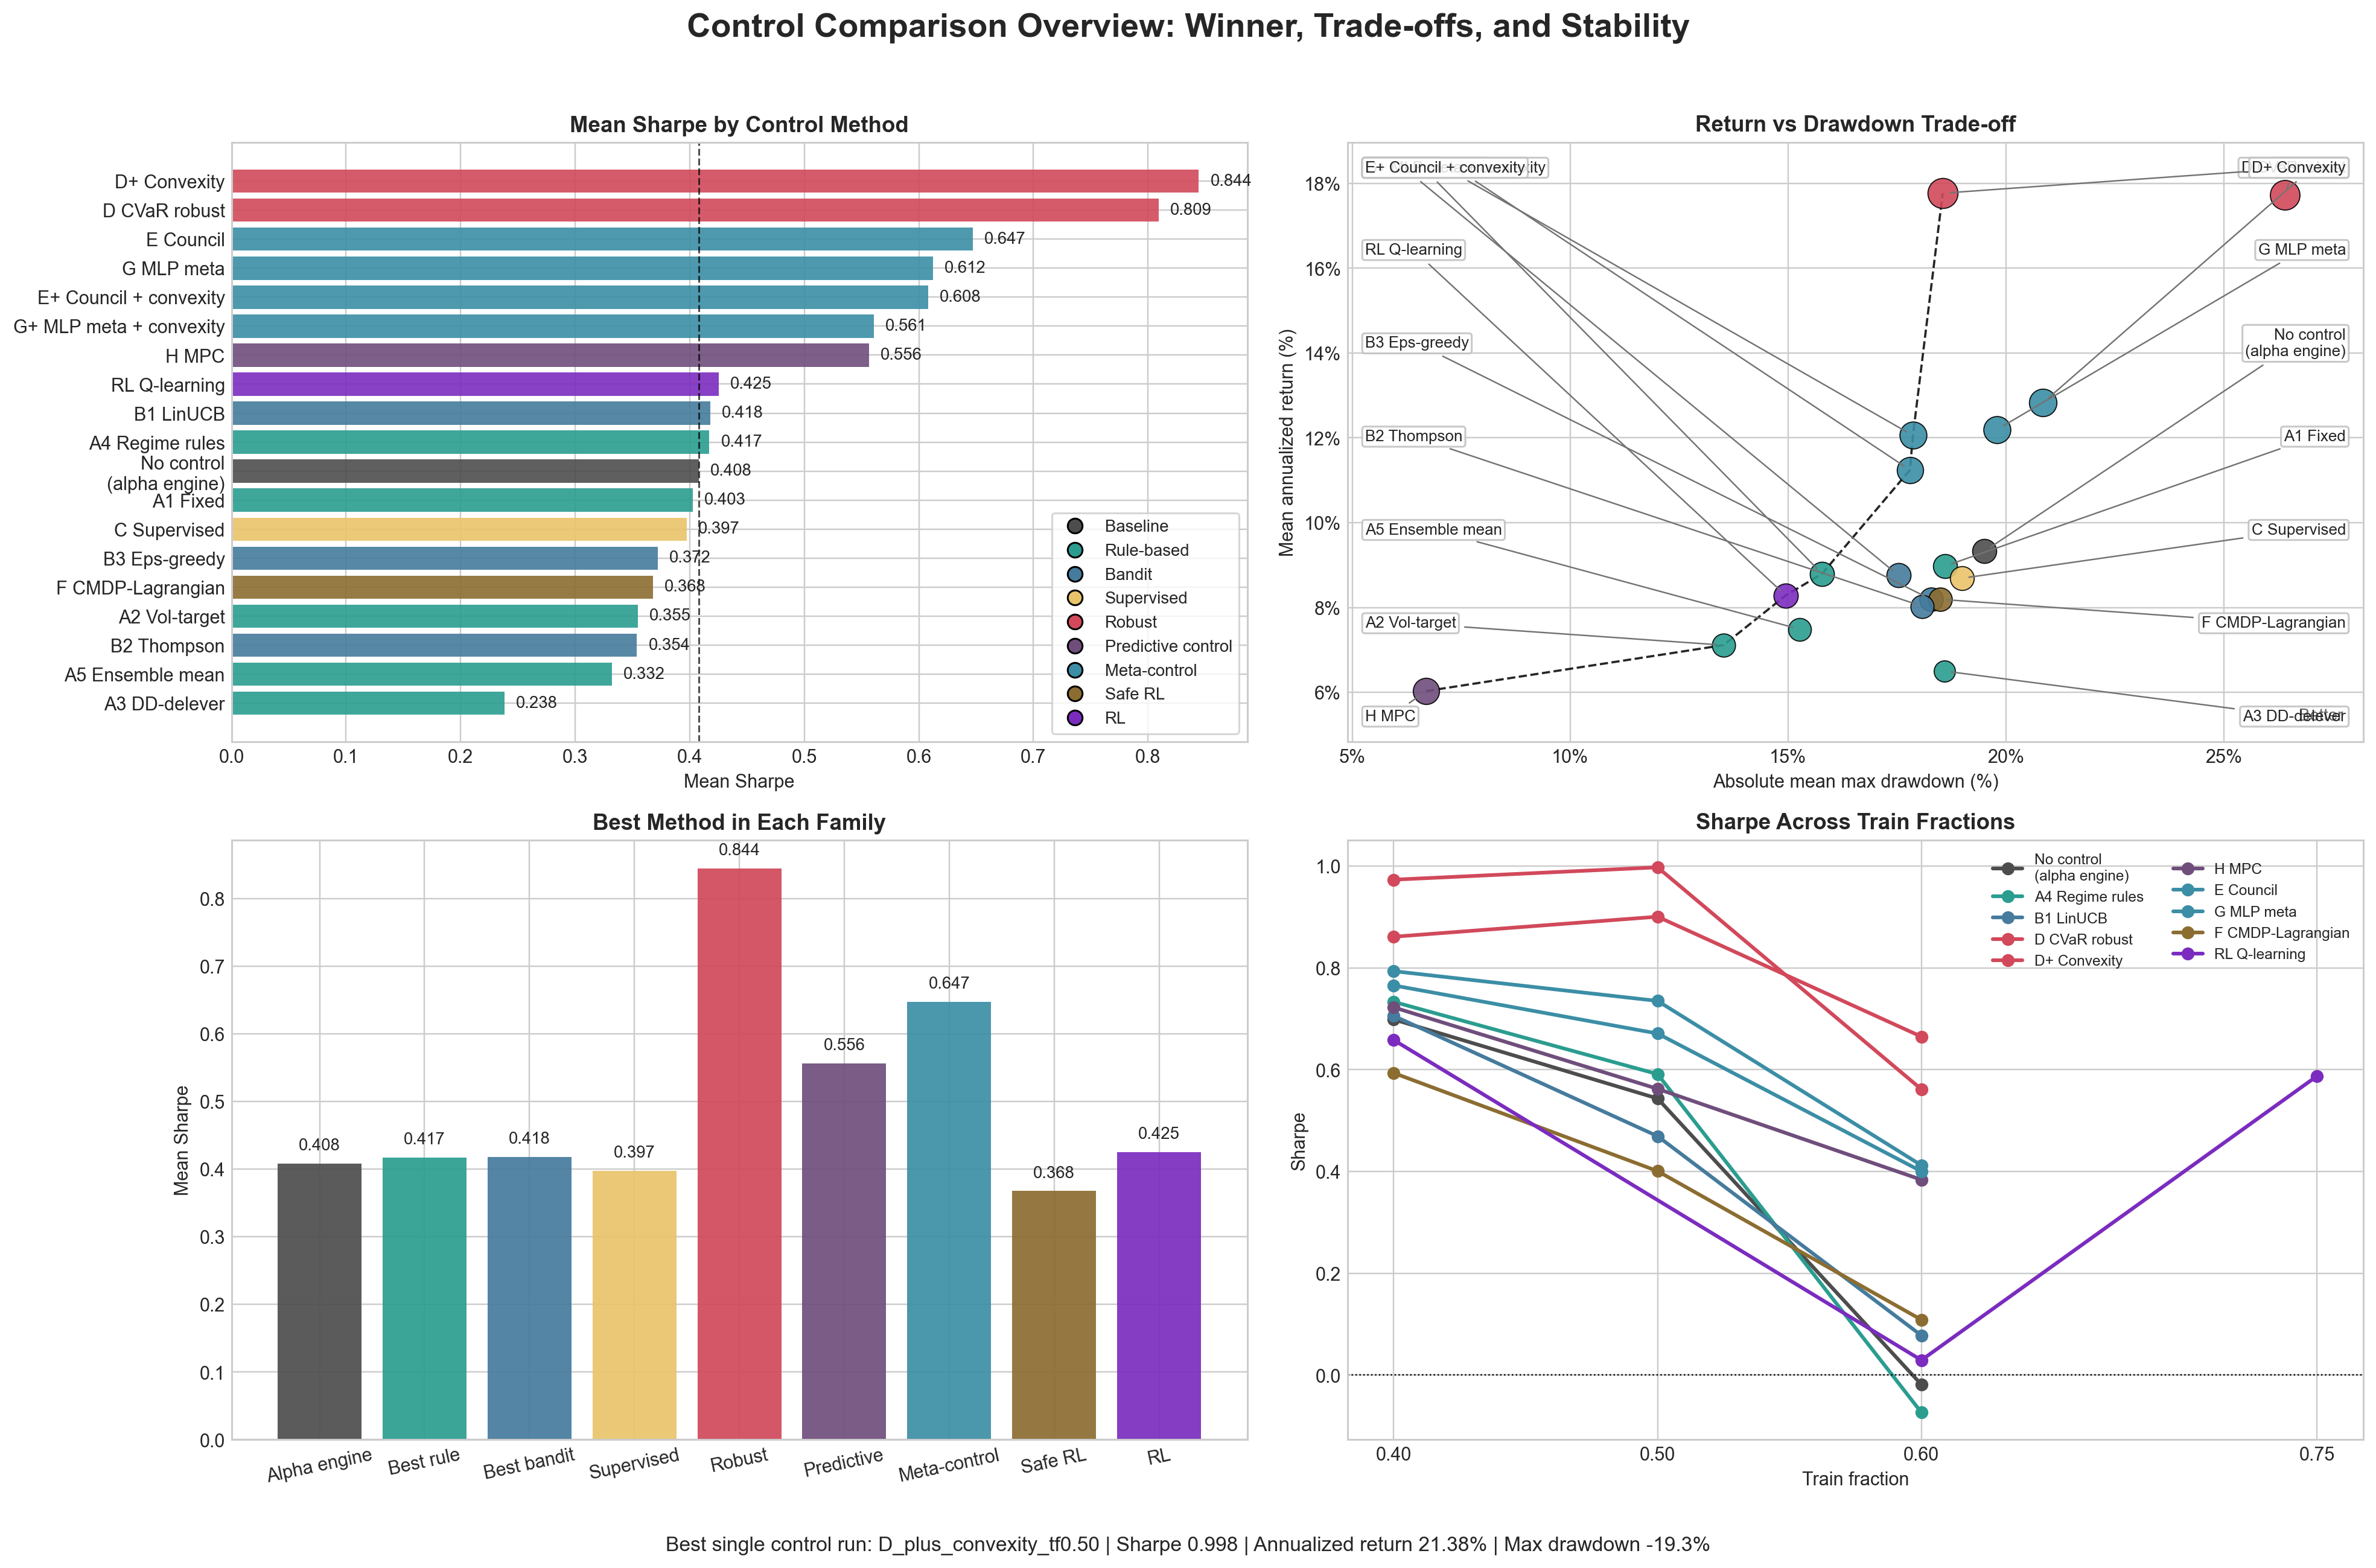
\includegraphics[width=\linewidth]{../../results/20260330_221820_universe_A/control_method_overview.png}
\end{minipage}\hfill
\begin{minipage}{0.49\textwidth}
\centering
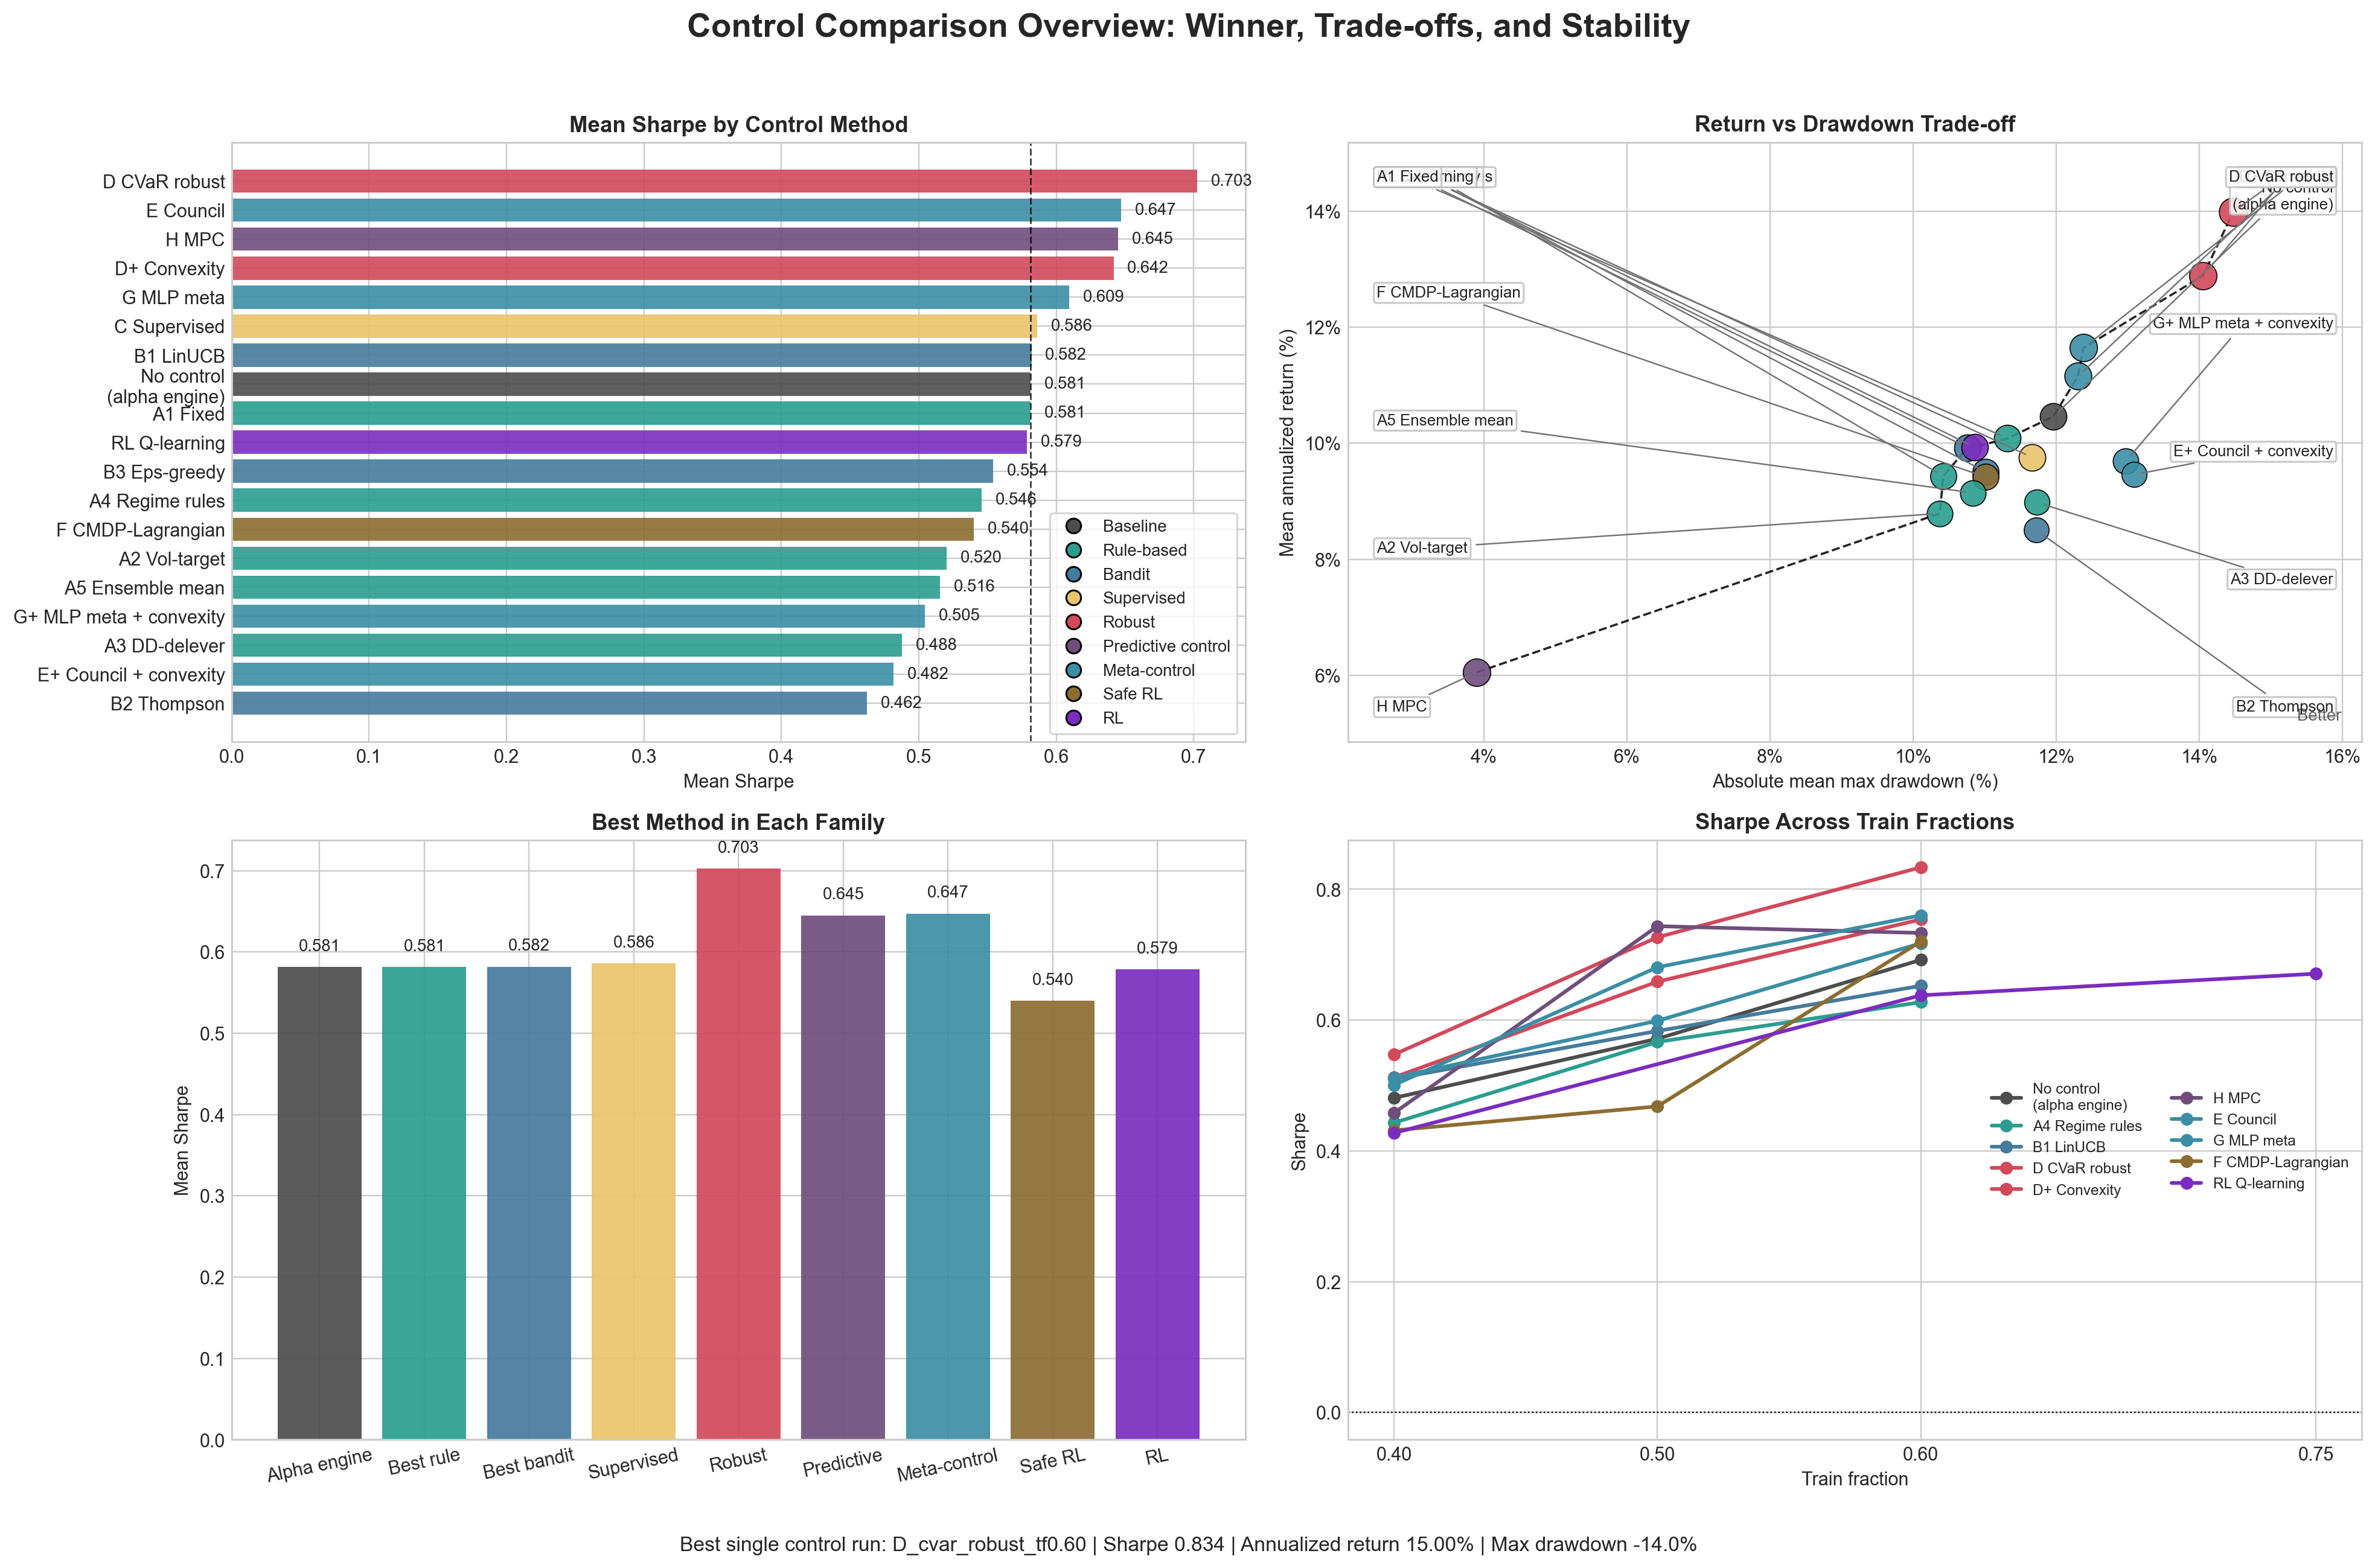
\includegraphics[width=\linewidth]{../../results/20260331_002747_universe_B/control_method_overview.png}
\end{minipage}
\caption{Control-method overview plots for the two archived universes. Left:
Universe A, where \texttt{D\_plus\_convexity} is the flagship performer.
Right: Universe B, where the robust frontier is tighter and plain
\texttt{D\_cvar\_robust} leads on mean Sharpe.}
\label{fig:control_overview}
\end{figure*}
}{}

\IfFileExists{../../results/20260330_221820_universe_A/control_split_heatmaps.png}{
\begin{figure*}[p]
\centering
\begin{minipage}{0.49\textwidth}
\centering
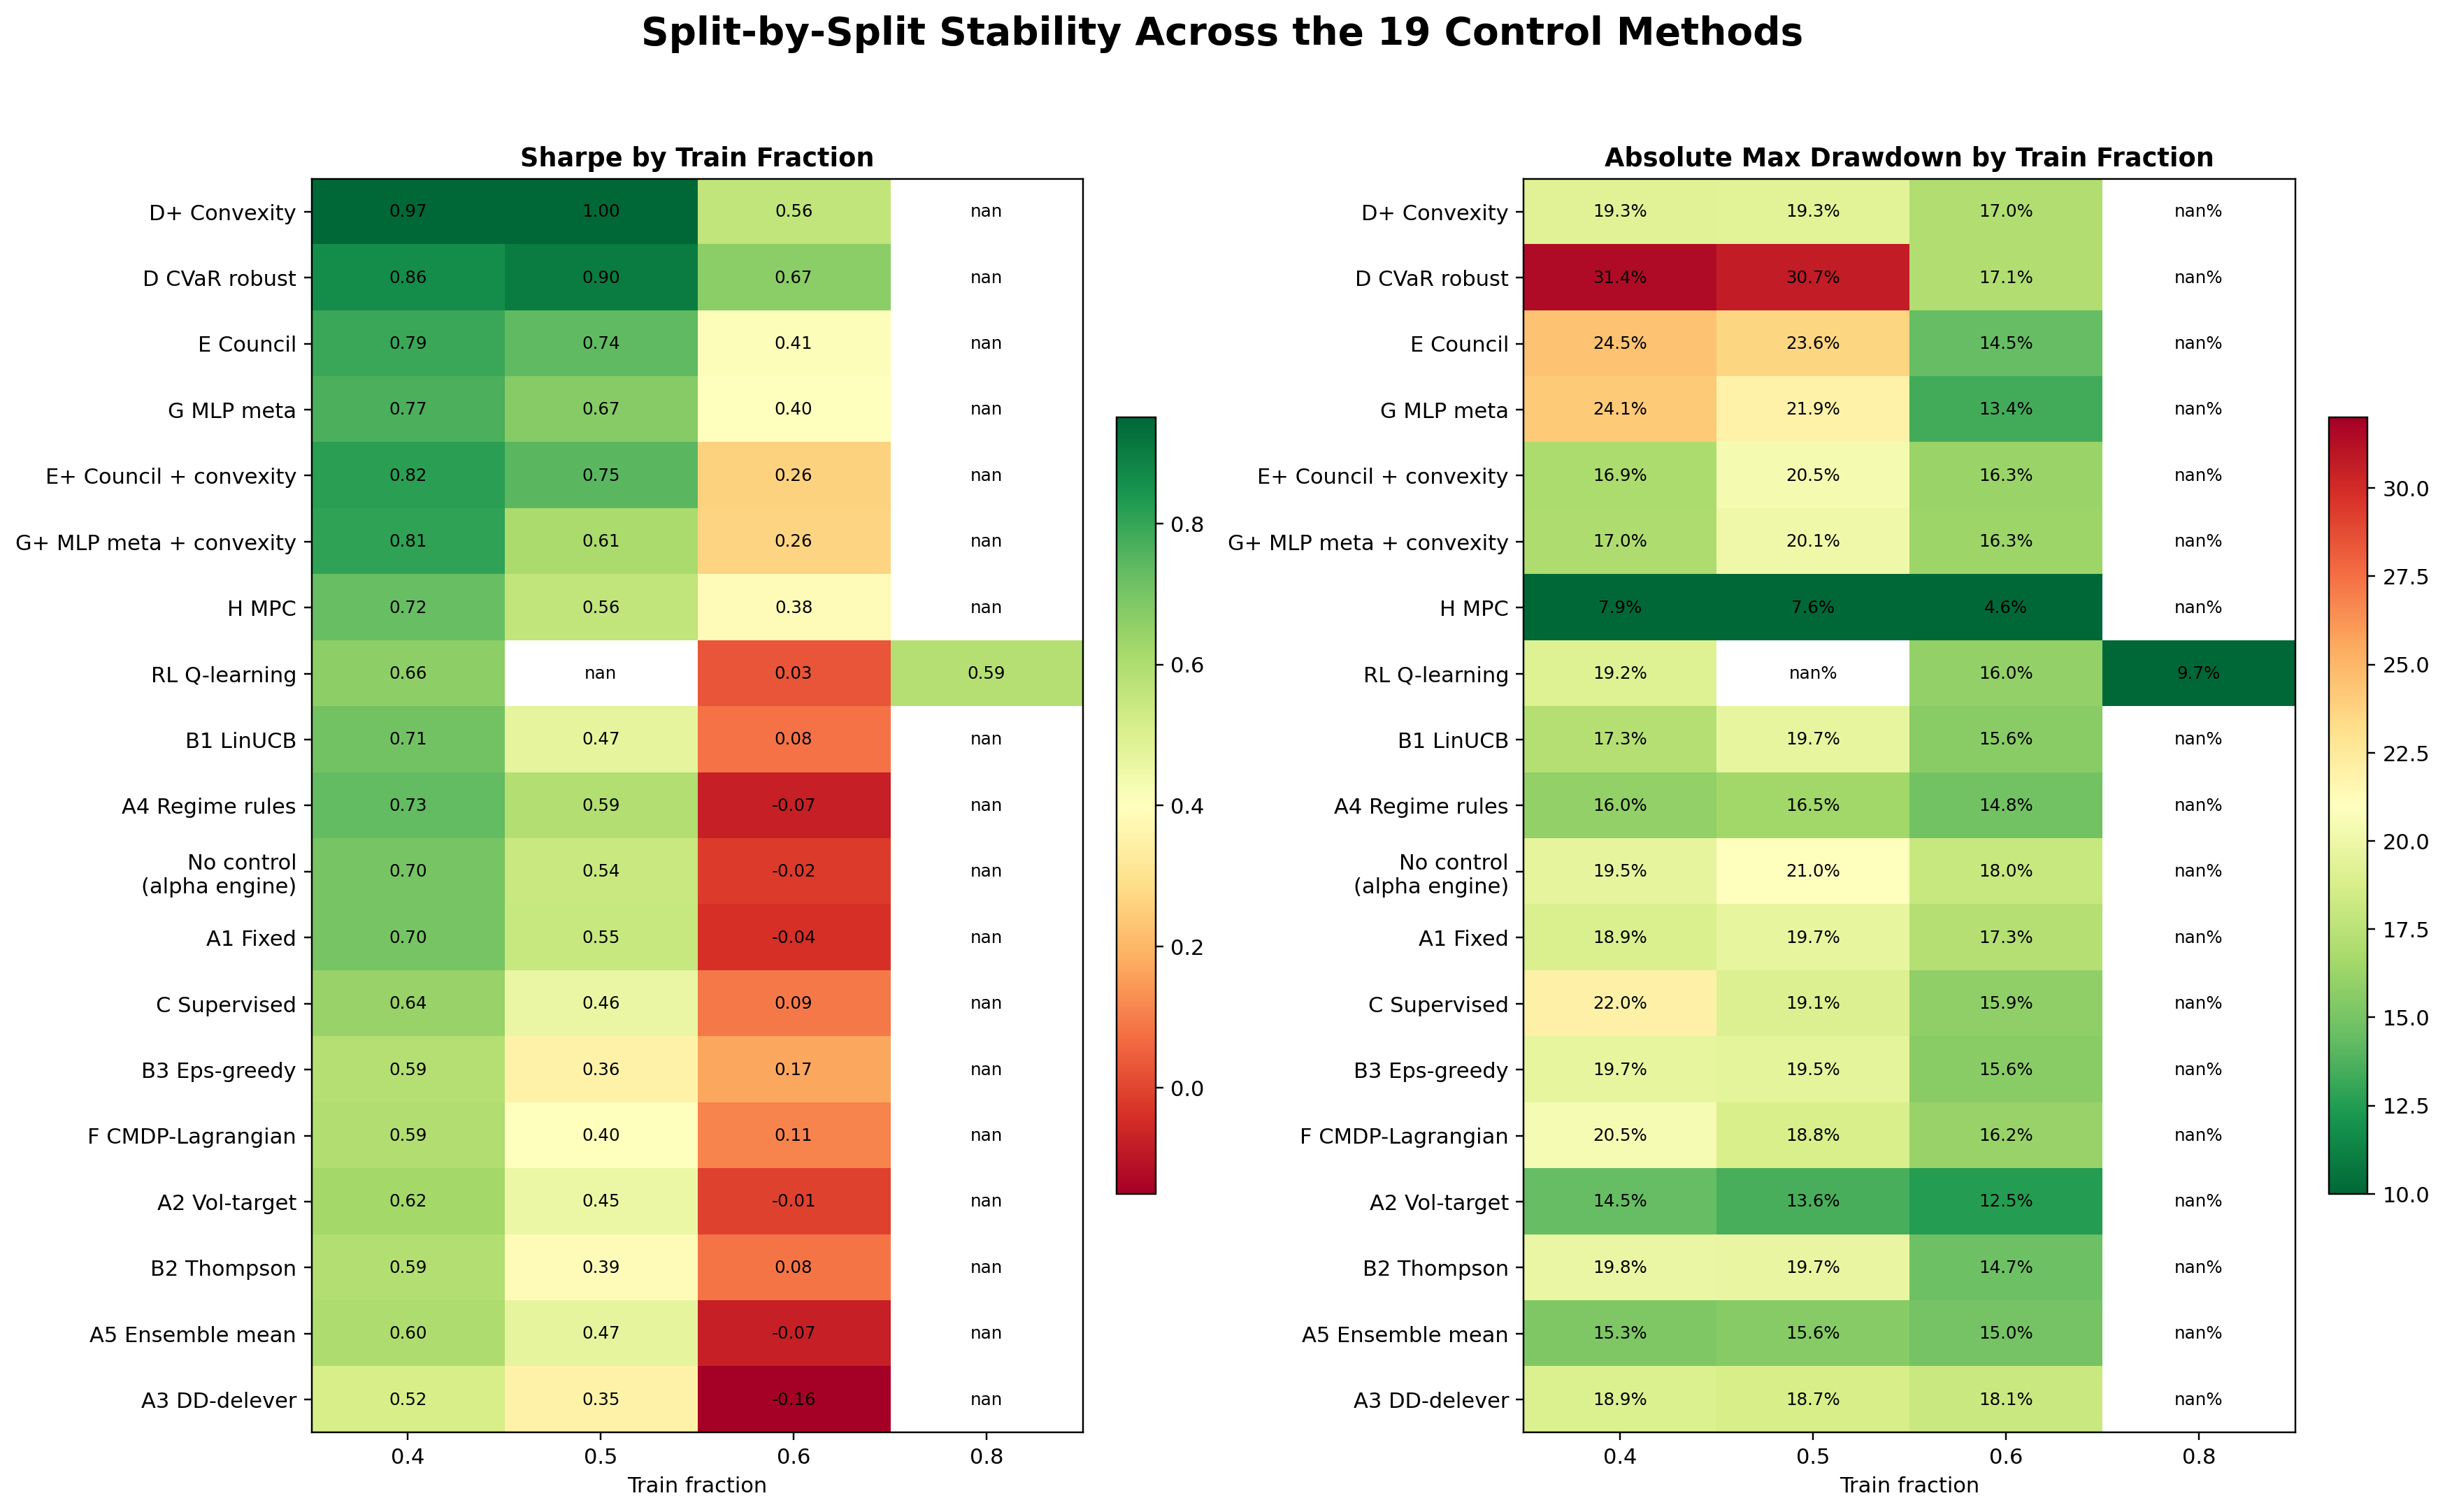
\includegraphics[width=\linewidth]{../../results/20260330_221820_universe_A/control_split_heatmaps.png}
\end{minipage}\hfill
\begin{minipage}{0.49\textwidth}
\centering
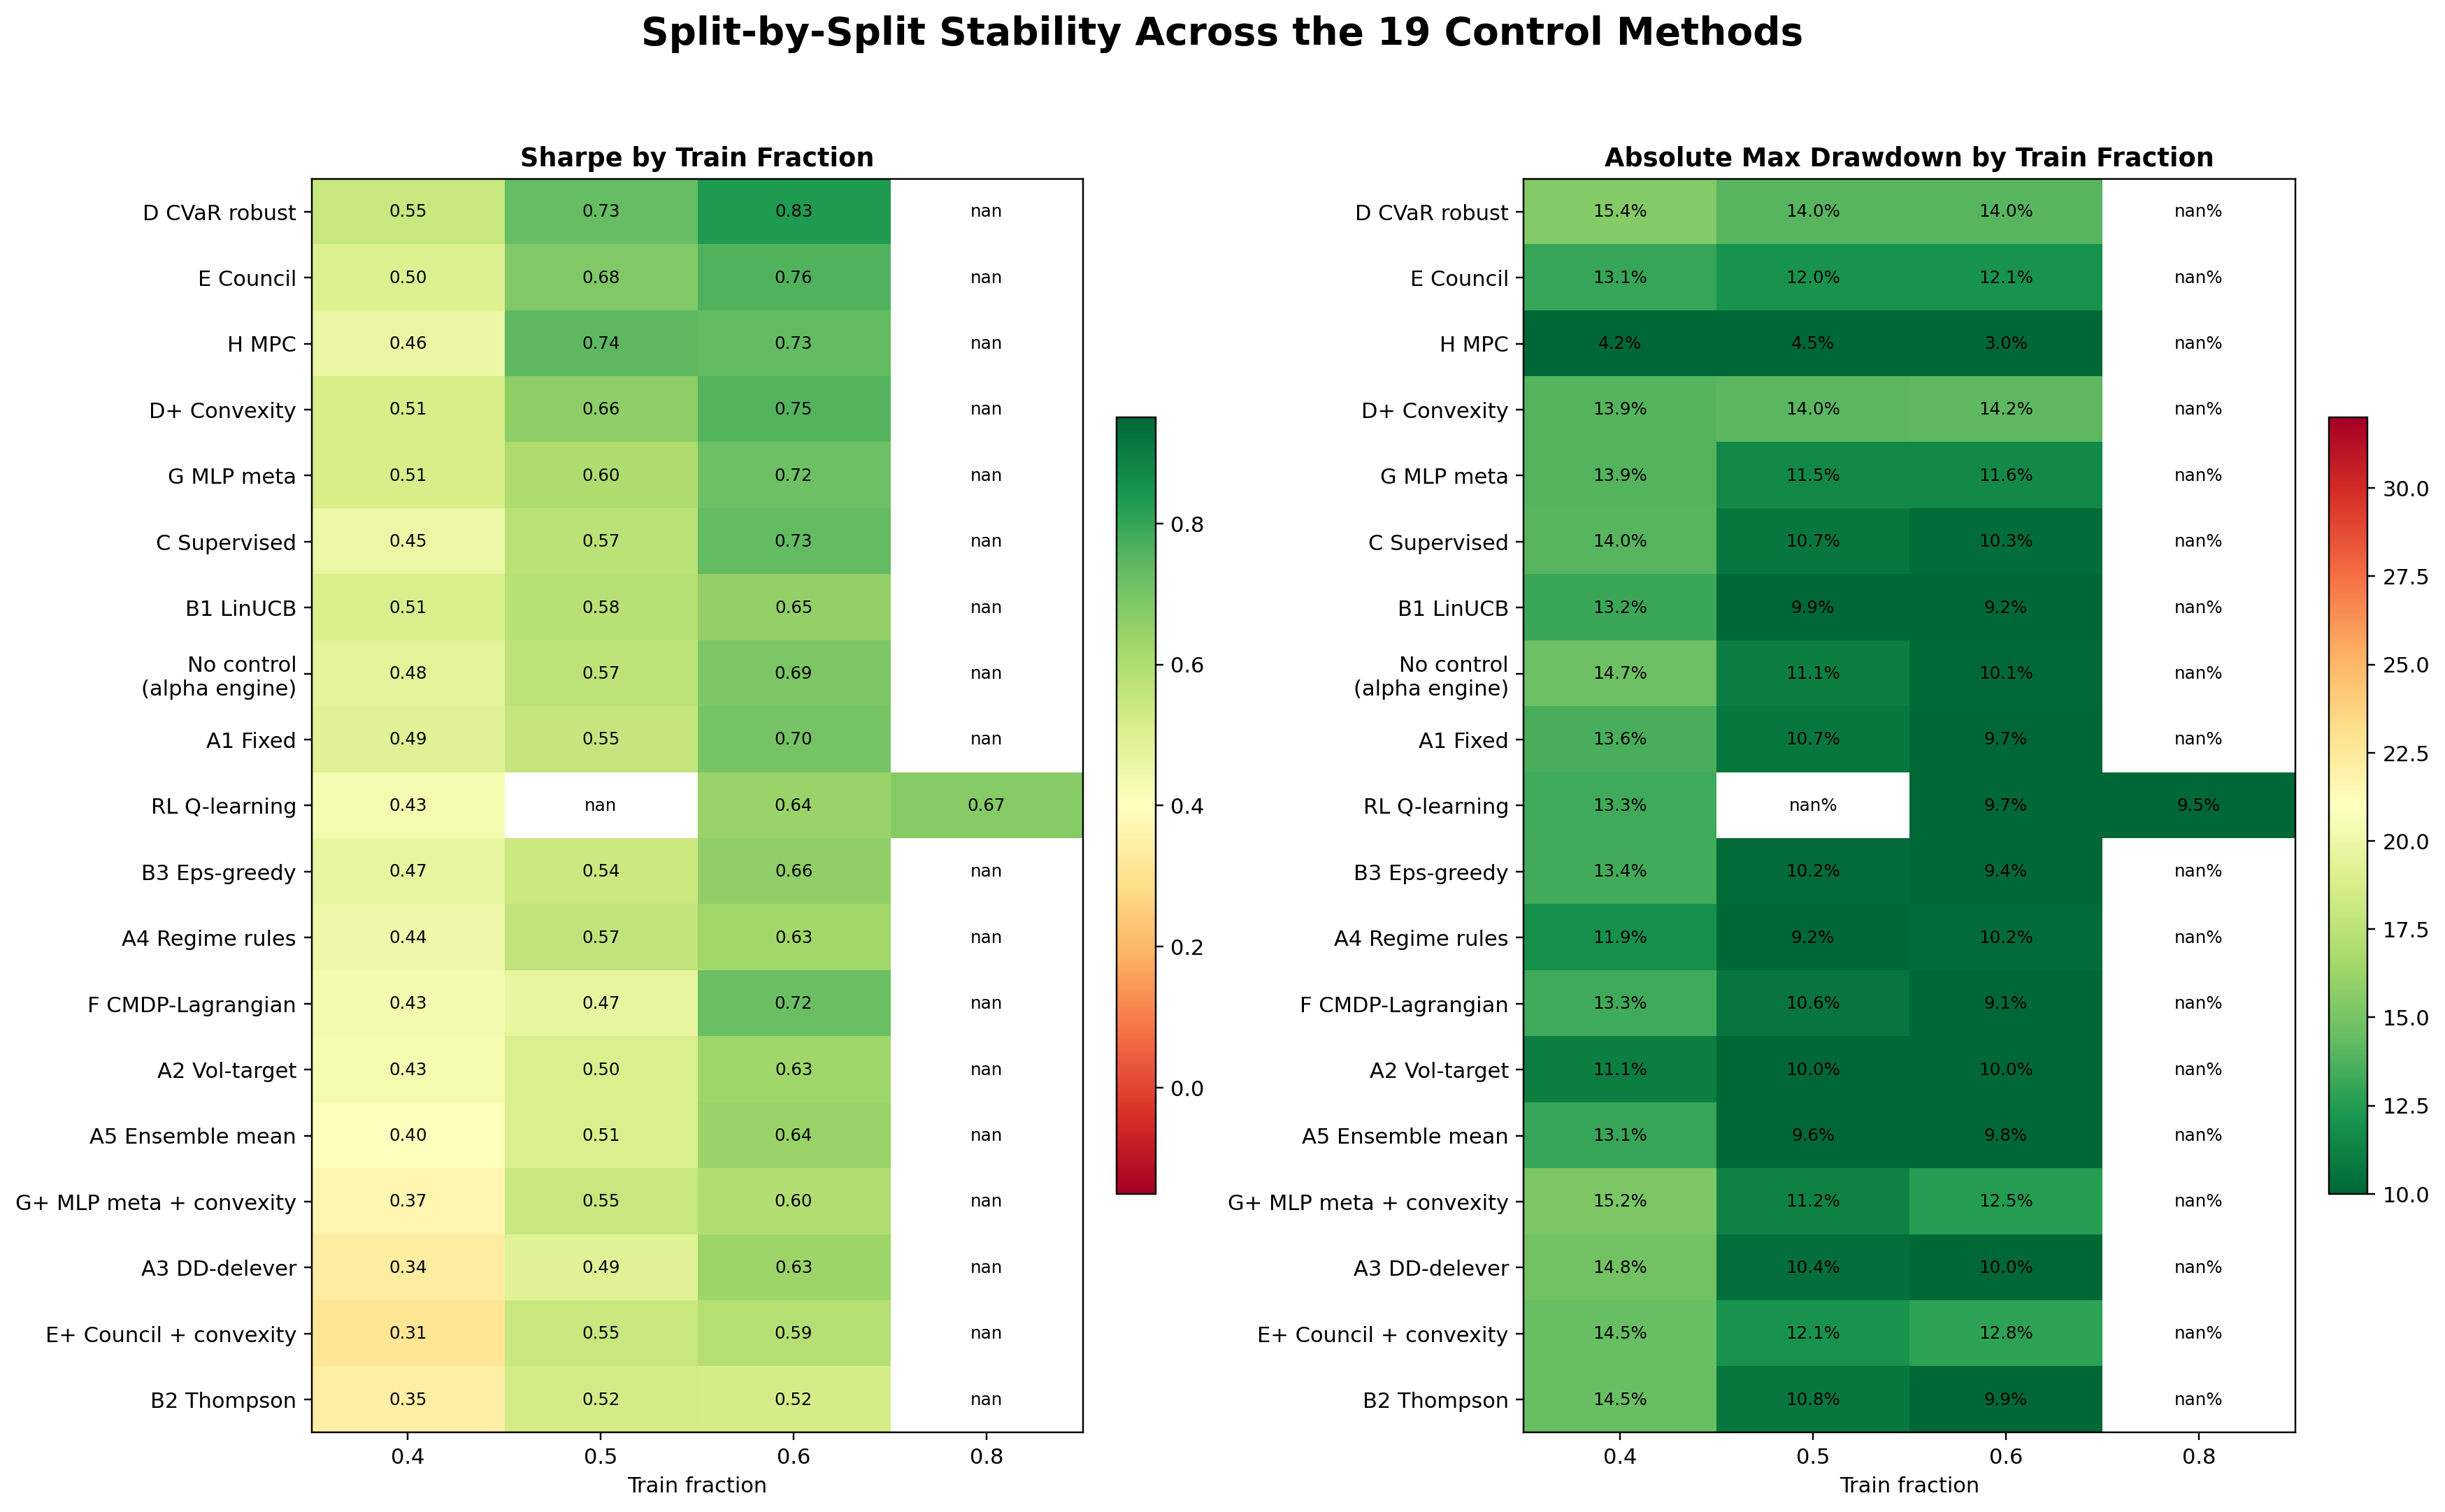
\includegraphics[width=\linewidth]{../../results/20260331_002747_universe_B/control_split_heatmaps.png}
\end{minipage}
\caption{Split-stability heatmaps for the control-comparison suite in the two
universes. These plots summarize how controller rankings change across the
three train-fraction splits.}
\label{fig:split_heatmaps}
\end{figure*}
}{}

\IfFileExists{../../results/20260330_221820_universe_A/control_pareto_frontier.png}{
\begin{figure*}[p]
\centering
\begin{minipage}{0.49\textwidth}
\centering
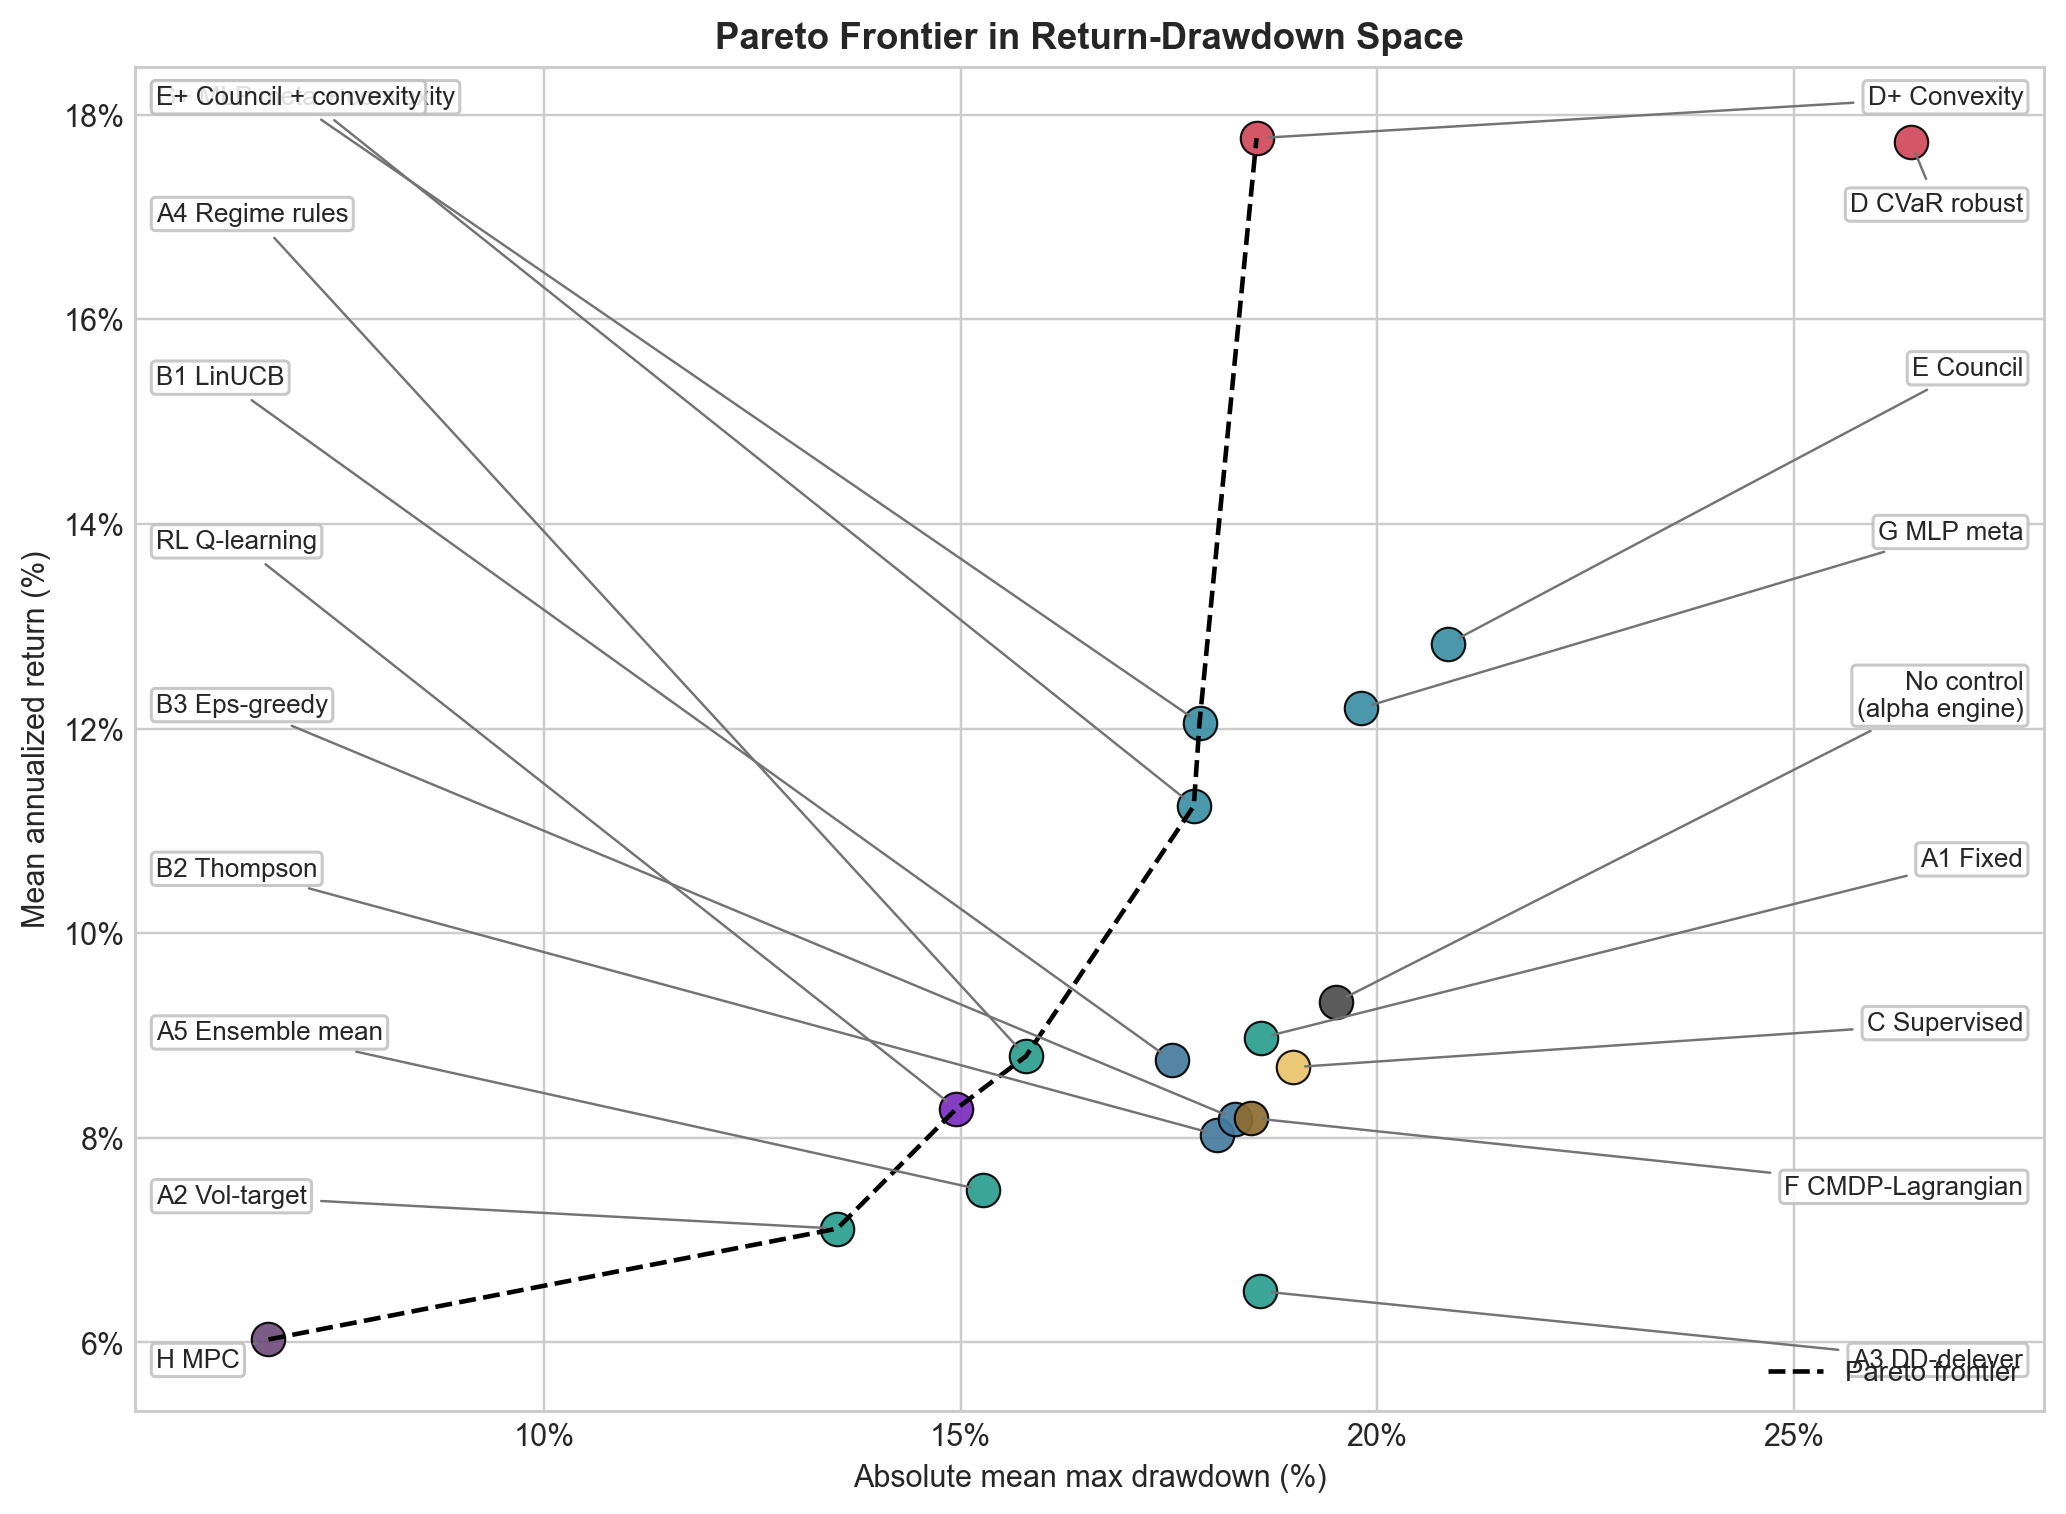
\includegraphics[width=\linewidth]{../../results/20260330_221820_universe_A/control_pareto_frontier.png}
\end{minipage}\hfill
\begin{minipage}{0.49\textwidth}
\centering
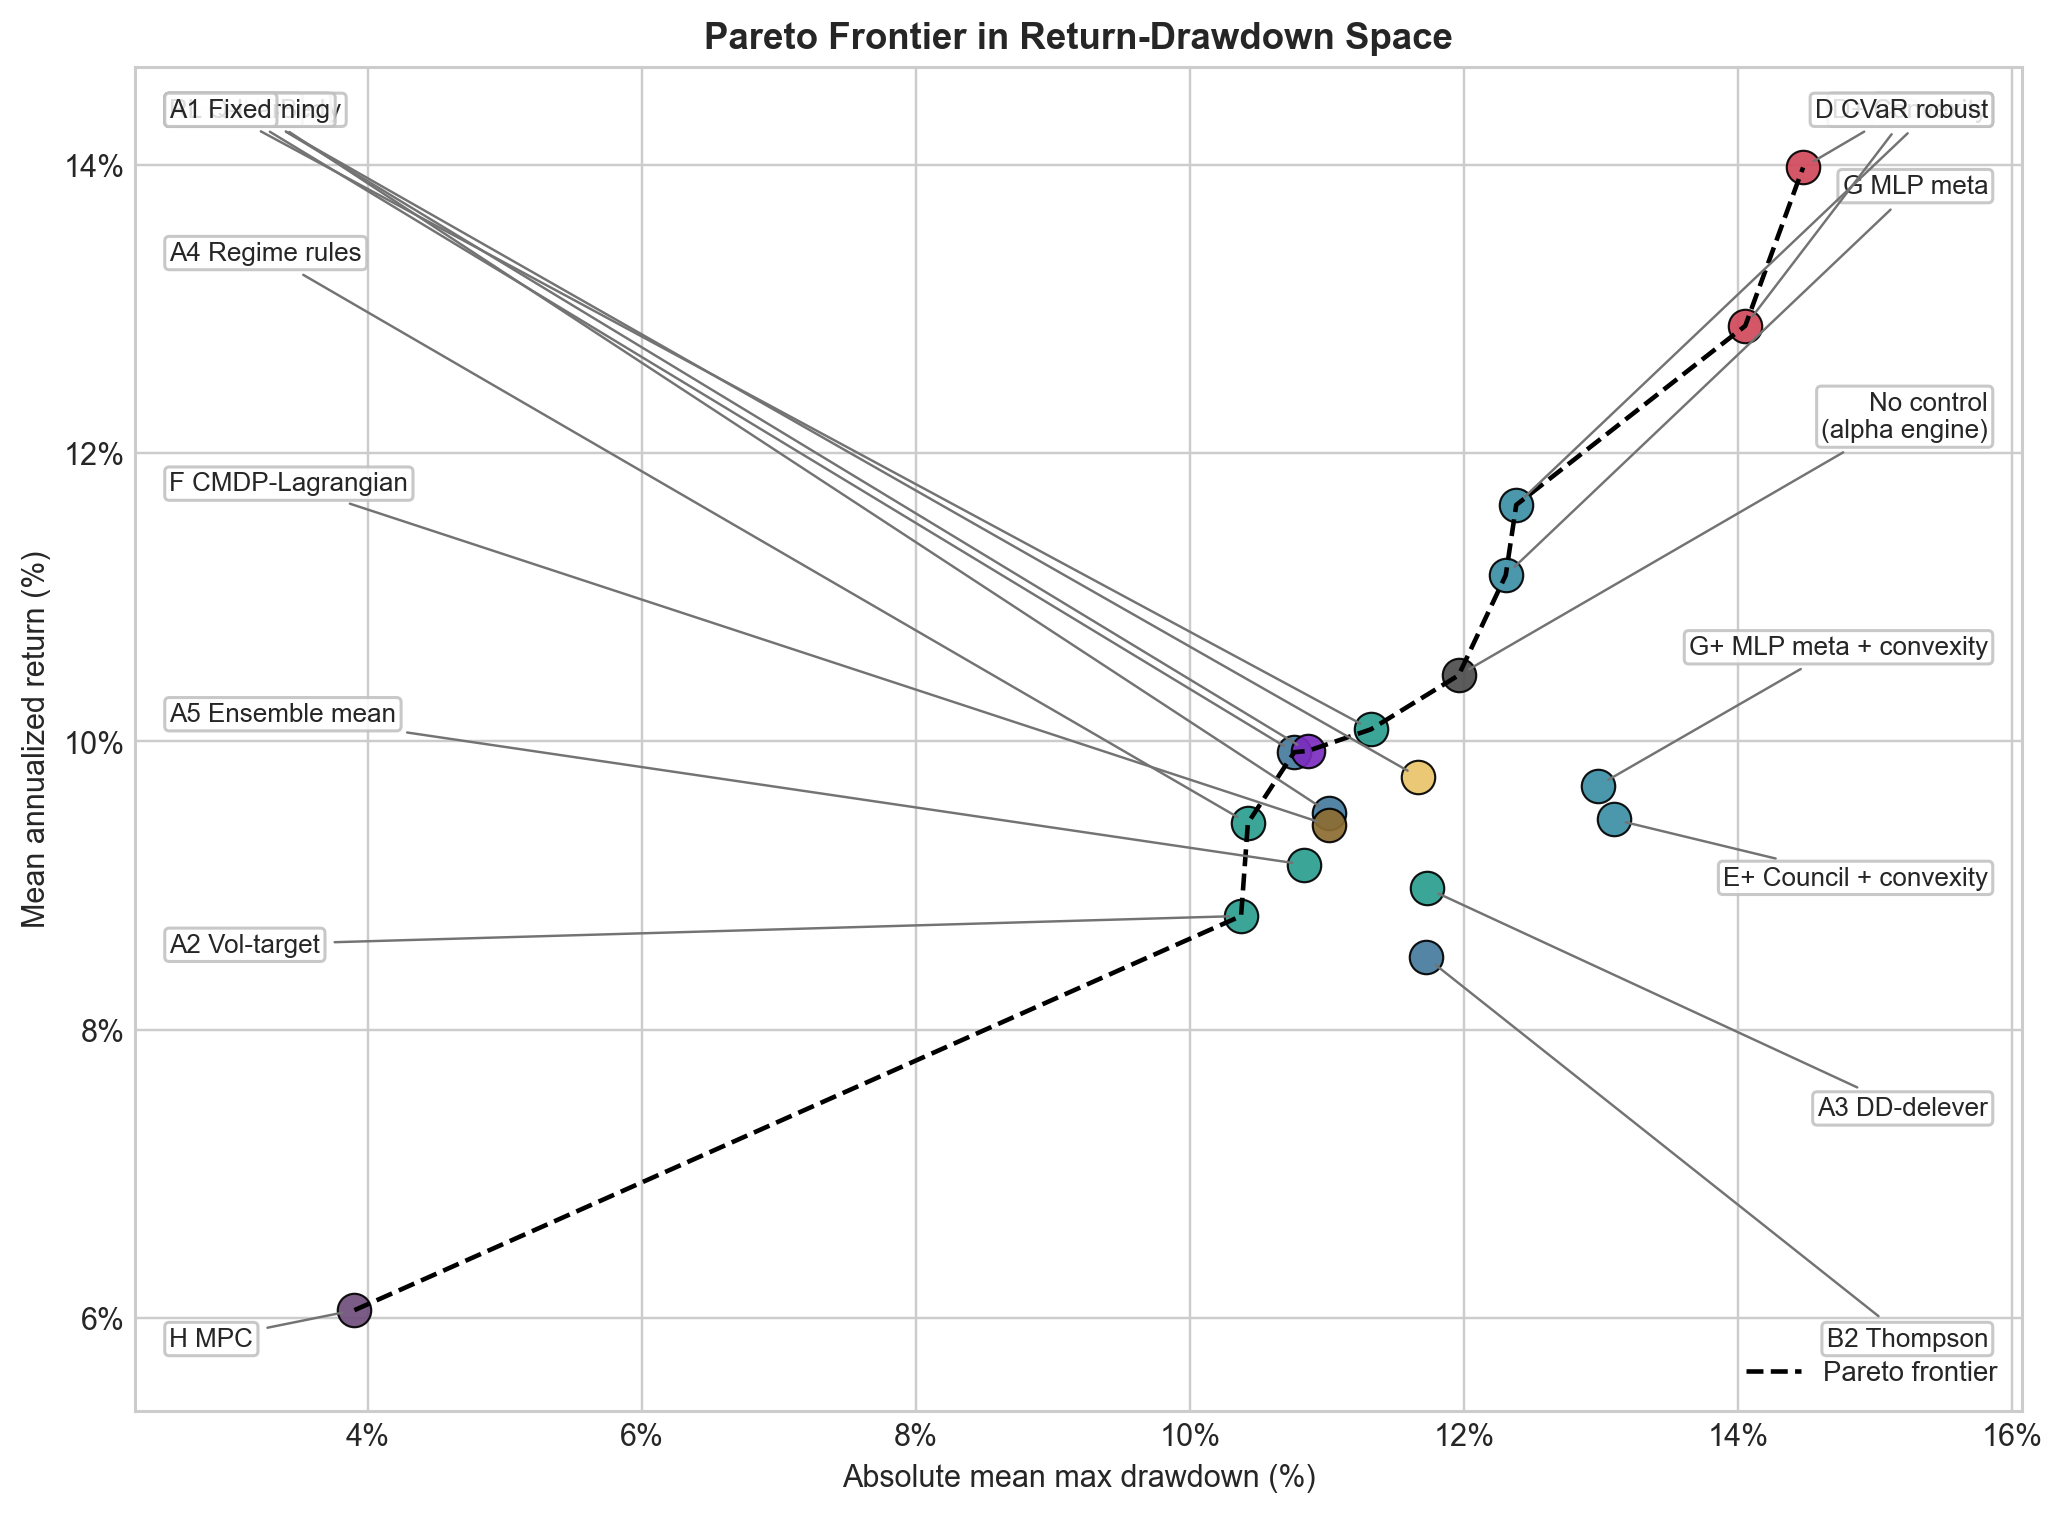
\includegraphics[width=\linewidth]{../../results/20260331_002747_universe_B/control_pareto_frontier.png}
\end{minipage}
\caption{Pareto frontiers in return--drawdown space for the two archived
universes. Universe A shows the strongest outward push from
\texttt{D\_plus\_convexity}; Universe B is tighter, with plain
\texttt{D\_cvar\_robust}, \texttt{E\_council}, and \texttt{H\_mpc} clustering
near the defensive frontier.}
\label{fig:control_heatmaps}
\end{figure*}
}{}

\IfFileExists{../../results/20260330_221820_universe_A/control_interpretability.png}{
\begin{figure*}[p]
\centering
\begin{minipage}{0.49\textwidth}
\centering
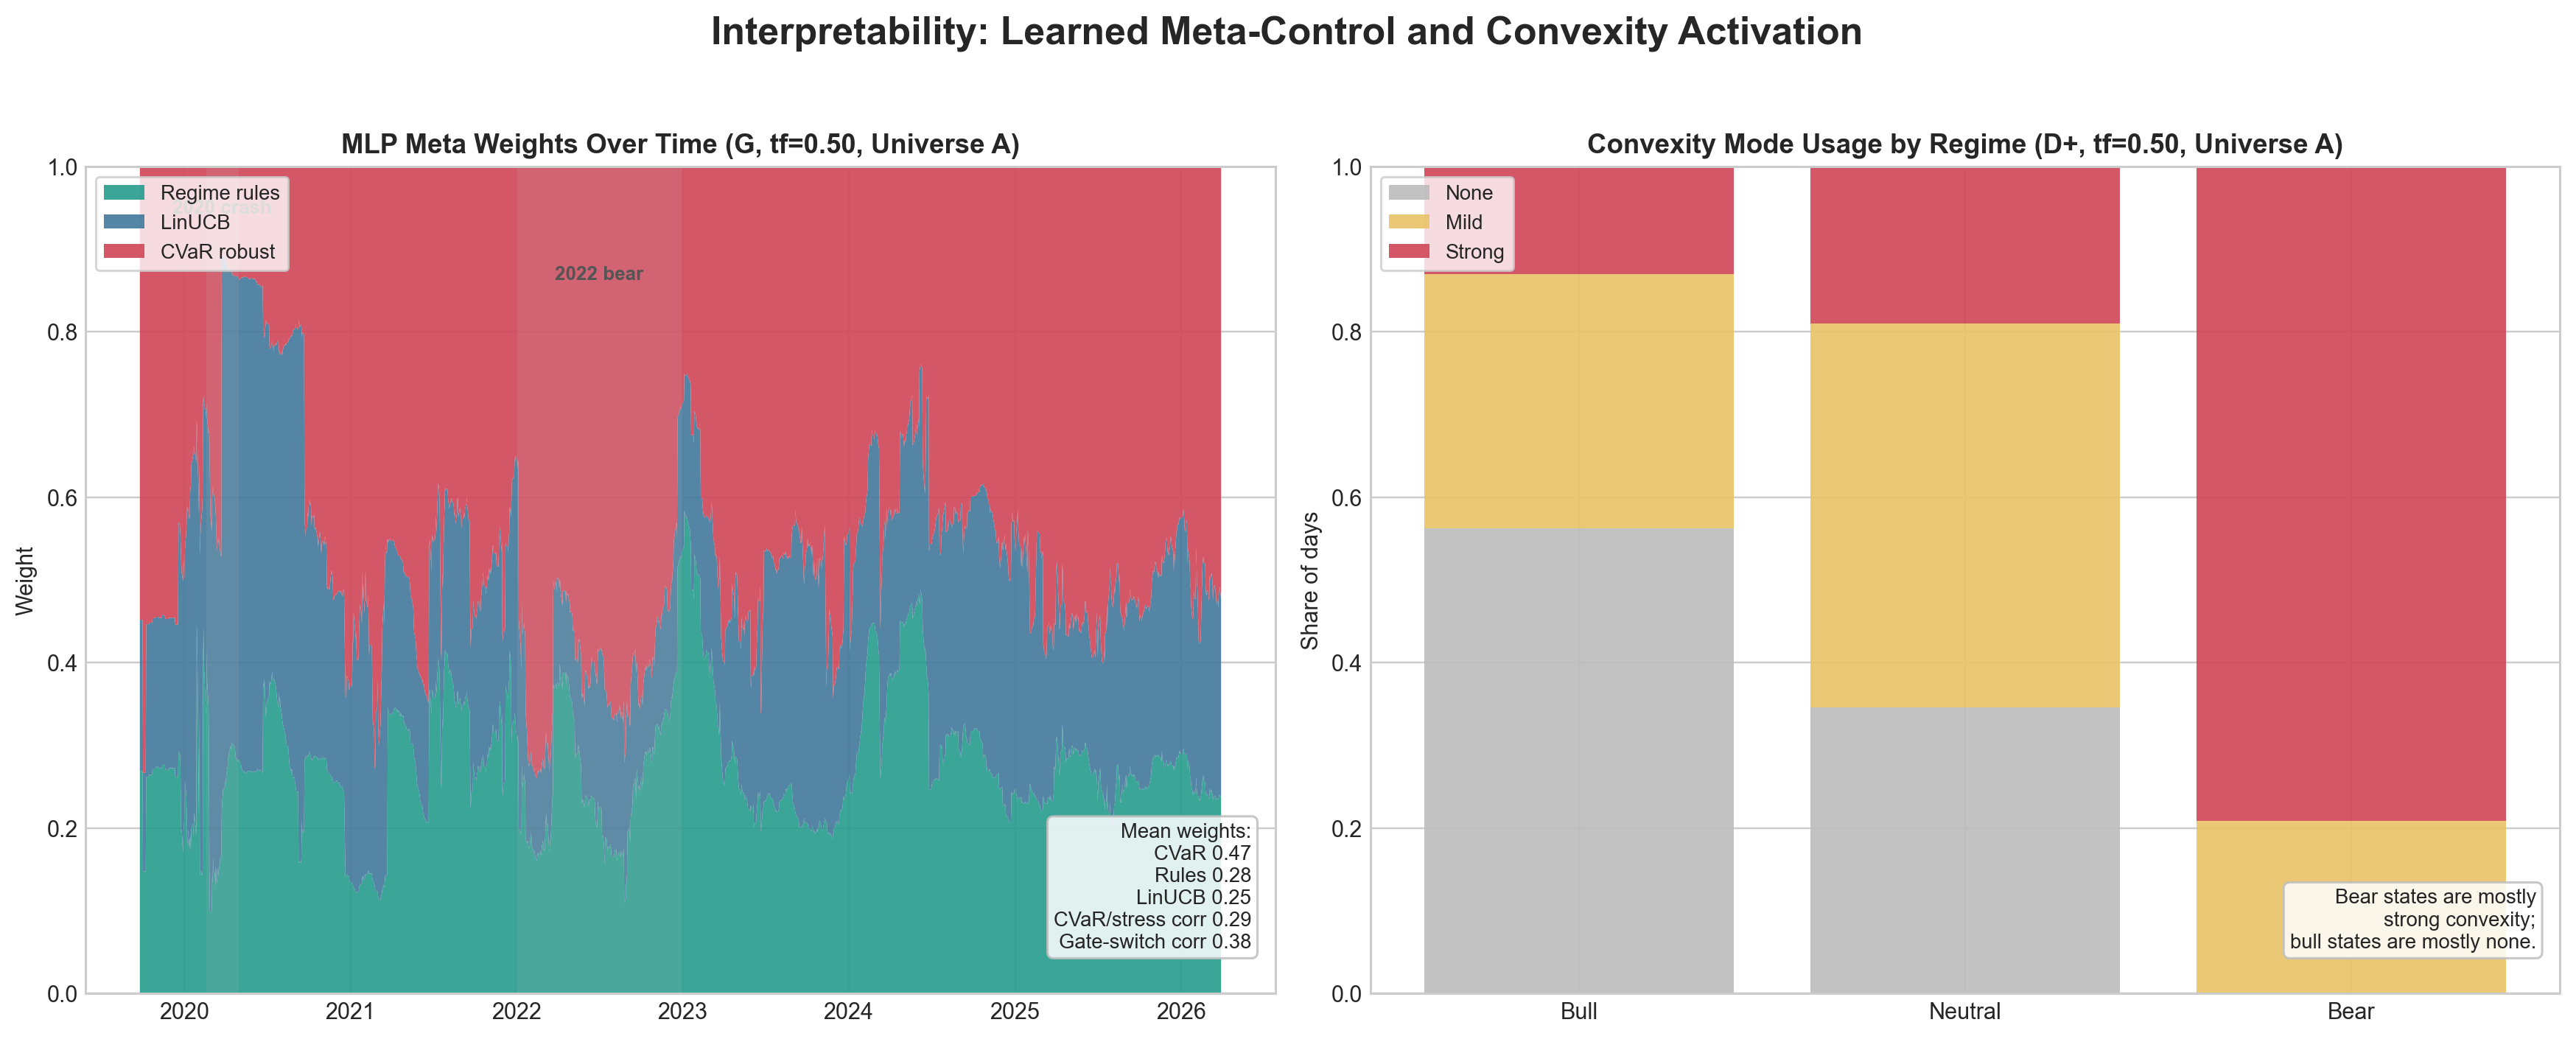
\includegraphics[width=\linewidth]{../../results/20260330_221820_universe_A/control_interpretability.png}
\end{minipage}\hfill
\begin{minipage}{0.49\textwidth}
\centering
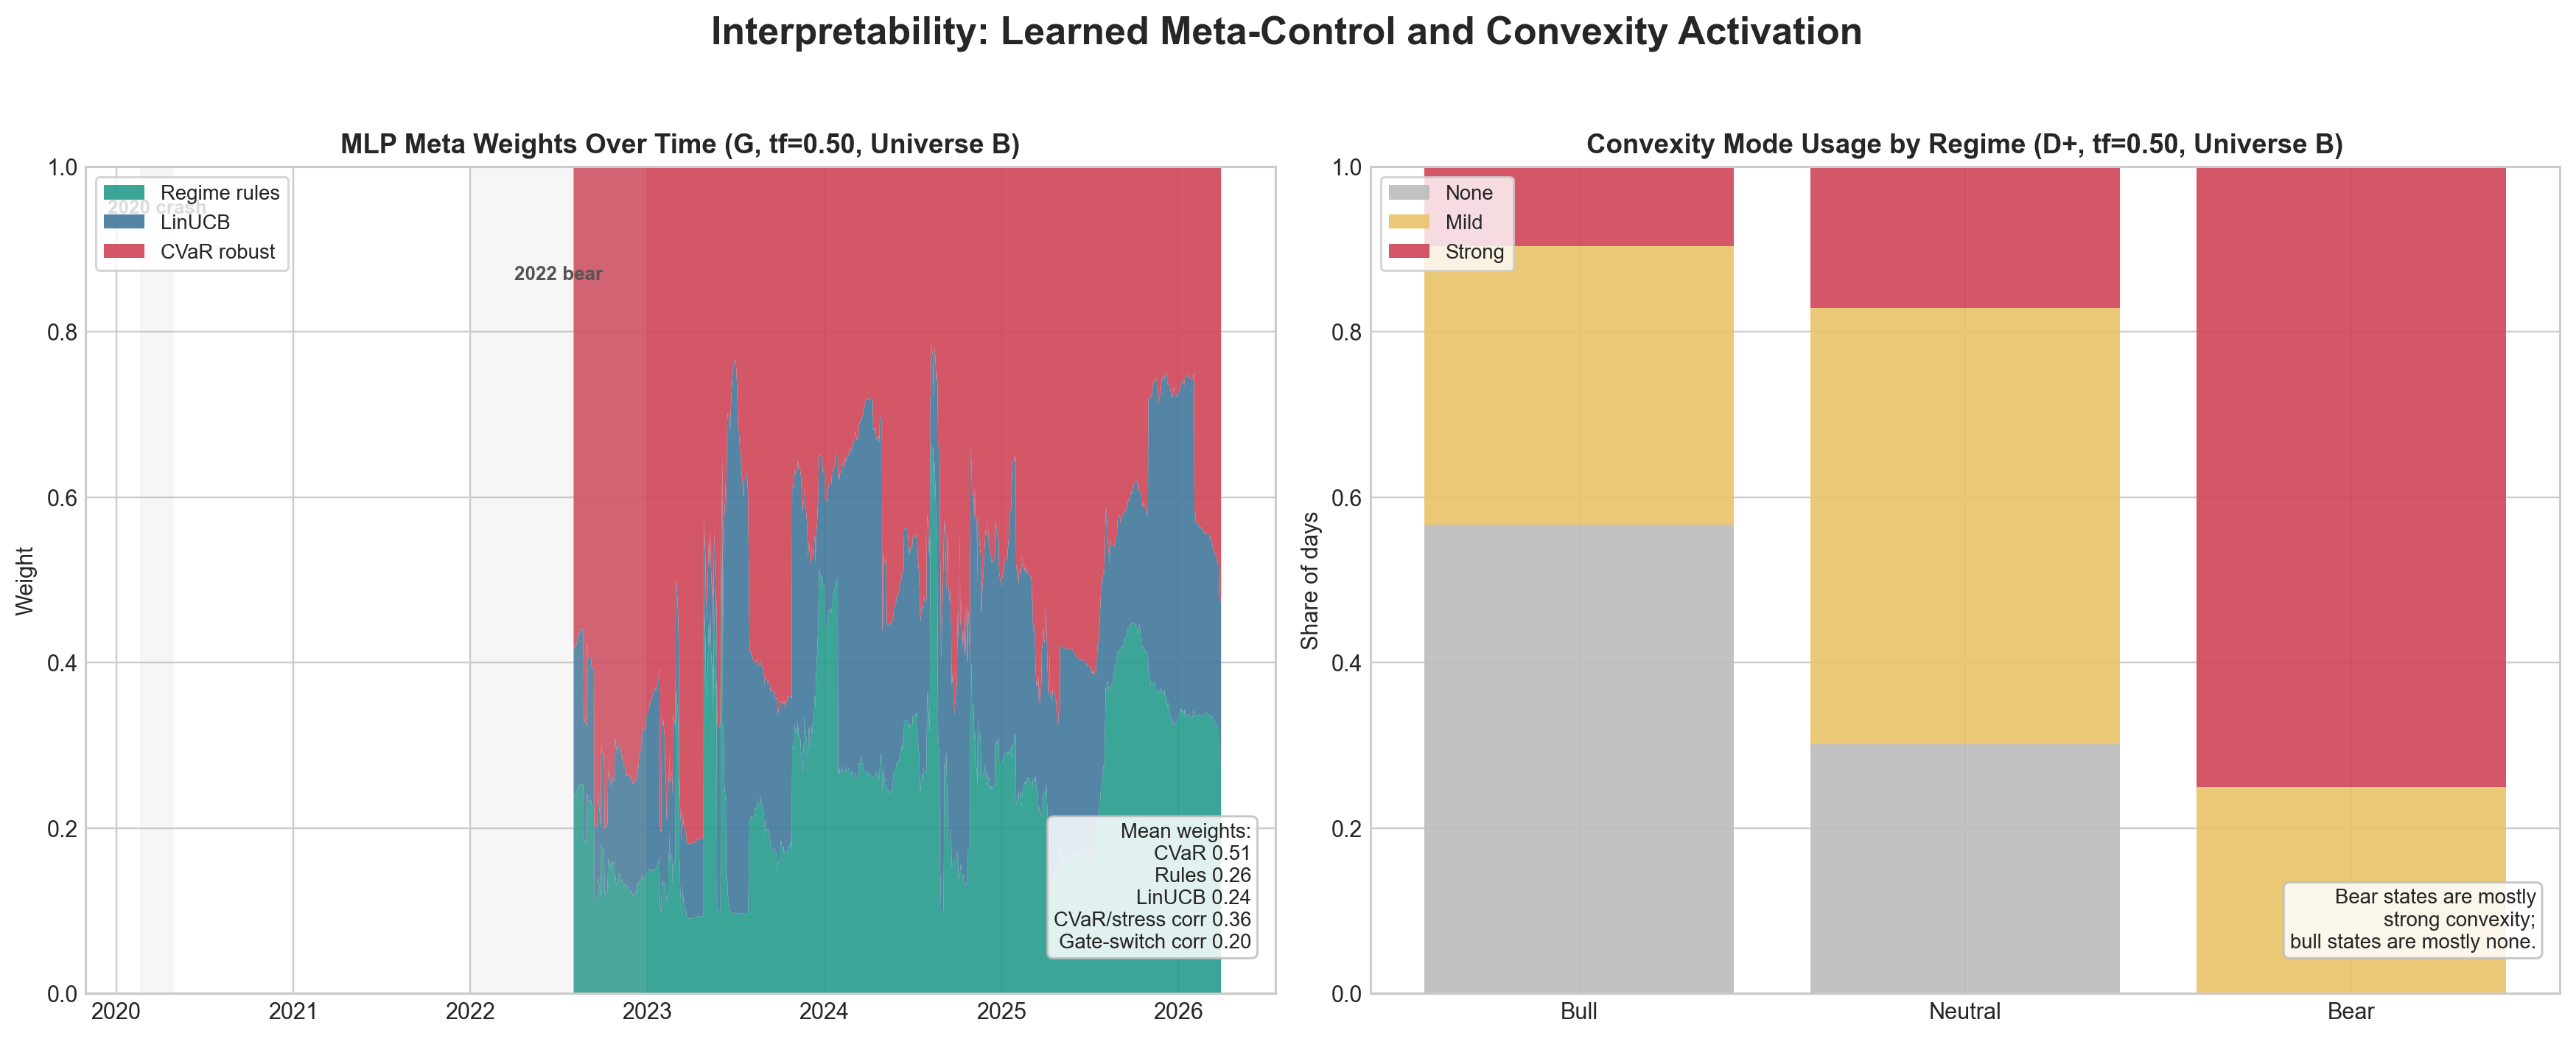
\includegraphics[width=\linewidth]{../../results/20260331_002747_universe_B/control_interpretability.png}
\end{minipage}
\caption{Interpretability diagnostics for the reference split in both
universes. The left panel in each image shows how the learned gate reallocates
weight across experts through time; the right panel shows convexity mode usage
by regime.}
\label{fig:interpretability}
\end{figure*}
}{}

\IfFileExists{../../results/20260330_221820_universe_A/control_tail_diagnostic.png}{
\begin{figure*}[p]
\centering
\begin{minipage}{0.49\textwidth}
\centering
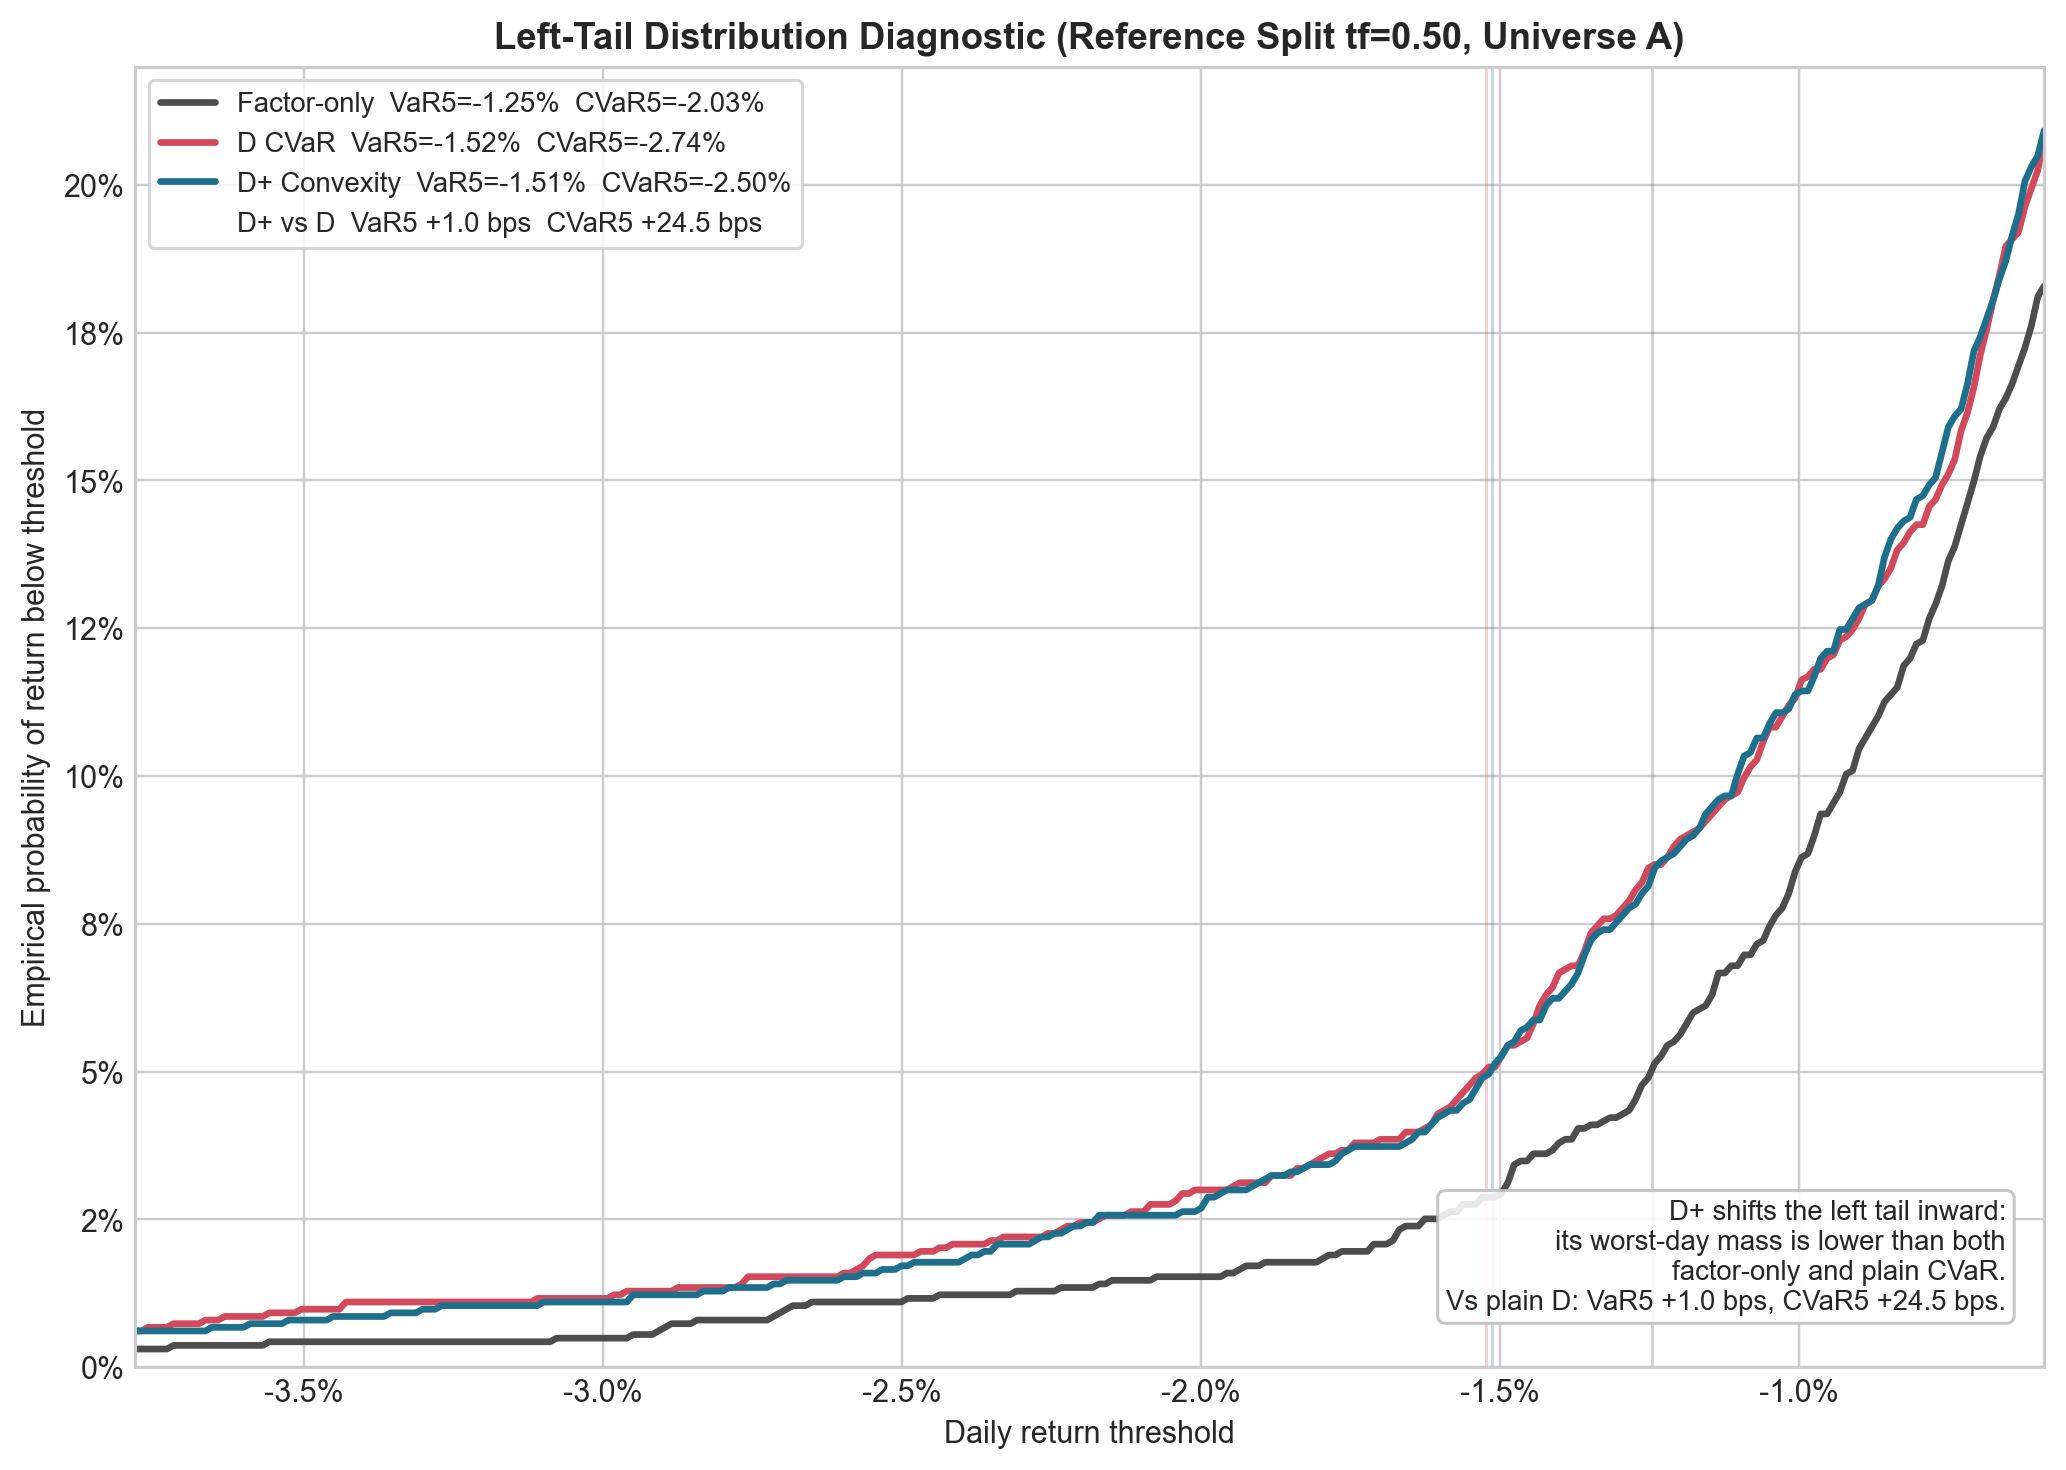
\includegraphics[width=0.95\linewidth]{../../results/20260330_221820_universe_A/control_tail_diagnostic.png}
\end{minipage}\hfill
\begin{minipage}{0.49\textwidth}
\centering
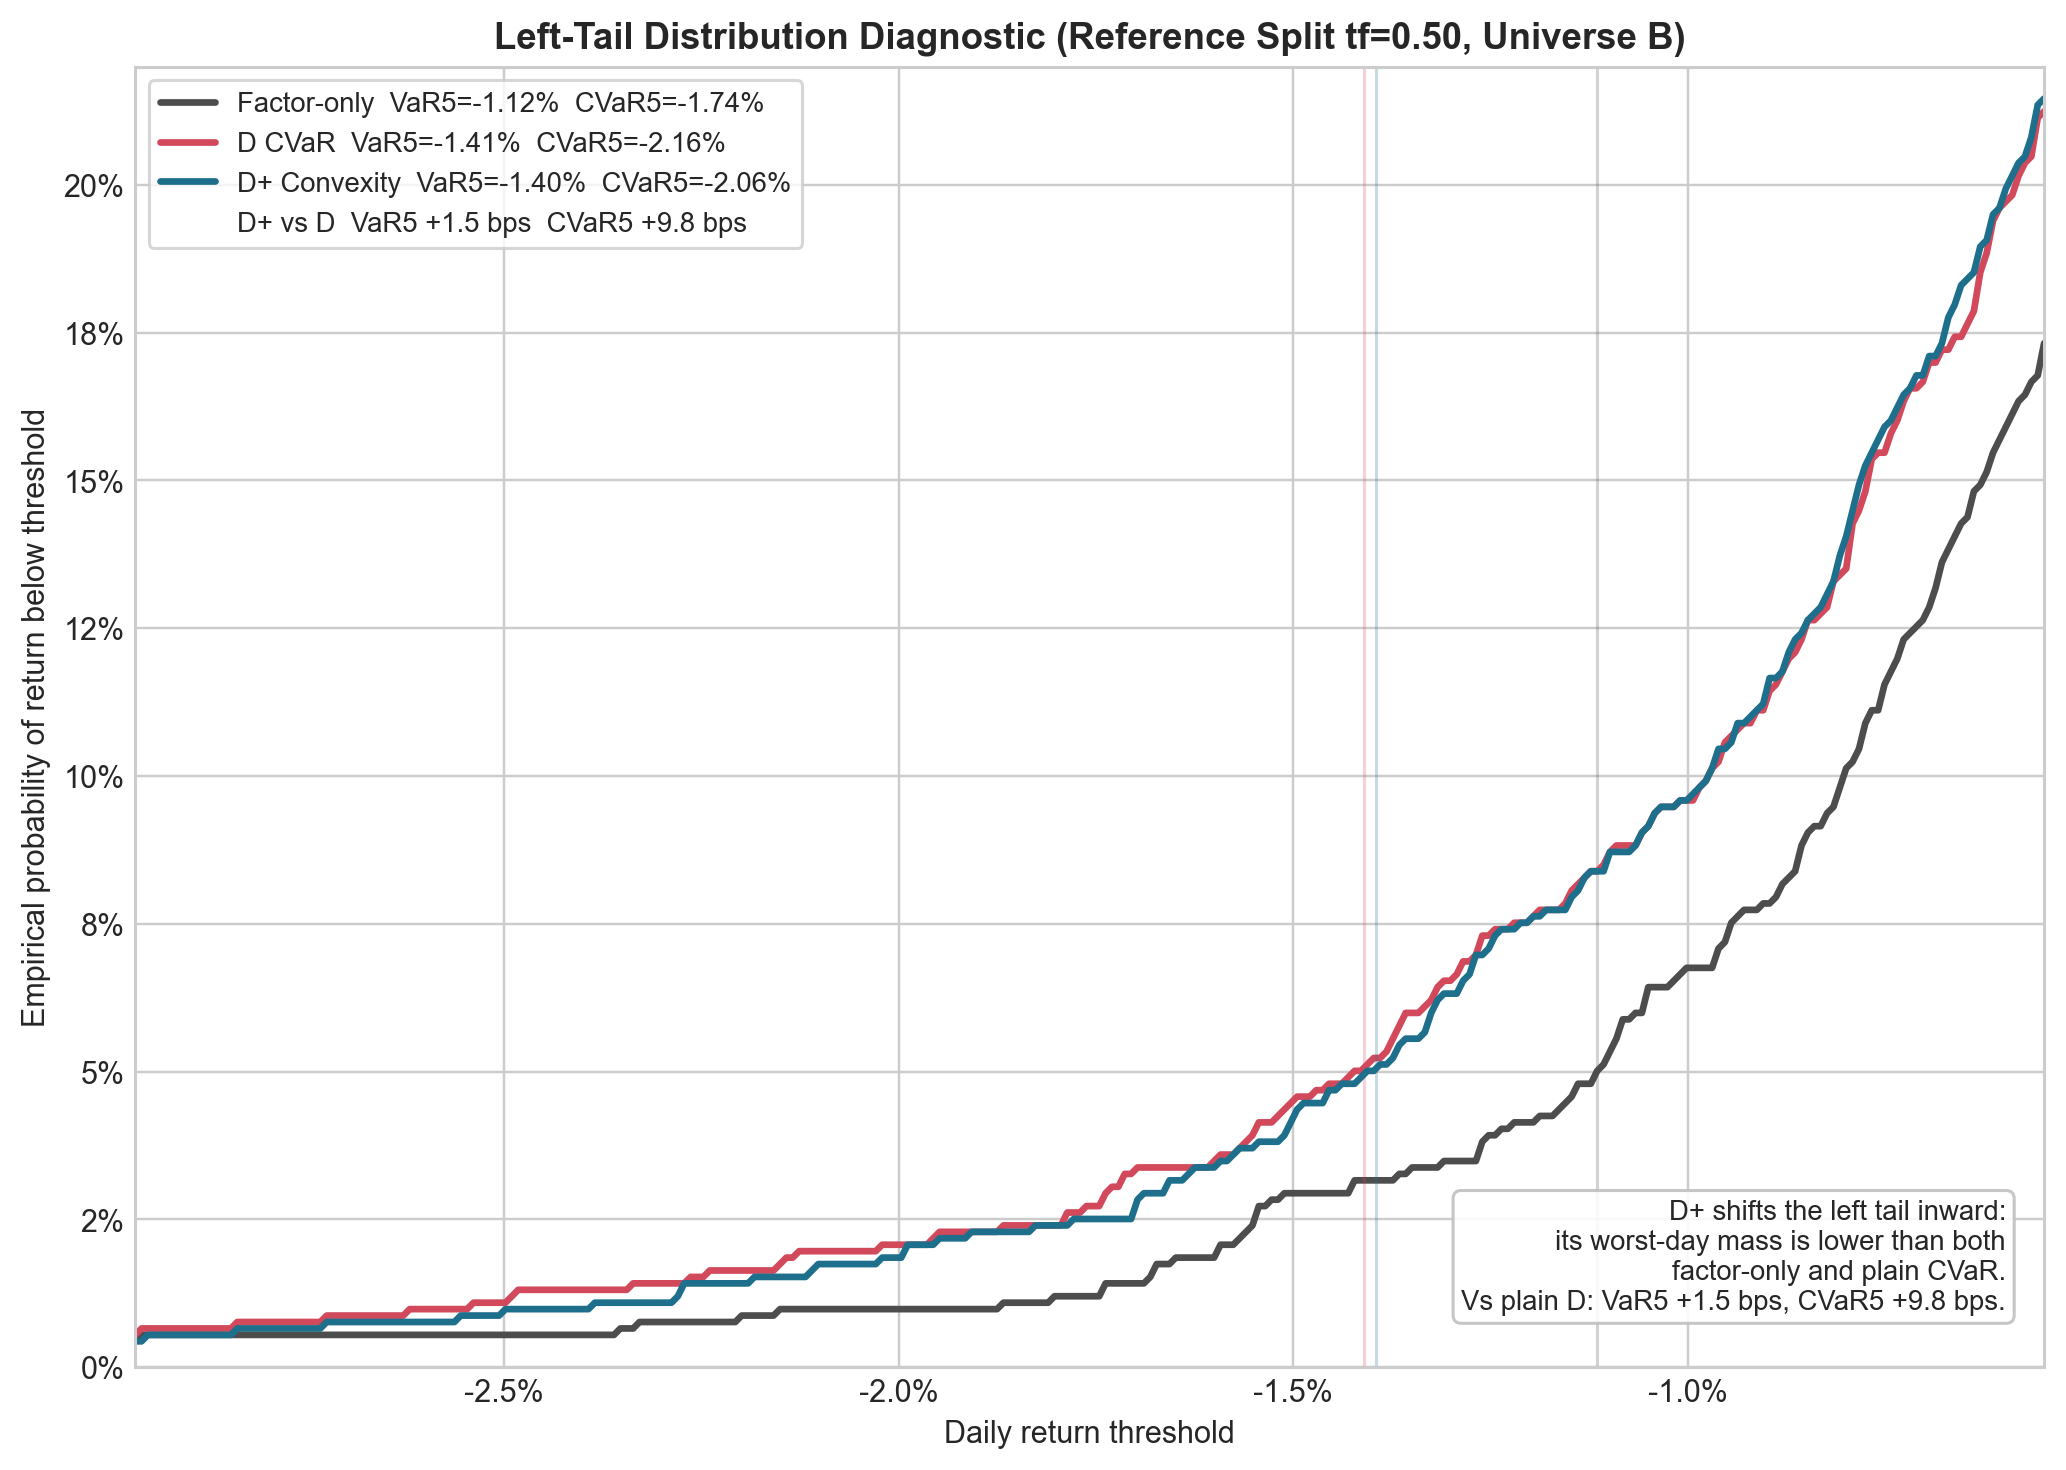
\includegraphics[width=0.95\linewidth]{../../results/20260331_002747_universe_B/control_tail_diagnostic.png}
\end{minipage}
\caption{Left-tail empirical distribution diagnostics for the reference split in
both universes. In Universe A, \texttt{D+} visibly improves the worst-return
mass relative to plain \texttt{D}; in Universe B, the tail improvement is
smaller, matching the tighter D-versus-D+ ranking in the tables.}
\label{fig:taildiagnostic}
\end{figure*}
}{}

\IfFileExists{../../results/20260330_221820_universe_A/control_mpc_diagnostic.png}{
\begin{figure*}[p]
\centering
\begin{minipage}{0.49\textwidth}
\centering
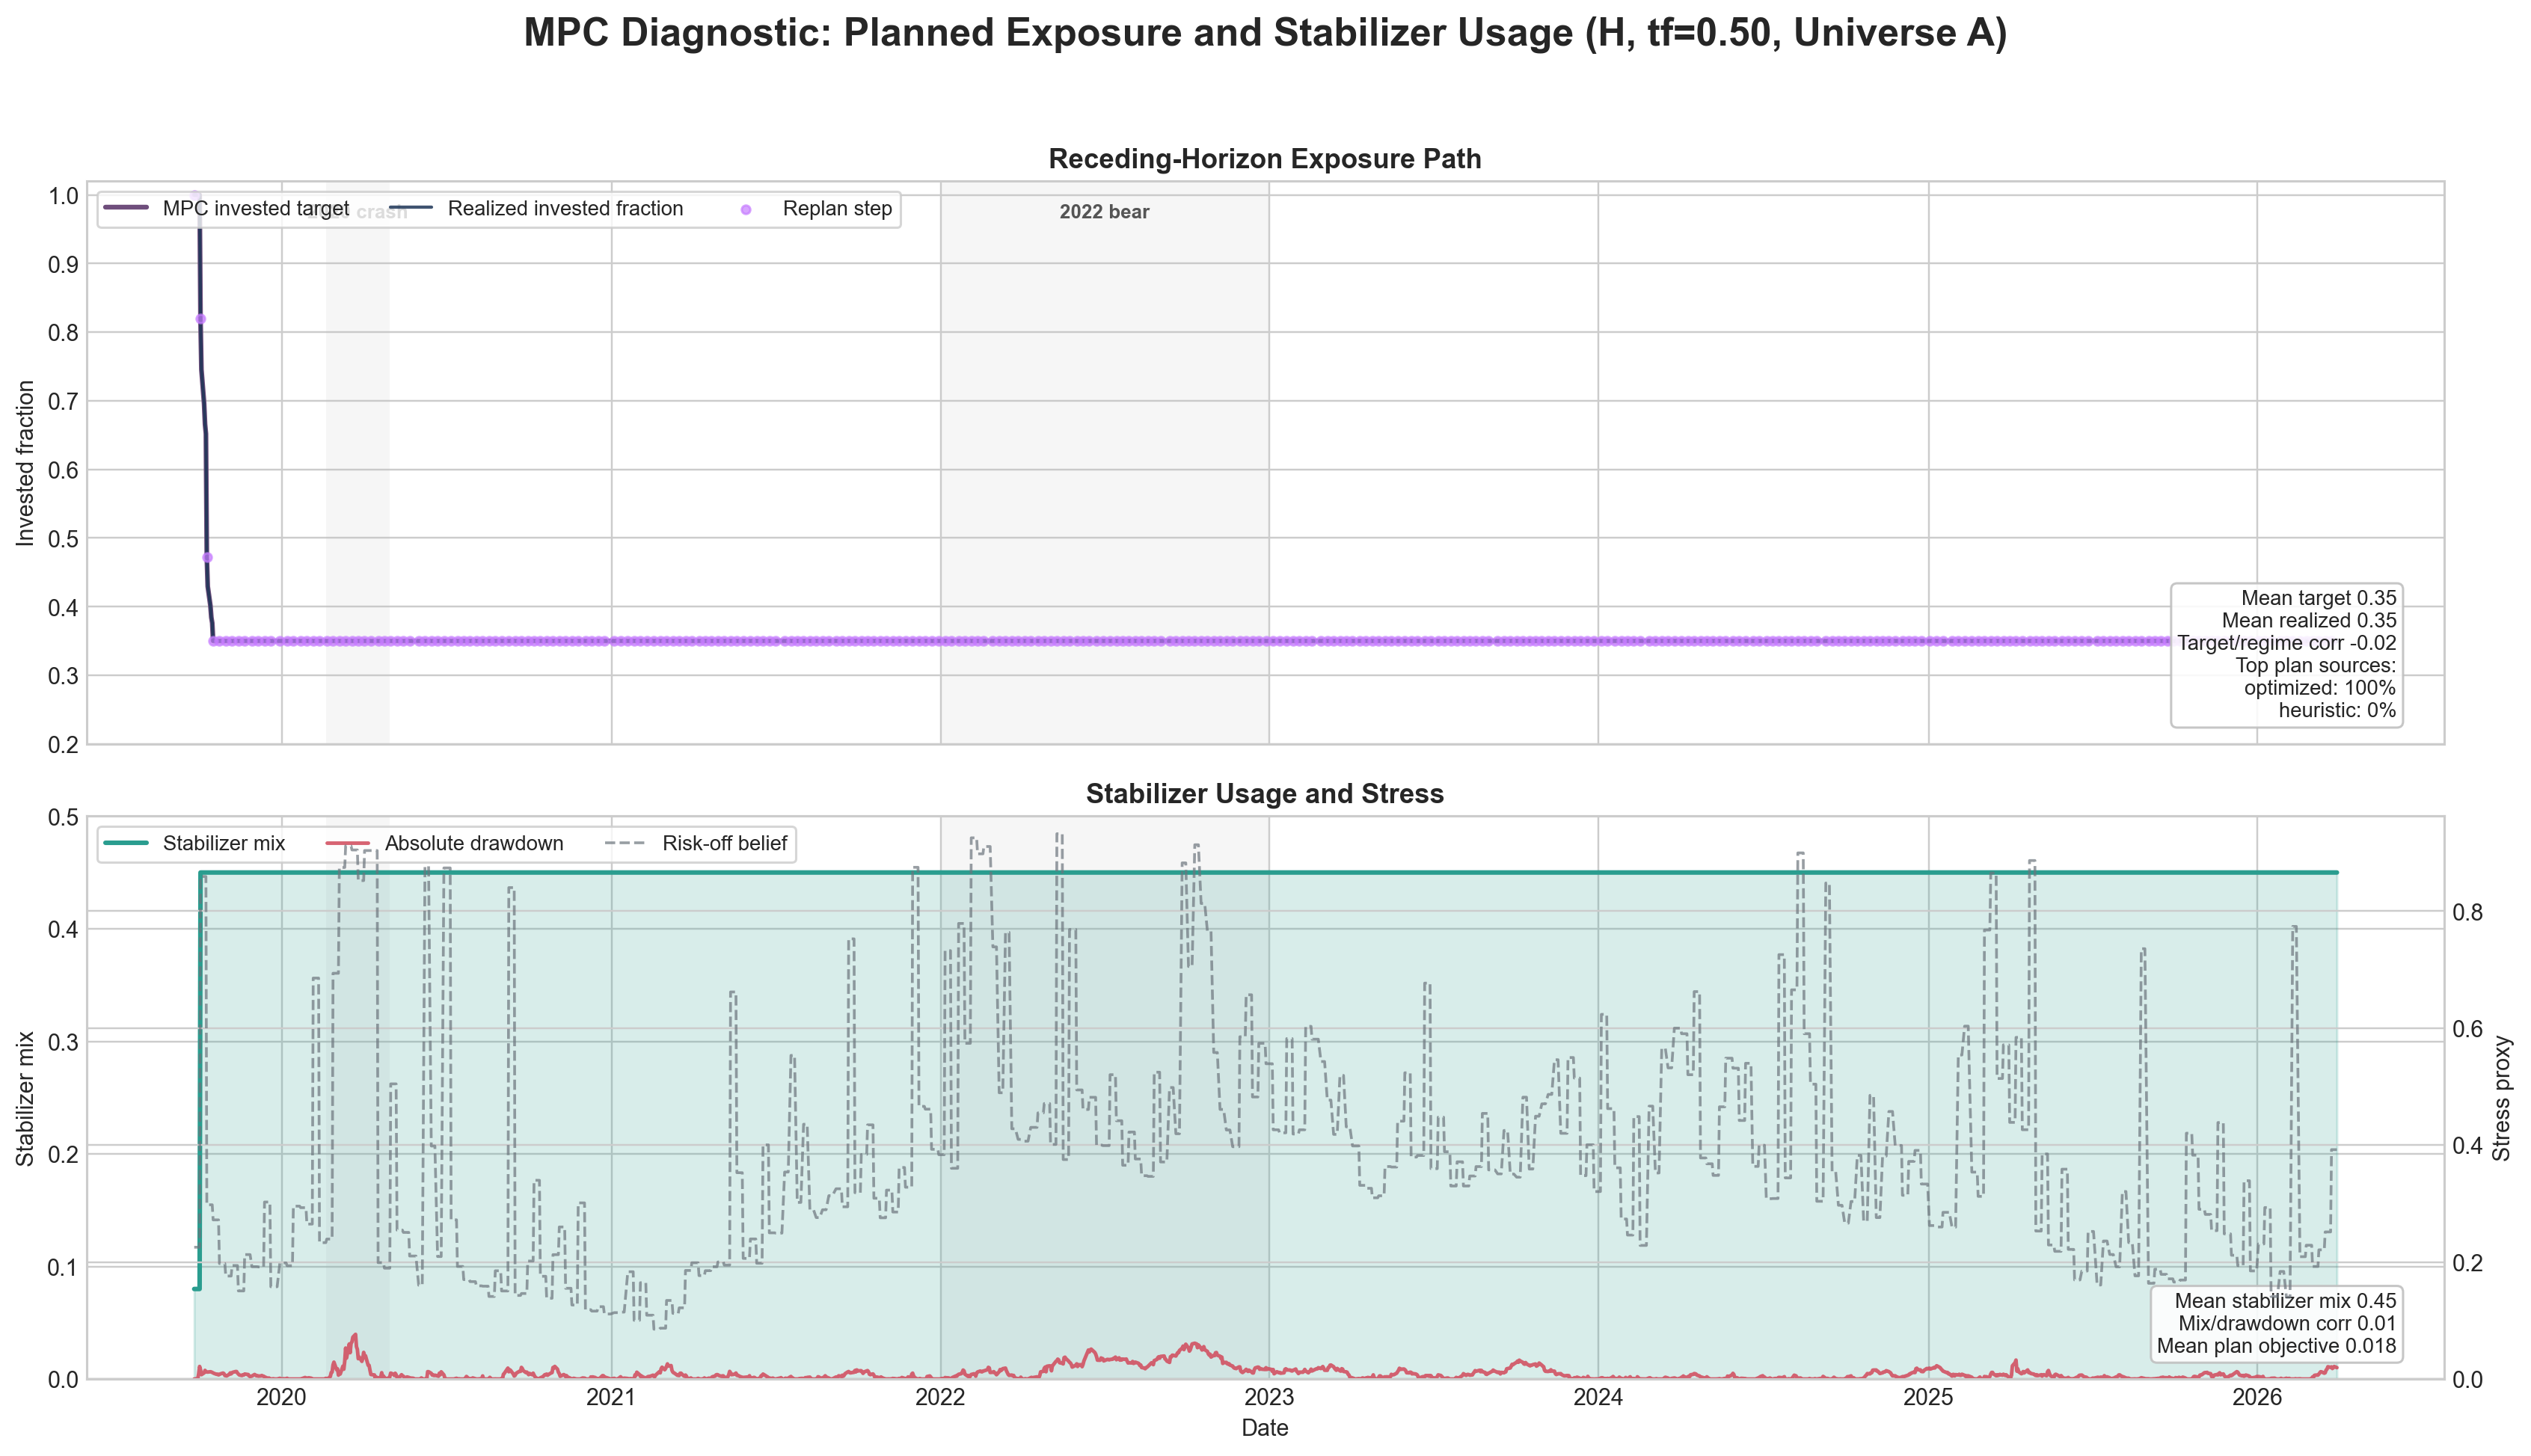
\includegraphics[width=\linewidth]{../../results/20260330_221820_universe_A/control_mpc_diagnostic.png}
\end{minipage}\hfill
\begin{minipage}{0.49\textwidth}
\centering
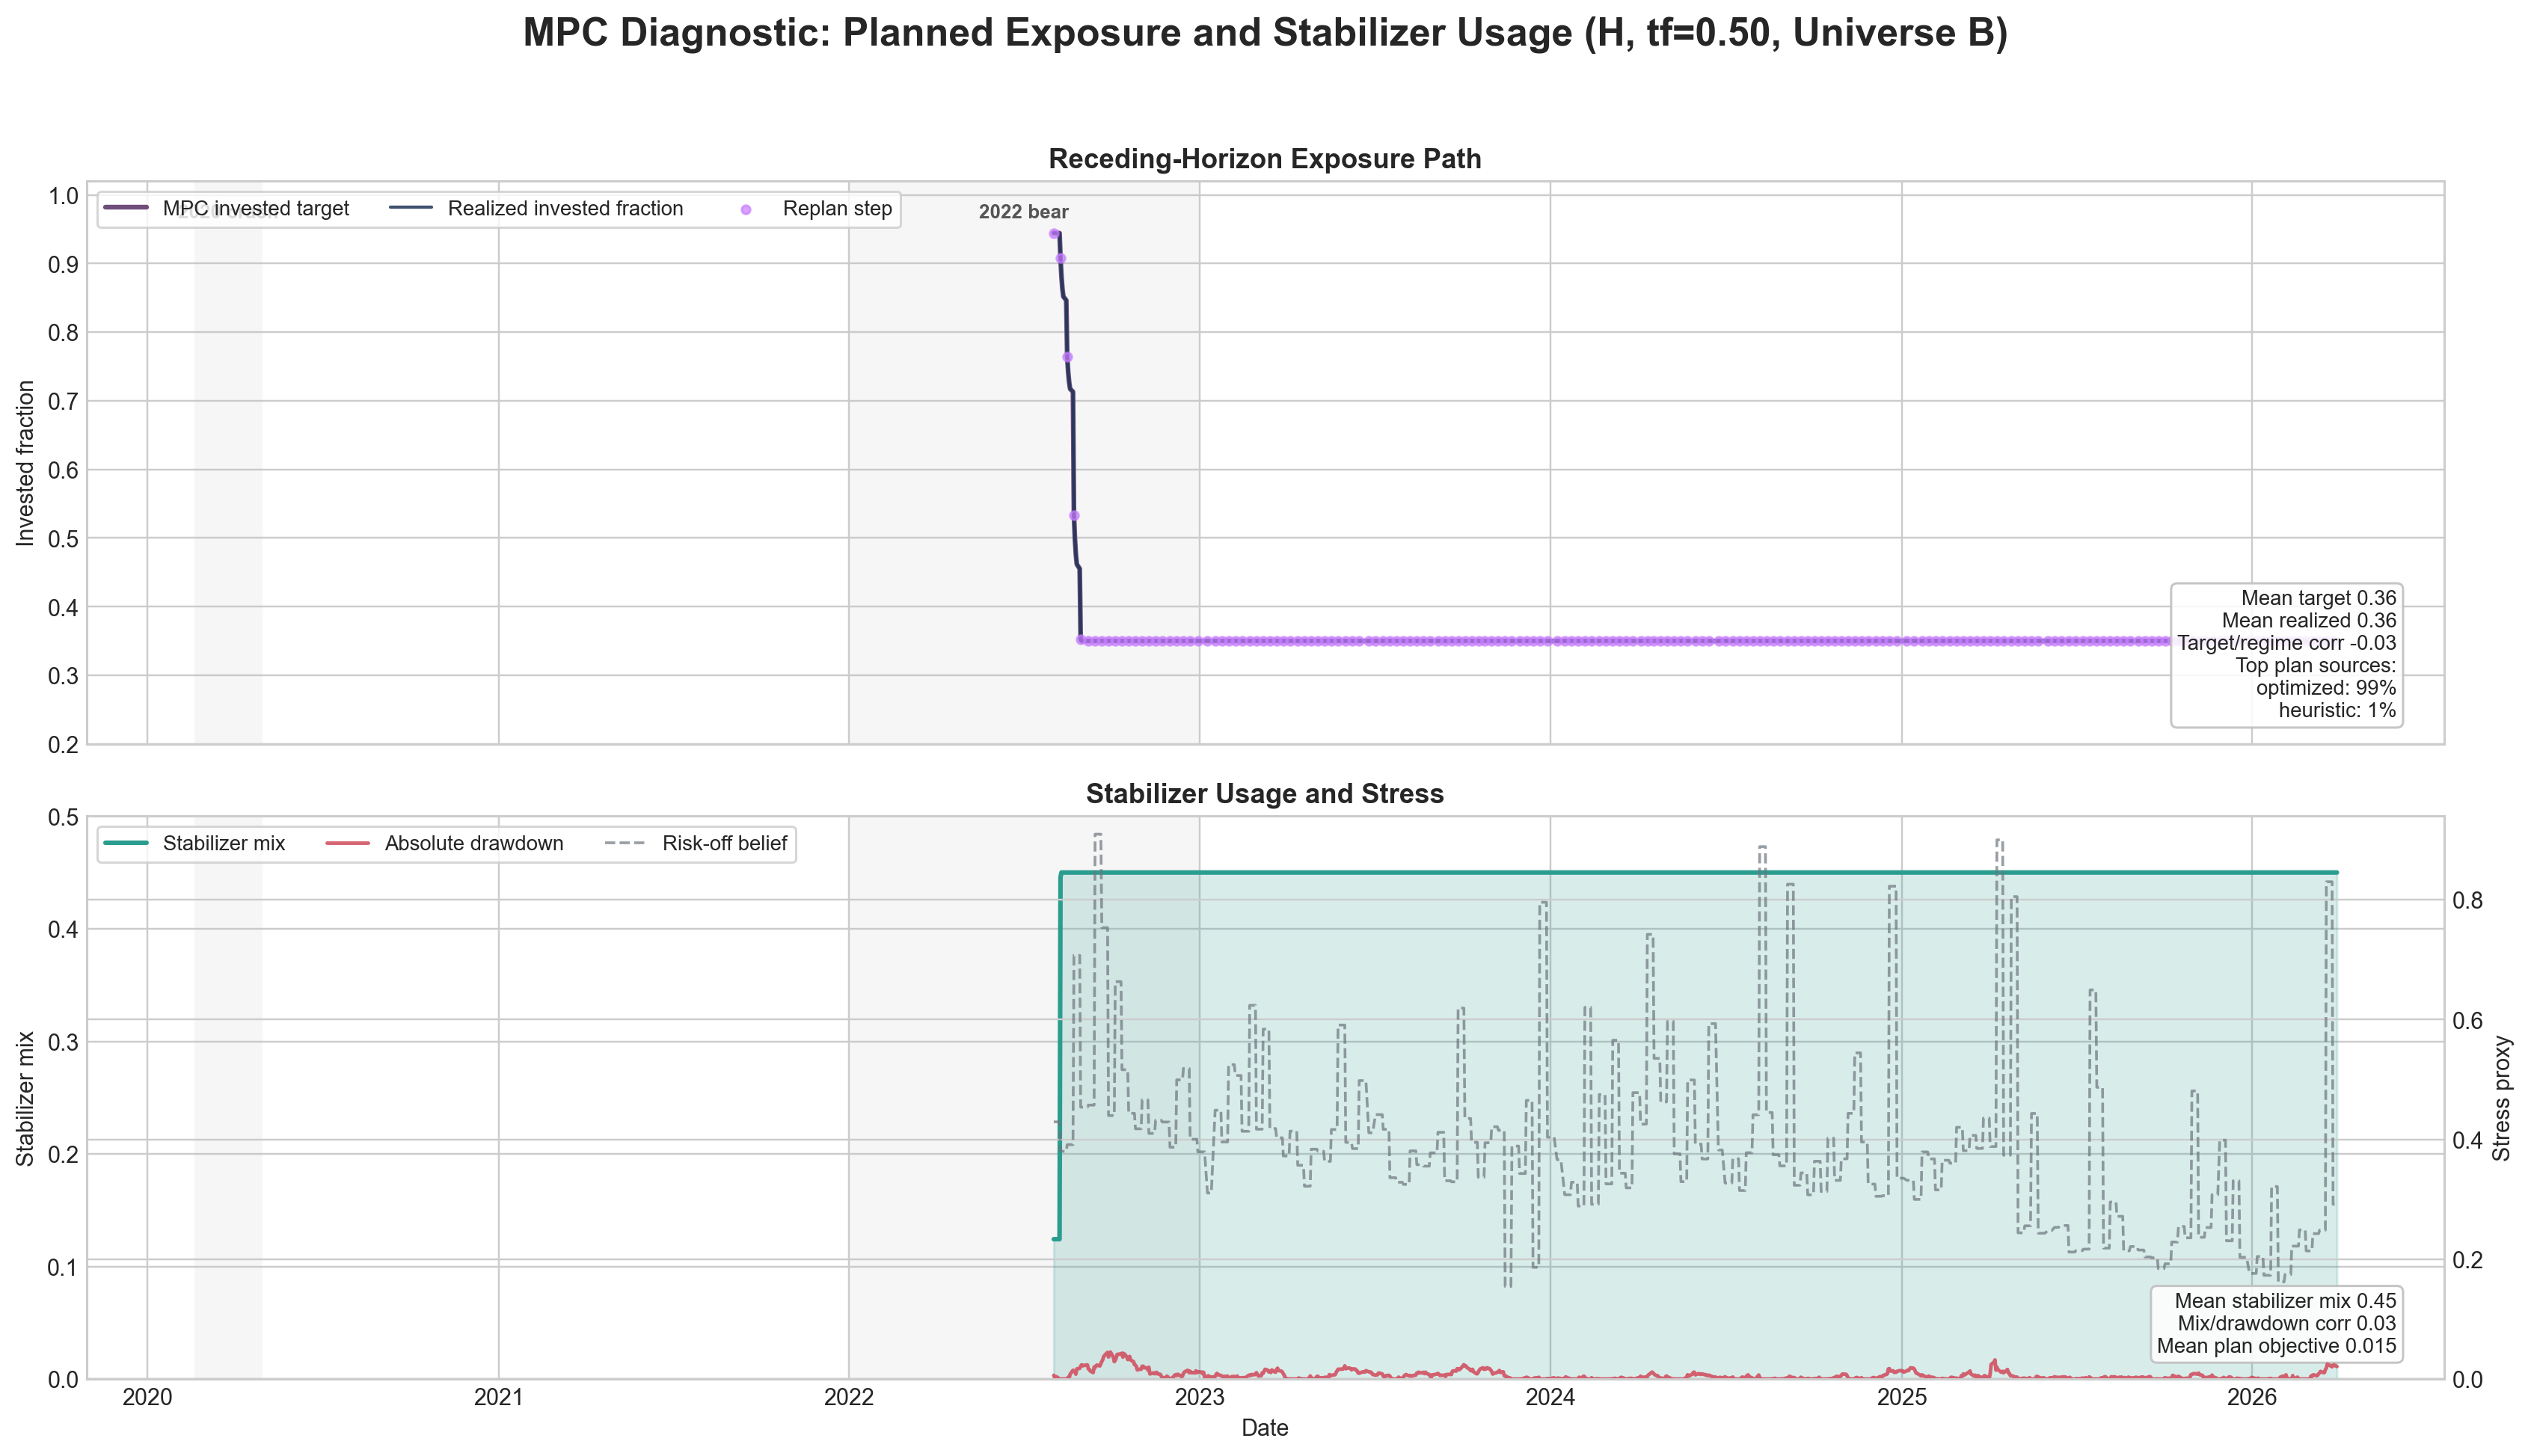
\includegraphics[width=\linewidth]{../../results/20260331_002747_universe_B/control_mpc_diagnostic.png}
\end{minipage}
\caption{MPC diagnostics for the reference split in both universes. The plots
show planned versus realized invested fraction, stabilizer mix, and stress
annotations, clarifying why \texttt{H\_mpc} sits on the low-drawdown frontier.}
\label{fig:mpcdiag}
\end{figure*}
}{}

\IfFileExists{../../results/20260330_221820_universe_A/legacy_pruning_story.png}{
\begin{figure*}[p]
\centering
\begin{minipage}{0.49\textwidth}
\centering
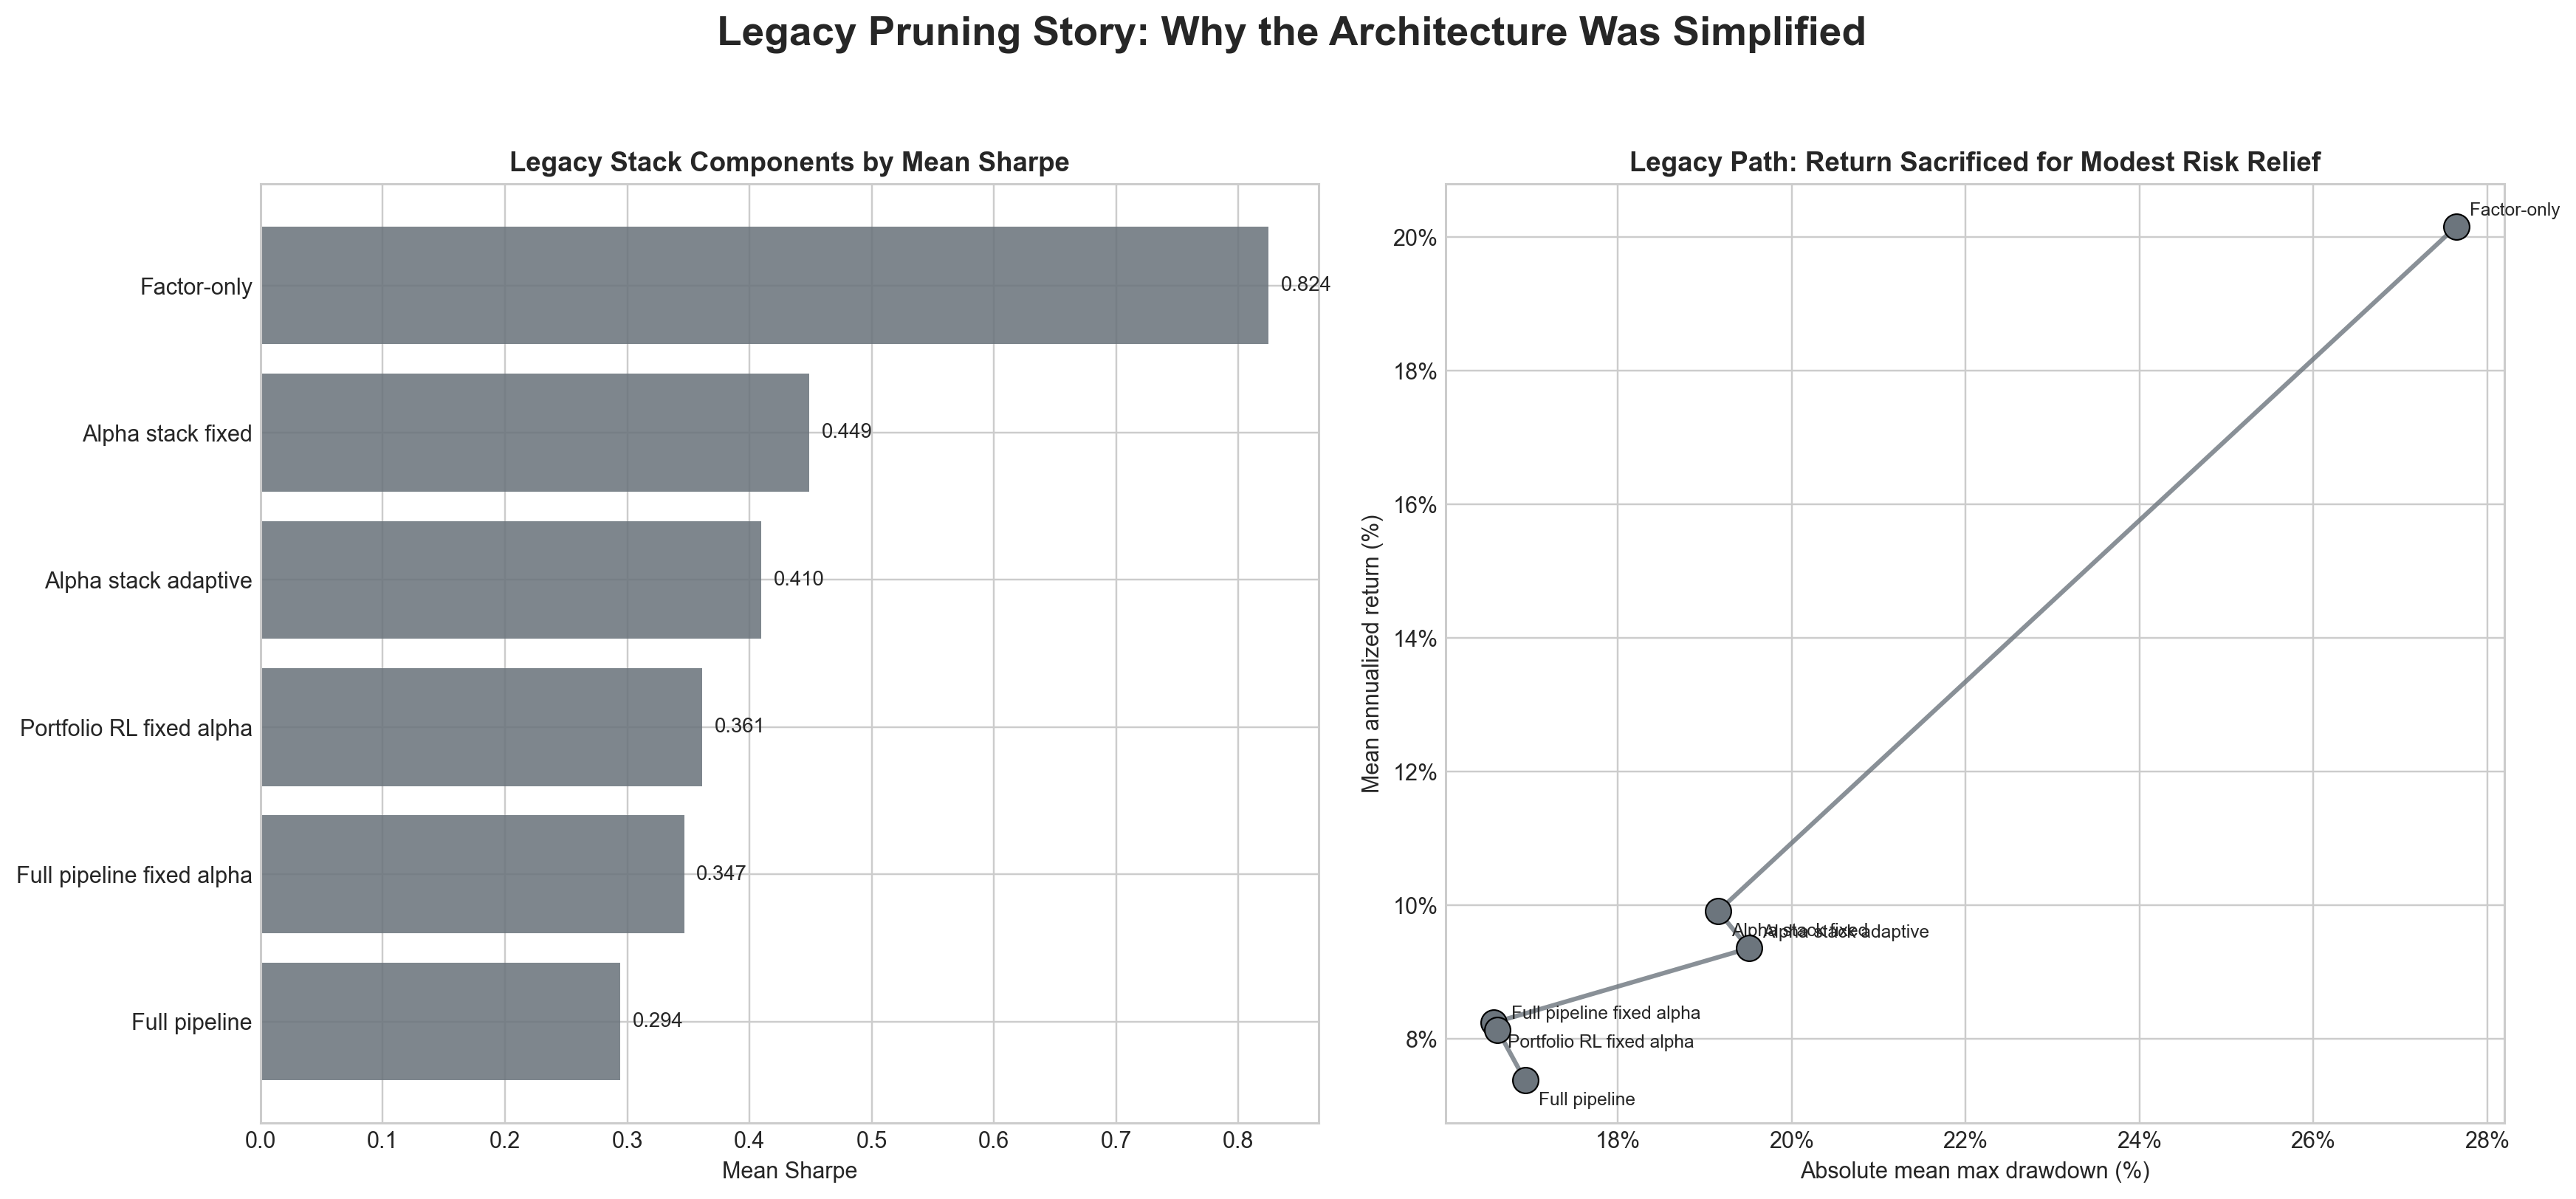
\includegraphics[width=\linewidth]{../../results/20260330_221820_universe_A/legacy_pruning_story.png}
\end{minipage}\hfill
\begin{minipage}{0.49\textwidth}
\centering
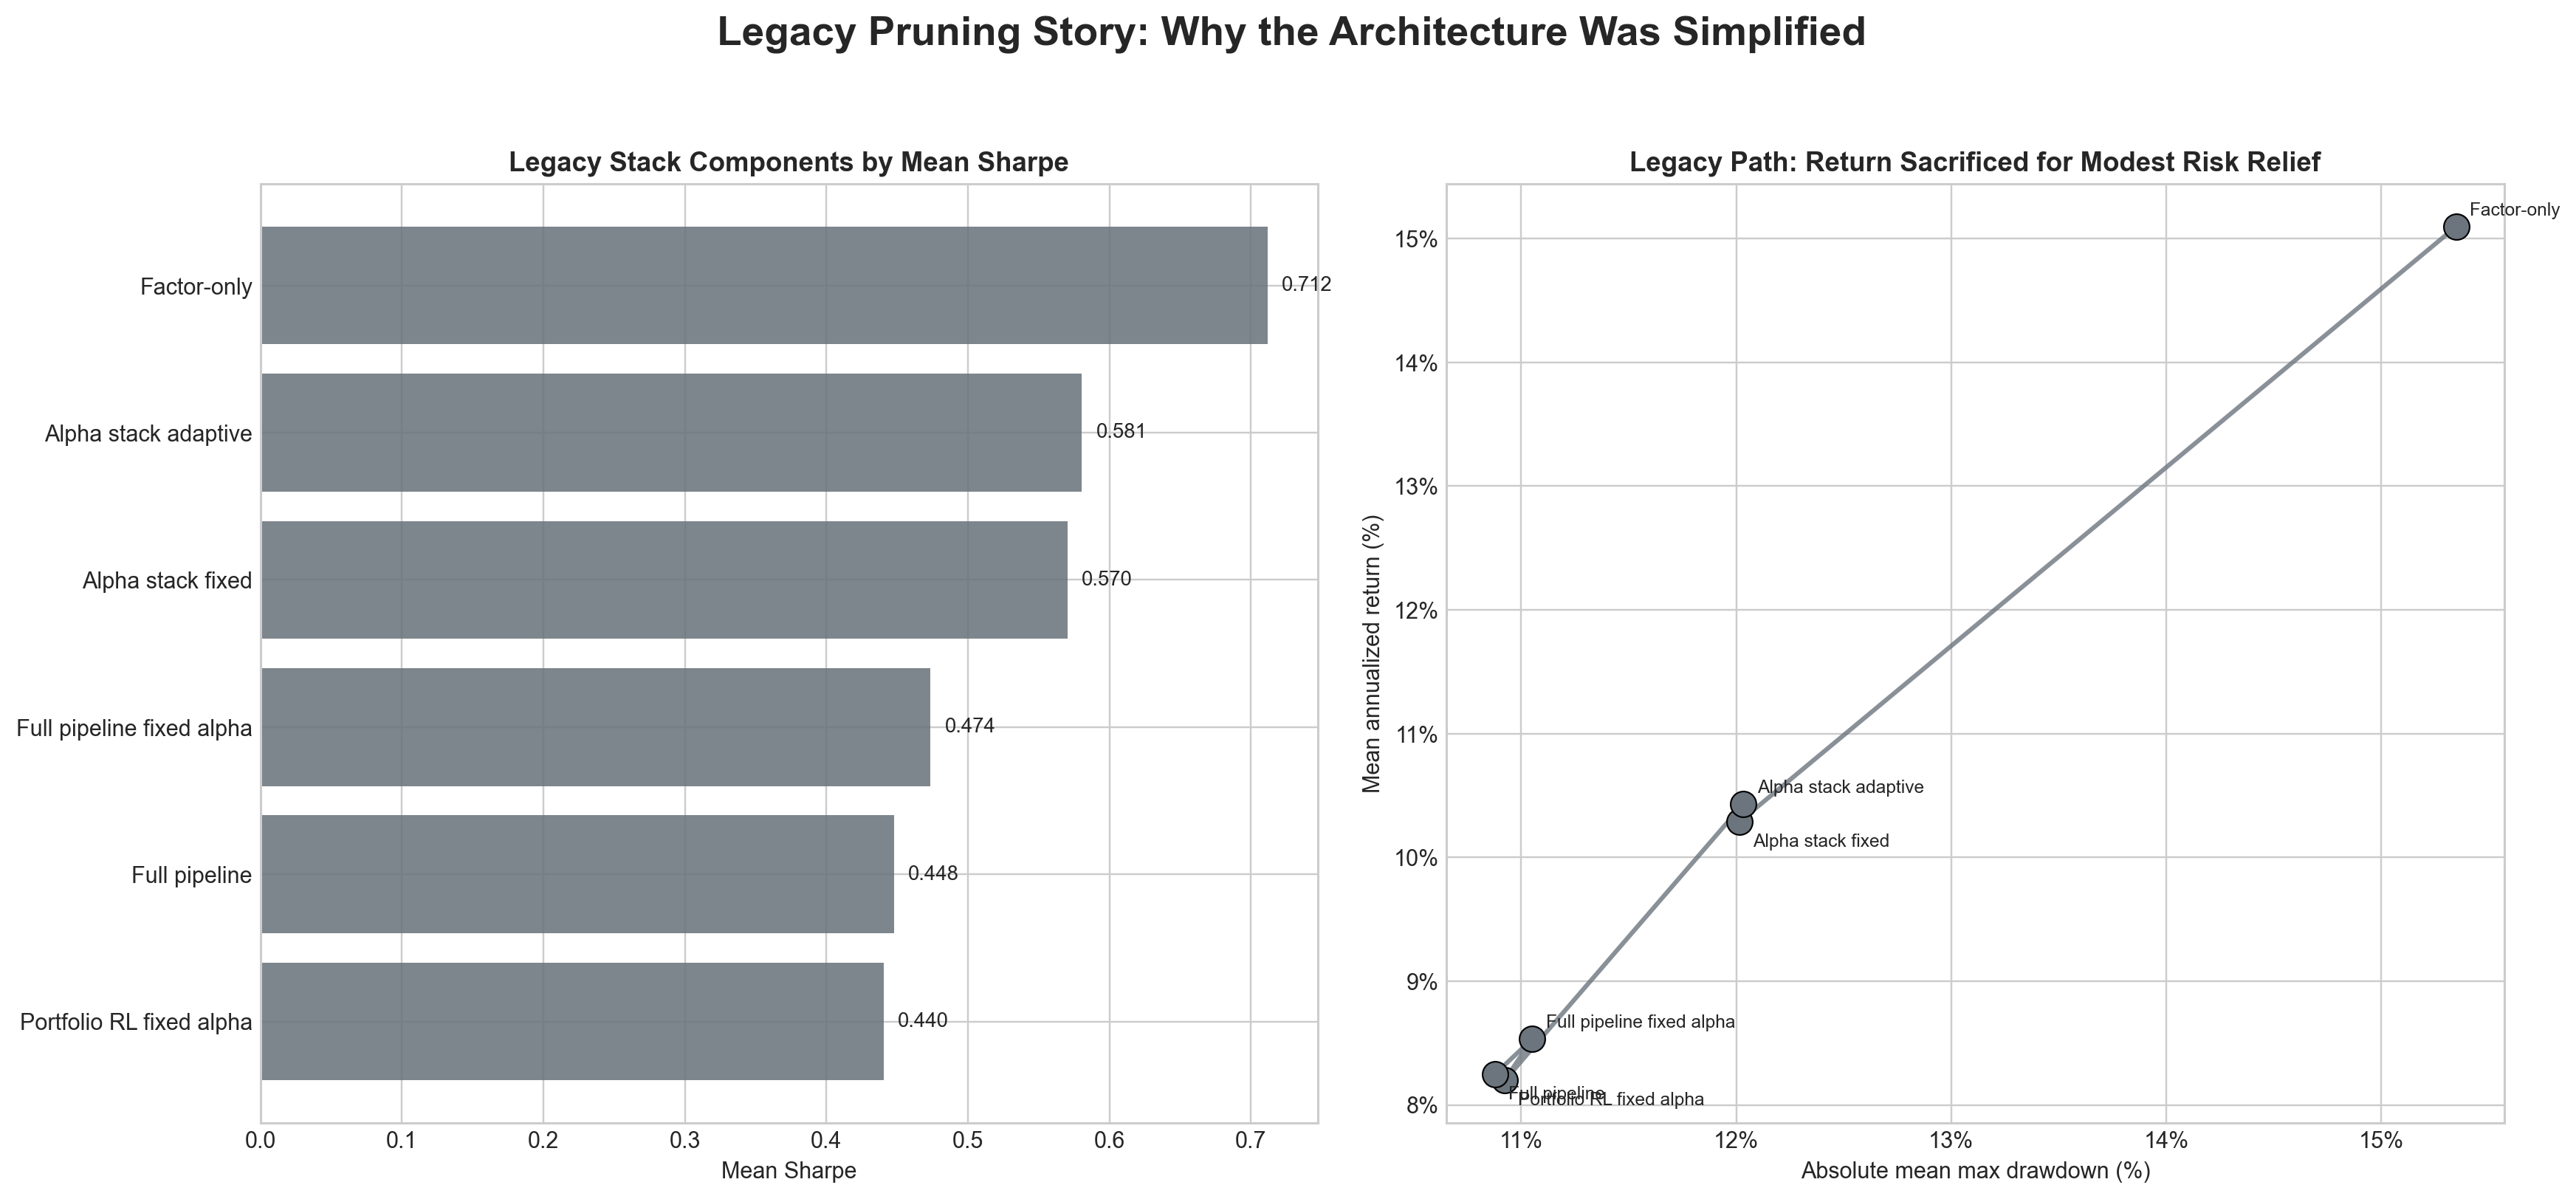
\includegraphics[width=\linewidth]{../../results/20260331_002747_universe_B/legacy_pruning_story.png}
\end{minipage}
\caption{Legacy pruning-story diagnostics for Universes A and B. These remain
useful as historical negative-reference evidence showing why the paper moved
away from the old RL-heavy stack.}
\label{fig:legacy_pruning}
\end{figure*}
}{}


\IfFileExists{../../results/20260330_221820_universe_A/pipeline_rolling_windows.png}{
\begin{figure*}[p]
\centering
\begin{minipage}{0.49\textwidth}
\centering
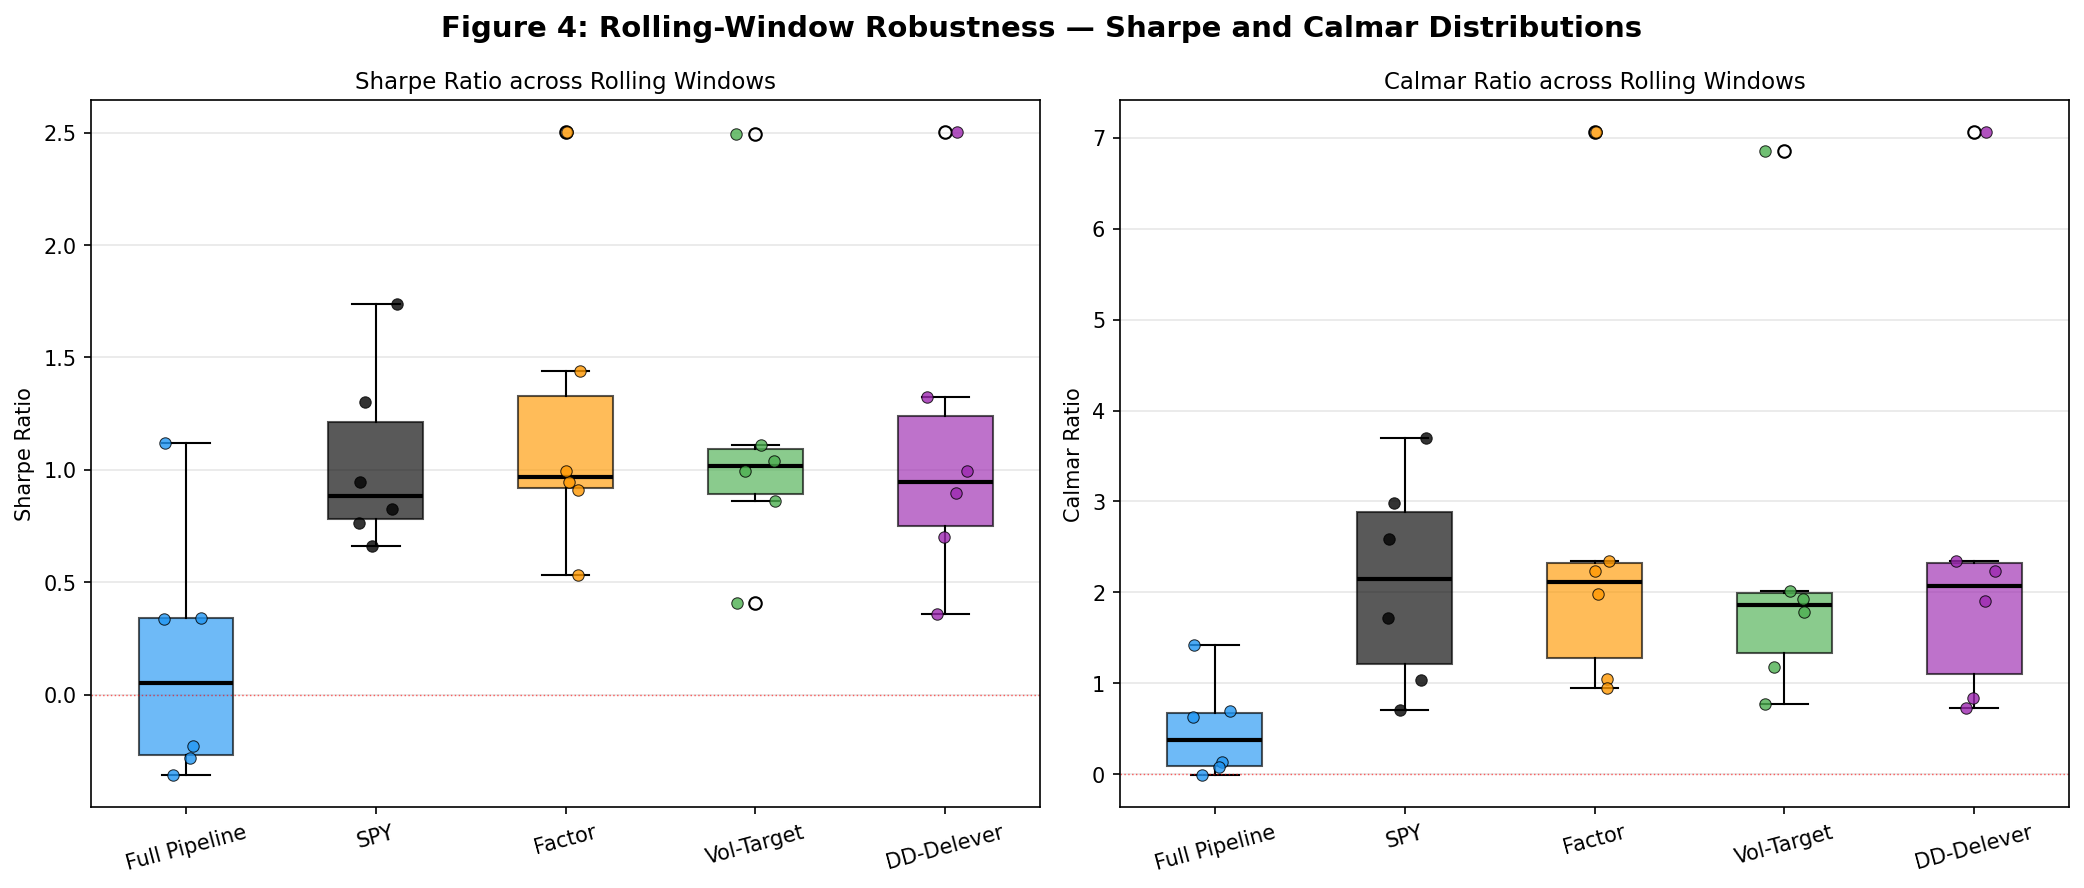
\includegraphics[width=\linewidth]{../../results/20260330_221820_universe_A/pipeline_rolling_windows.png}
\end{minipage}\hfill
\begin{minipage}{0.49\textwidth}
\centering
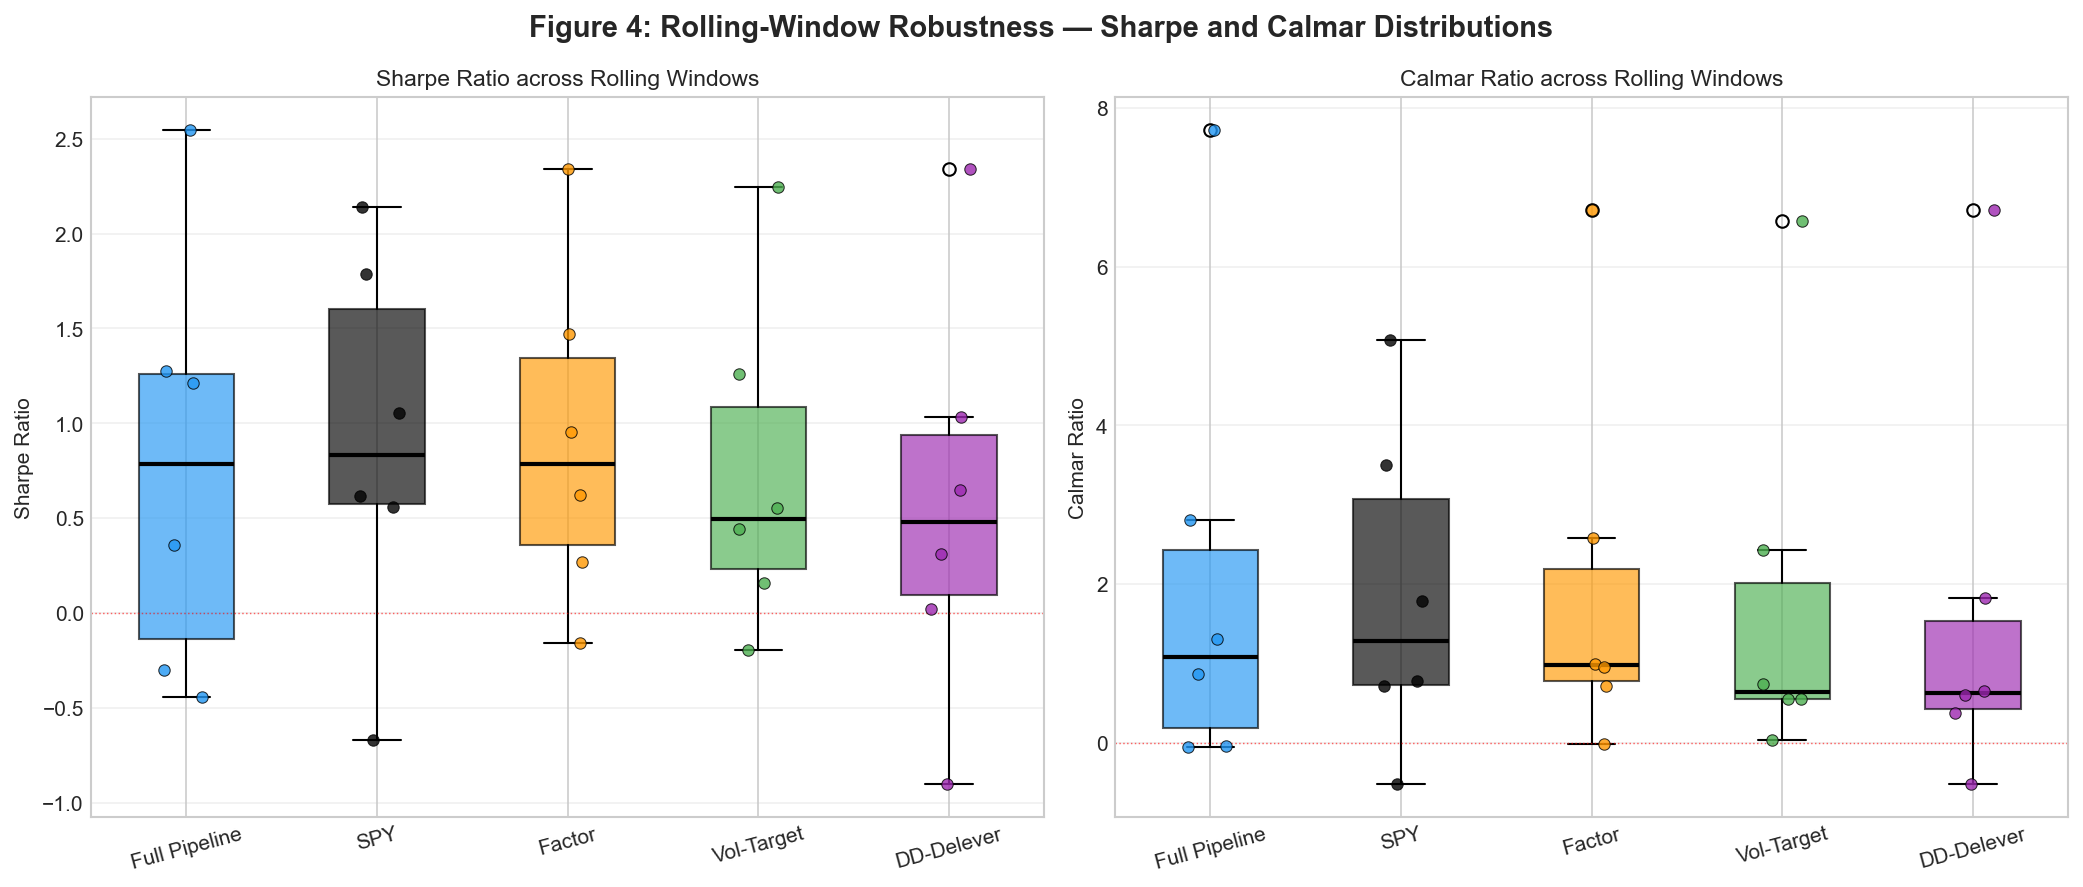
\includegraphics[width=\linewidth]{../../results/20260331_002747_universe_B/pipeline_rolling_windows.png}
\end{minipage}
\caption{Rolling-window robustness diagnostics for the retained legacy full
pipeline in both universes. The pattern remains mixed, and the windows should
be interpreted as internal robustness slices from one historical sample rather
than independent replications.}
\label{fig:rollingwindows}
\end{figure*}
}{}

\IfFileExists{../../results/20260330_221820_universe_A/pipeline_reward_ablation.png}{
\begin{figure*}[t]
\centering
\begin{minipage}{0.49\textwidth}
\centering
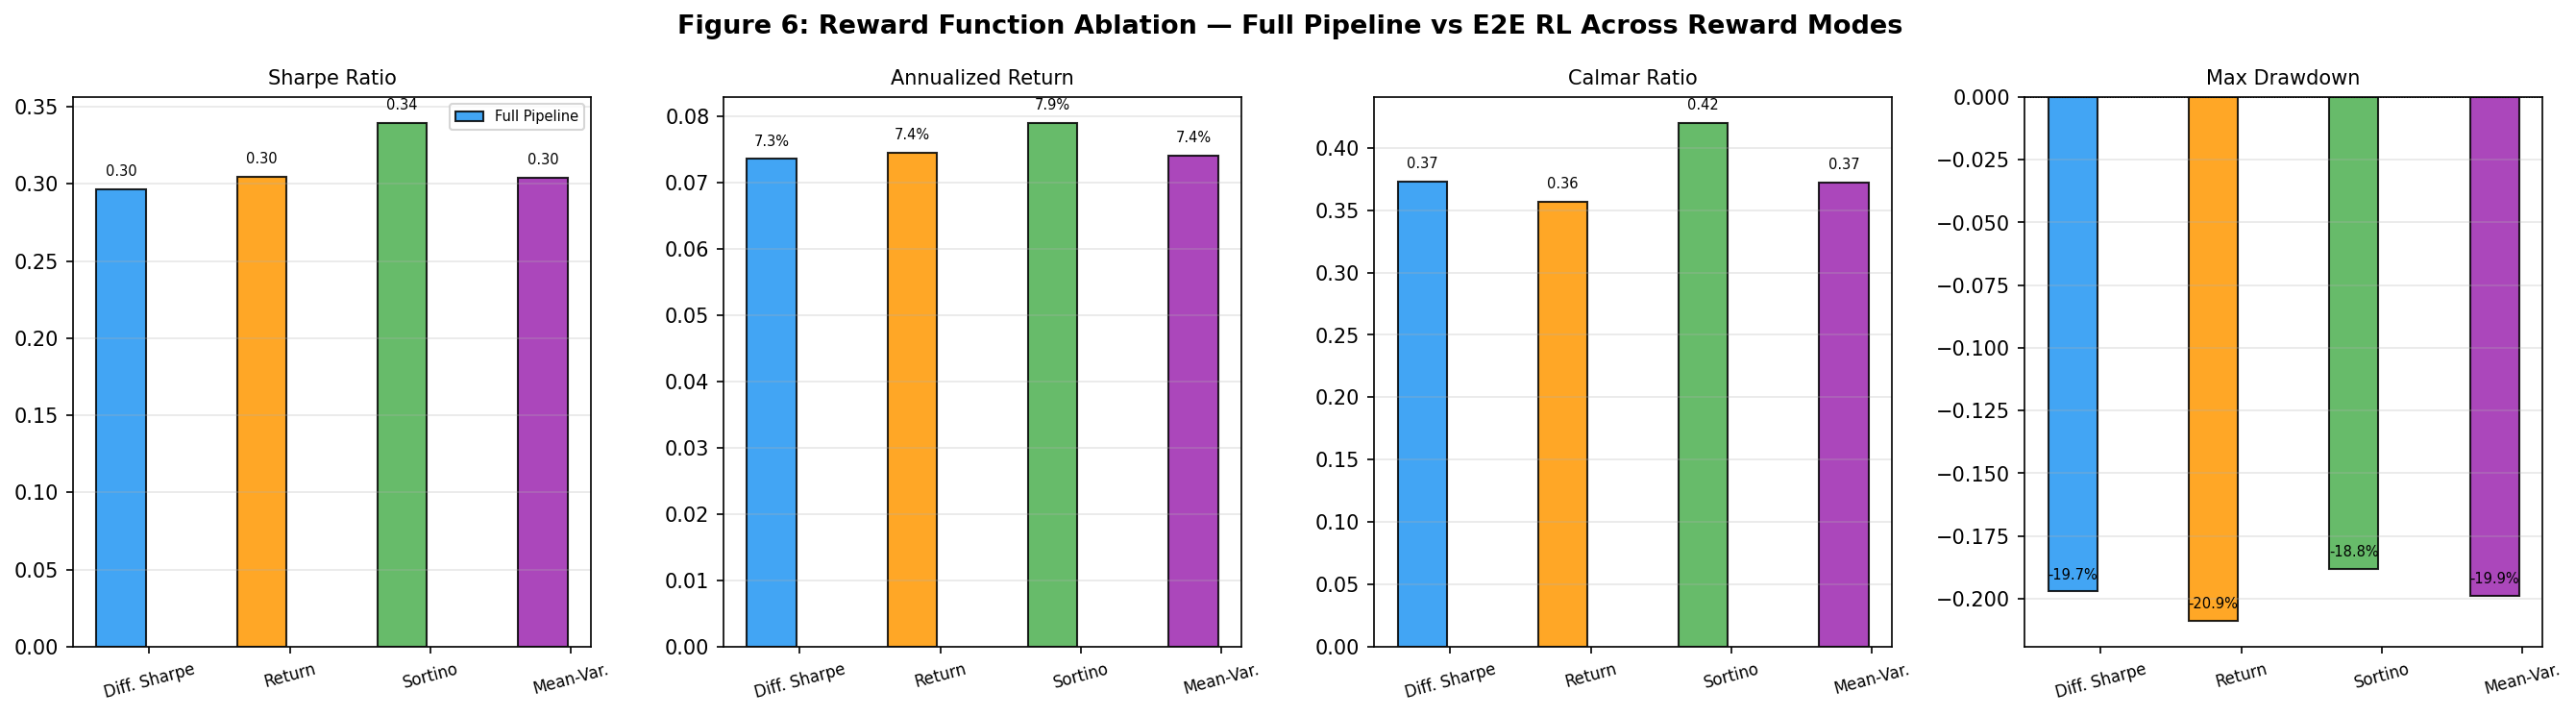
\includegraphics[width=\linewidth]{../../results/20260330_221820_universe_A/pipeline_reward_ablation.png}
\end{minipage}\hfill
\begin{minipage}{0.49\textwidth}
\centering
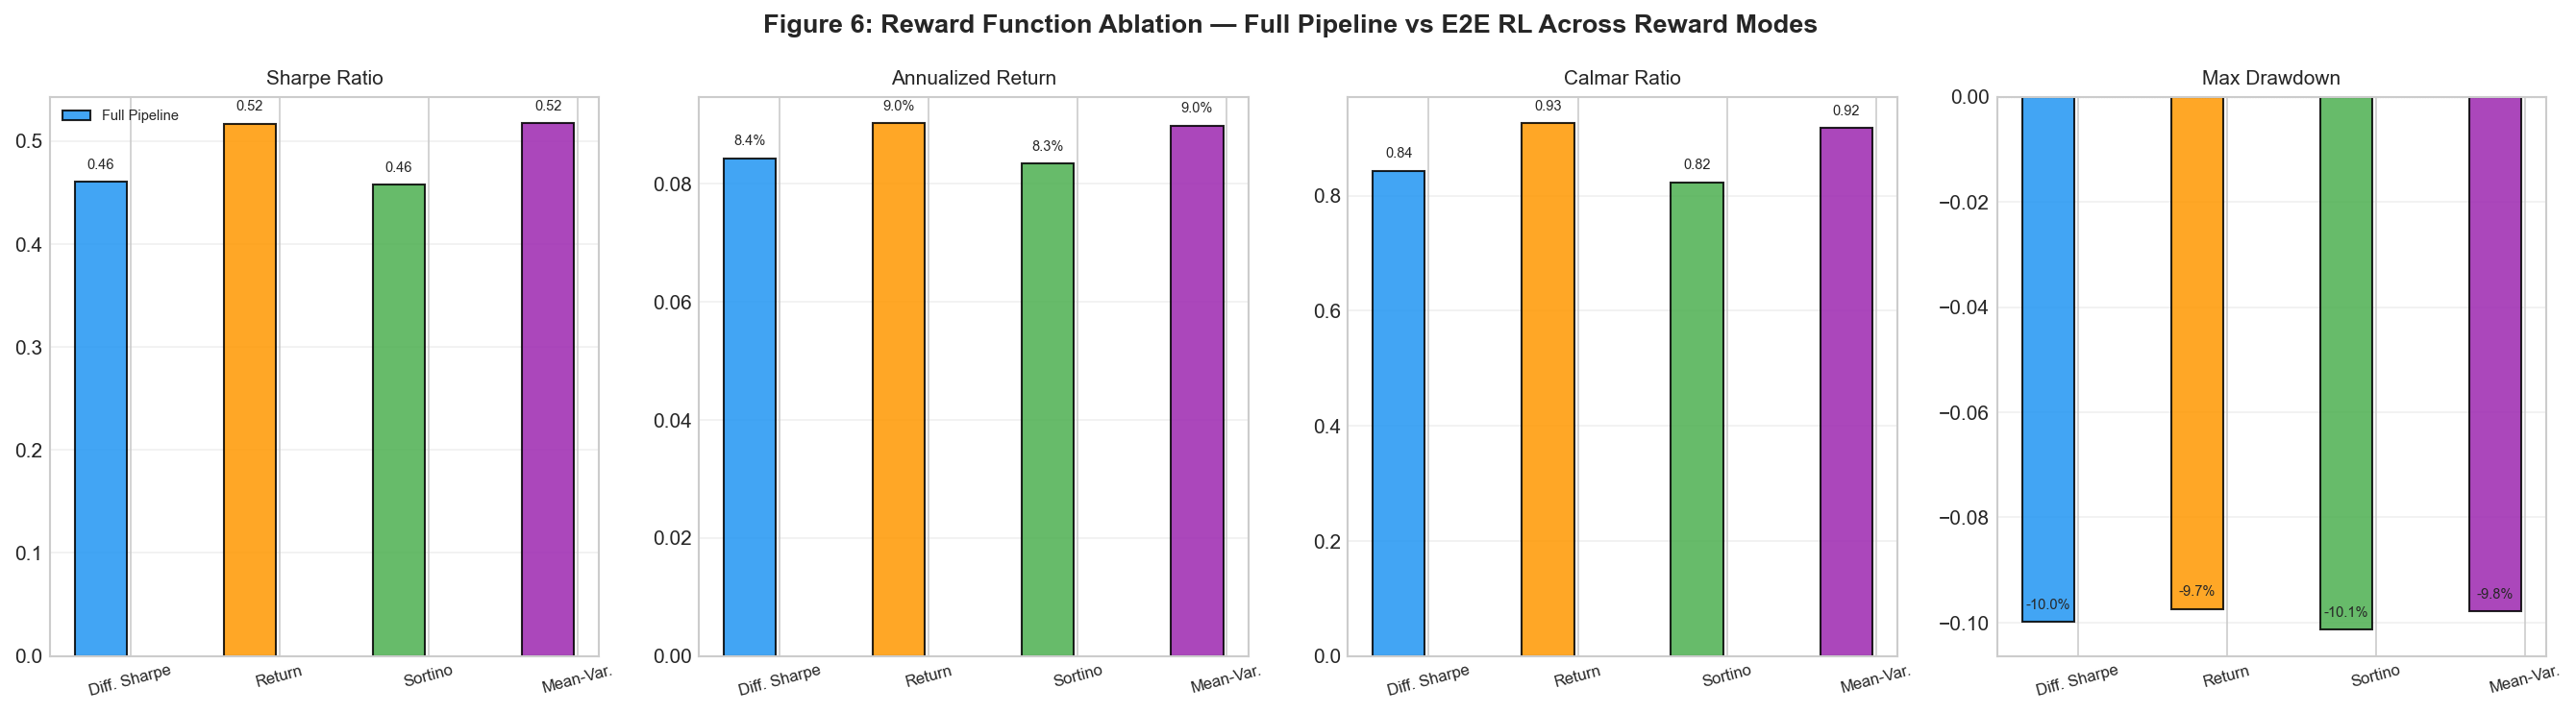
\includegraphics[width=\linewidth]{../../results/20260331_002747_universe_B/pipeline_reward_ablation.png}
\end{minipage}
\caption{Reward-ablation figures for the revised bundle in both universes.
Reward choice moves the legacy controller within a narrow band, but does not
change the broader ranking versus the factor core and the strongest robust
controllers.}
\label{fig:rewardfig}
\end{figure*}
}{}

\clearpage
\begin{thebibliography}{99}

\bibitem{agrawal2013} % *** NEW ***
S. Agrawal and N. Goyal.
\newblock Thompson sampling for contextual bandits with linear payoffs.
\newblock In \emph{International Conference on Machine Learning}, pages 127--135, 2013.

% ============================================================================
% MEAN-CVAR OPTIMIZATION (NEW)
% ============================================================================

\bibitem{alexander2006} % *** NEW ***
S. Alexander, T. F. Coleman, and Y. Li.
\newblock Minimizing CVaR and VaR for a portfolio of derivatives.
\newblock \emph{Journal of Banking \& Finance}, 30(2):583--605, 2006.

% ============================================================================
% EXECUTION & TRANSACTION COSTS
% ============================================================================

\bibitem{almgren2000}
R. Almgren and N. Chriss.
\newblock Optimal execution of portfolio transactions.
\newblock \emph{Journal of Risk}, 3(2):5--39, 2000.

% ============================================================================
% CONSTRAINED MDPS (NEW - FOR YOUR CMDP CONTROLLER)
% ============================================================================

\bibitem{altman1999} % *** NEW ***
E. Altman.
\newblock \emph{Constrained Markov Decision Processes}.
\newblock CRC Press, 1999.

% ============================================================================
% COHERENT RISK MEASURES (NEW - CRITICAL FOR CVAR)
% ============================================================================

\bibitem{artzner1999} % *** NEW ***
P. Artzner, F. Delbaen, J.-M. Eber, and D. Heath.
\newblock Coherent measures of risk.
\newblock \emph{Mathematical Finance}, 9(3):203--228, 1999.

% ============================================================================
% VOLATILITY MODELS
% ============================================================================

\bibitem{bollerslev1986}
T. Bollerslev.
\newblock Generalized autoregressive conditional heteroskedasticity.
\newblock \emph{Journal of Econometrics}, 31(3):307--327, 1986.

% ============================================================================
% CONSTRAINED MDPS - LAGRANGIAN (NEW - FOR YOUR CMDP CONTROLLER)
% ============================================================================

\bibitem{borkar2005} % *** NEW ***
V. S. Borkar.
\newblock An actor-critic algorithm for constrained Markov decision processes.
\newblock \emph{Systems \& Control Letters}, 54(3):207--213, 2005.

% ============================================================================
% RL FOR HEDGING
% ============================================================================

\bibitem{buehler2019}
H. Buehler, L. Gonon, J. Teichmann, and B. Wood.
\newblock Deep hedging.
\newblock \emph{Quantitative Finance}, 19(8):1271--1291, 2019.

% ============================================================================
% MODEL PREDICTIVE CONTROL (NEW - FOR YOUR MPC CONTROLLER)
% ============================================================================

\bibitem{camacho2013} % *** NEW ***
E. F. Camacho and C. B. Alba.
\newblock \emph{Model Predictive Control}.
\newblock Springer Science \& Business Media, 2013.

% ============================================================================
% MACHINE LEARNING IN ASSET PRICING
% ============================================================================

\bibitem{chen2021}
L. Chen, M. Pelger, and J. Zhu.
\newblock Deep learning in asset pricing.
\newblock \emph{SSRN Working Paper 3350138}, revised 2021.

% ============================================================================
% RL FOR PORTFOLIO MANAGEMENT
% ============================================================================

\bibitem{cong2021}
Y. Cong, B. Deng, X. Bao, and H. Dai.
\newblock AlphaPortfolio: Direct construction through deep reinforcement learning
  and interpretable representation learning.
\newblock \emph{Proceedings of the AAAI Conference on Artificial Intelligence},
  35(6):4831--4839, 2021.

% ============================================================================
% DISTRIBUTIONALLY ROBUST OPTIMIZATION (NEW)
% ============================================================================

\bibitem{delage2010} % *** NEW ***
E. Delage and Y. Ye.
\newblock Distributionally robust optimization under moment uncertainty with application to data-driven problems.
\newblock \emph{Operations Research}, 58(3):595--612, 2010.

% ============================================================================
% RL FOR TRADING
% ============================================================================

\bibitem{deng2017}
Y. Deng, F. Bao, Y. Kong, Z. Ren, and Q. Dai.
\newblock Deep direct reinforcement learning for financial signal representation
  and trading.
\newblock \emph{IEEE Transactions on Neural Networks and Learning Systems},
  28(3):653--664, 2017.

% ============================================================================
% RL FOR HEDGING
% ============================================================================

\bibitem{du2020}
Y. Du, P. N. Kolm, A. Ritter, and T. Wang.
\newblock Deep reinforcement learning for option replication and hedging.
\newblock \emph{The Journal of Financial Data Science}, 2(4):44--59, 2020.

% ============================================================================
% VOLATILITY MODELS
% ============================================================================

\bibitem{engle1982}
R. F. Engle.
\newblock Autoregressive conditional heteroscedasticity with estimates of the
  variance of United Kingdom inflation.
\newblock \emph{Econometrica}, 50(4):987--1007, 1982.

% ============================================================================
% ROBUST PORTFOLIOS (NEW)
% ============================================================================

\bibitem{fabozzi2010} % *** NEW ***
F. J. Fabozzi, D. Huang, and G. Zhou.
\newblock Robust portfolios: contributions from operations research and finance.
\newblock \emph{Annals of Operations Research}, 176(1):191--220, 2010.

% ============================================================================
% FACTOR INVESTING
% ============================================================================

\bibitem{fama1993}
E. F. Fama and K. R. French.
\newblock Common risk factors in the returns on stocks and bonds.
\newblock \emph{Journal of Financial Economics}, 33(1):3--56, 1993.

% ============================================================================
% MACHINE LEARNING IN ASSET PRICING
% ============================================================================

\bibitem{giglio2022}
S. Giglio, D. Xiu, and D. Zhang.
\newblock Machine learning in asset pricing.
\newblock \emph{Annual Review of Financial Economics}, 14:337--368, 2022.

\bibitem{gu2020}
S. Gu, B. Kelly, and D. Xiu.
\newblock Empirical asset pricing via machine learning.
\newblock \emph{Review of Financial Studies}, 33(5):2223--2273, 2020.

% ============================================================================
% REGIME SWITCHING
% ============================================================================

\bibitem{hamilton1989}
J. D. Hamilton.
\newblock A new approach to the economic analysis of nonstationary time series
  and the business cycle.
\newblock \emph{Econometrica}, 57(2):357--384, 1989.

% ============================================================================
% META-LEARNING (NEW - FOR YOUR COUNCIL/MLP CONTROLLERS)
% ============================================================================

\bibitem{hospedales2021} % *** NEW ***
T. Hospedales, A. Antoniou, P. Micaelli, and A. Storkey.
\newblock Meta-learning in neural networks: A survey.
\newblock \emph{IEEE Transactions on Pattern Analysis and Machine Intelligence},
  44(9):5149--5169, 2022.

% ============================================================================
% MIXTURE OF EXPERTS (NEW - FOR YOUR COUNCIL CONTROLLER)
% ============================================================================

\bibitem{jacobs1991} % *** NEW ***
R. A. Jacobs, M. I. Jordan, S. J. Nowlan, and G. E. Hinton.
\newblock Adaptive mixtures of local experts.
\newblock \emph{Neural Computation}, 3(1):79--87, 1991.

% ============================================================================
% RL BENCHMARKING
% ============================================================================

\bibitem{jander2025}
J. Jander, H. H. Li, M. Schmid, and T. Pohl.
\newblock Reinforcement learning in finance: From current practice to standards
  and benchmarks.
\newblock \emph{SSRN Working Paper 5703882}, 2025.

% ============================================================================
% MOMENTUM
% ============================================================================

\bibitem{jegadeesh1993}
N. Jegadeesh and S. Titman.
\newblock Returns to buying winners and selling losers: implications for stock
  market efficiency.
\newblock \emph{Journal of Finance}, 48(1):65--91, 1993.

% ============================================================================
% RL FOR PORTFOLIO MANAGEMENT
% ============================================================================

\bibitem{jiang2017}
Z. Jiang, D. Xu, and J. Liang.
\newblock A deep reinforcement learning framework for the financial portfolio
  management problem.
\newblock \emph{arXiv preprint arXiv:1706.10059}, 2017.

% ============================================================================
% RL FOR FINANCE - SURVEY
% ============================================================================

\bibitem{kolm2019}
P. N. Kolm and G. Ritter.
\newblock Modern perspectives on reinforcement learning in finance.
\newblock \emph{SSRN Working Paper 3449401}, 2019.

\bibitem{kolm2019hedge}
P. N. Kolm and G. Ritter.
\newblock Dynamic replication and hedging: A reinforcement learning approach.
\newblock \emph{The Journal of Financial Data Science}, 1(4):159--171, 2019.

% ============================================================================
% CVAR PORTFOLIO OPTIMIZATION (NEW - CRITICAL!)
% ============================================================================

\bibitem{krokhmal2002} % *** NEW ***
P. Krokhmal, J. Palmquist, and S. Uryasev.
\newblock Portfolio optimization with conditional value-at-risk objective and constraints.
\newblock \emph{Journal of Risk}, 4(2):43--68, 2002.

% ============================================================================
% CONTEXTUAL BANDITS - LinUCB (NEW)
% ============================================================================

\bibitem{li2010} % *** NEW ***
L. Li, W. Chu, J. Langford, and R. E. Schapire.
\newblock A contextual-bandit approach to personalized news article recommendation.
\newblock In \emph{Proceedings of the 19th International Conference on World Wide Web},
  pages 661--670, 2010.

% ============================================================================
% RL - EARLY WORK
% ============================================================================

\bibitem{moody2001}
J. Moody and M. Saffell.
\newblock Learning to trade via direct reinforcement.
\newblock \emph{IEEE Transactions on Neural Networks}, 12(4):875--889, 2001.

% ============================================================================
% RL FOR EXECUTION
% ============================================================================

\bibitem{nevmyvaka2006}
Y. Nevmyvaka, Y. Feng, and M. Kearns.
\newblock Reinforcement learning for optimized trade execution.
\newblock In \emph{Proceedings of the 23rd International Conference on Machine
  Learning}, pages 673--680, 2006.

% ============================================================================
% RL FOR PORTFOLIO MANAGEMENT
% ============================================================================

\bibitem{pacheco2023}
D. Pacheco Aznar.
\newblock Portfolio management: A deep distributional reinforcement learning
  approach.
\newblock \emph{SSRN Working Paper 4522084}, 2023.

% ============================================================================
% FOUNDATIONAL CVAR PAPER (NEW - CRITICAL! MUST CITE!)
% ============================================================================

\bibitem{rockafellar2000} % *** NEW - MOST IMPORTANT ADDITION ***
R. T. Rockafellar and S. Uryasev.
\newblock Optimization of conditional value-at-risk.
\newblock \emph{Journal of Risk}, 2(3):21--41, 2000.

% ============================================================================
% RISK MEASURES - DECISION THEORY
% ============================================================================

\bibitem{schmeidler1989}
D. Schmeidler.
\newblock Subjective probability and expected utility without additivity.
\newblock \emph{Econometrica}, 57(3):571--587, 1989.

% ============================================================================
% RL BENCHMARKING
% ============================================================================

\bibitem{sun2023}
S. Sun, M. Qin, W. Zhang, H. Xia, C. Zong, J. Ying, Y. Xie, L. Zhao,
  X. Wang, and B. An.
\newblock TradeMaster: A holistic quantitative trading platform empowered by
  reinforcement learning.
\newblock In \emph{Advances in Neural Information Processing Systems 36:
  Datasets and Benchmarks Track}, 2023.

% ============================================================================
% RL - TEXTBOOK
% ============================================================================

\bibitem{sutton2018}
R. S. Sutton and A. G. Barto.
\newblock \emph{Reinforcement Learning: An Introduction}.
\newblock MIT Press, Cambridge, MA, second edition, 2018.

% ============================================================================
% RISK MEASURES - DISTORTION
% ============================================================================

\bibitem{wang2000}
S. S. Wang.
\newblock A class of distortion operators for pricing financial and insurance risks.
\newblock \emph{Journal of Risk and Insurance}, 67(1):15--36, 2000.

% ============================================================================
% RISK MEASURES - DUAL THEORY
% ============================================================================

\bibitem{yaari1987}
M. E. Yaari.
\newblock The dual theory of choice under risk.
\newblock \emph{Econometrica}, 55(1):95--115, 1987.

% ============================================================================
% RL FOR TRADING
% ============================================================================

\bibitem{zhang2020}
Z. Zhang, S. Zohren, and S. Roberts.
\newblock Deep reinforcement learning for trading.
\newblock \emph{The Journal of Financial Data Science}, 2(2):25--40, 2020.

\end{thebibliography}

\end{document}
